%%
%% This is file `thesis.tex',
%% generated with the docstrip utility.
%%
%% The original source files were:
%%
%% nudtpaper.dtx  (with options: `thesis')
%% 
%% This is a generated file.
%% 
%% Copyright (C) 2015 by Liu Benyuan <liubenyuan@gmail.com>
%% 
%% This file may be distributed and/or modified under the
%% conditions of the LaTeX Project Public License, either version 1.3a
%% of this license or 细粒度变异的导向fuzzing(at your option) any later version.
%% The latest version of this license is in:
%% 
%% http://www.latex-project.org/lppl.txt
%% 
%% and version 1.3a or later is part of all distributions of LaTeX
%% version 2004/10/01 or later.
%% 
%% To produce the documentation run the original source files ending with `.dtx'
%% through LaTeX.
%% 
%% Any Suggestions : LiuBenYuan <liubenyuan@gmail.com>
%% Thanks Xue Ruini <xueruini@gmail.com> for the thuthesis class!
%% Thanks sofoot for the original NUDT paper class!
%% 
%1. 规范硕士导言
% \documentclass[master,ttf]{nudtpaper}
%2. 规范博士导言
% \documentclass[doctor,twoside,ttf]{nudtpaper}
%3. 如果使用是Vista
% \documentclass[master,ttf,vista]{nudtpaper}
%4. 建议使用OTF字体获得较好的页面显示效果
%   OTF字体从网上获得,各个系统名称统一,不用加vista选项
%   如果你下载的是最新的(1201)OTF英文字体,建议修改nudtpaper.cls,使用
%   Times New Roman PS Std
% \documentclass[doctor,twoside,otf]{nudtpaper}
%   另外,新版的论文模板提供了方正字体选项FZ,效果也不错哦
% \documentclass[doctor,twoside,fz]{nudtpaper}
%5. 如果想生成盲评,传递anon即可,仍需修改个人成果部分
% \documentclass[master,otf,anon]{nudtpaper}
%
\documentclass[PhD,otf,anon]{nudtpaper}
\usepackage{mynudt}
\usepackage{url}
%new added package
\usepackage{listings}
\usepackage{multirow, makecell}
\usepackage{booktabs}
\usepackage{tikz}
%\usepackage{color}
%\usepackage[usenames,dvipsnames]{color}
\usepackage{colortbl}


\makeatletter
\newenvironment{breakablealgorithm}
  {% \begin{breakablealgorithm}
   \begin{center}
     \refstepcounter{algorithm}% New algorithm
     \hrule height.8pt depth0pt \kern2pt% \@fs@pre for \@fs@ruled 画线
     \renewcommand{\caption}[2][\relax]{% Make a new \caption
       {\raggedright\textbf{\ALG@name~\thealgorithm} ##2\par}%
       \ifx\relax##1\relax % #1 is \relax
         \addcontentsline{loa}{algorithm}{\protect\numberline{\thealgorithm}##2}%
       \else % #1 is not \relax
         \addcontentsline{loa}{algorithm}{\protect\numberline{\thealgorithm}##1}%
       \fi
       \kern2pt\hrule\kern2pt
     }
  }{% \end{breakablealgorithm}
     \kern2pt\hrule\relax% \@fs@post for \@fs@ruled 画线
   \end{center}
  }
\makeatother


\classification{TP957}
\serialno{13049023}
\confidentiality{公开}
\UDC{}
\title{源代码软件漏洞自动挖掘关键技术研究}
\displaytitle{源代码软件漏洞自动挖掘关键技术研究}
\author{孟庆坤}
%\zhdate{\zhtoday}
\zhdate{二〇一七年十一月}
\entitle{Study on Key Technology for Vulnerability Detection of Souce Code Software}
\enauthor{Meng qingkun}
\endate{\entoday}
\subject{信息与通信工程}
\ensubject{Information and Communication Engineering}
\researchfield{现代通信技术}
\supervisor{沈荣骏\quad{}研究员}
\cosupervisor{唐朝京\quad{}教授} % 没有就空着
\ensupervisor{Prof. Shen Rongjun}
\encosupervisor{Prof. Tang Chaojing}
\papertype{工学}
\enpapertype{Engineering}
% 加入makenomenclature命令可用nomencl制作符号列表。

\begin{document}
\graphicspath{{figures/}}
% 制作封面,生成目录,插入摘要,插入符号列表 \\
% 默认符号列表使用denotation.tex,如果要使用nomencl \\
% 需要注释掉denotation,并取消下面两个命令的注释。 \\
% cleardoublepage% \\
% printnomenclature% \\
\maketitle
\frontmatter
\tableofcontents
\listoftables
\listoffigures

\midmatter
\begin{cabstract}
随着信息技术的发展,软件已成为与世界经济、文化、科技、教育和军事发展息息相关的重要元素,软件作为信息系统中的核心基础设施之一,广泛应用于通信、金融、医疗等众多领域。无论是商业软件还是程序员自行开发的小程序,开源代码/组件的使用已经变得越来越普遍,开源已经成为了一种趋势。源代码软件漏洞的影响越来越大,基于开源软件漏洞的网络攻击活动数量在逐年增长。源代码软件漏洞挖掘技术能够针对性的对开源软件进行挖掘,掌握开源软件的漏洞挖掘技术对我国、我军的信息安全具有重大战略意义。

论文围绕源代码软件漏洞挖掘中的关键技术展开研究。通过梳理发现, %wsm
现有的源代码漏洞挖掘方法还不够完善。在静态分析方面,现有方法存在着支持的漏洞类型少、挖掘精度低的问题。在动态测试方面,符号执行和模糊测试技术虽然都能挖掘漏洞,但是符号执行存在路径爆炸问题,模糊测试存在覆盖率低、不具备导向性等问题。据此,结合源代码的直接或者间接信息、形式化方法,
论文在漏洞静态分析、符号执行以及模糊测试方面展开了研究,主要工作和创新如下:
%在漏洞挖掘方面存在多种类源代码漏洞挖掘不够精确、软件测试效率低、导向能力差等问题。
%wb
%随着信息技术的发展,软件已成为与世界经济、文化、科技、教育和军事发展息息相关的重要元素,软件作为信息系统中的核心基础设施之一,广泛应用于通信、金融、医疗等众多领域。但随着软件功能的日益增多和规模的日益庞大,软件存在故障缺陷和安全漏洞不可避免,从而给信息系统的可靠性和安全性带来严重的威胁。近年来,随着国内外各种开源社区的兴起,开源代码的使用越来越广泛。源代码软件的漏洞挖掘技术能够针对性的开源软件进行挖掘,掌握开源软件的漏洞挖掘技术对我国、我军的信息安全具有重大战略意义。
%wb

%论文以源代码软件为漏洞挖掘目标,研究了多种源代码动、静态分析技术,其主要工作和创新如下:

论文提出了一种基于程序性质图的源代码软件漏洞挖掘方法。首先利用语法解析器解析源代码,依次生成语法分析树、抽象语法树、控制流图、数据流图;然后聚合抽象语法树、控制流图以及数据流图形成程序性质图,并定义程序性质图的基本遍历方式;最后,根据多种源代码漏洞的描述,在组合程序性质图遍历方式的基础上挖掘
%缓冲区溢出漏洞、格式化字符串漏洞以及Use After Free
漏洞。实验结果表明,该方法能有效的检测各种类型的源代码漏洞。

论文提出了一种基于机器学习的缓冲区溢出漏洞挖掘方法。该方法首先总结了7类缓冲区溢出漏洞静态特征,分别为sink类型、缓冲区位置、容器、索引/地址/长度复杂度、边界检测、循环/条件/函数调用深度以及是否输入可控;然后,通过扩展的程序性质图检测缓冲区溢出漏洞的各类性质并将其向量化;然后利用有监督机器学习算法在已标记的训练集上训练分类器;最后利用此分类器在新的源代码程序中挖掘缓冲区溢出漏洞。实验结果表明,相对于其他静态分析工具,该方法能在较低误报的情况下挖掘漏洞。

论文提出了一种结合静态程序分析的高效符号执行技术。首先,该技术通过静态程序分析方法,从程序的控制流图中计算出循环程序的不变式;然后,对程序进行插桩,用循环不变式代替循环形成新的控制流图;最后,在新的控制流图上进行符号执行。对比实验表明,该方法比纯粹的符号执行以及对循环进行定长展开的符号执行发现更多的漏洞,并且耗费的时间更少。
%能有效的提高符号执行的效率。

论文提出了一种细粒度变异的导向模糊测试方法。该方法首先利用导向模糊测试收集测试用例;然后利用时间递归神经网络训练出一个模型,用于判断对靠近目标区域起关键作用的字段,同时收集每个字段的权重;最后,通过上述模型判断当前测试用例的关键字段,并利用关键字段权重进行细粒度的变异生成测试用例。实验结果表明,相对于导向模糊测试以及普通的模糊测试,该方法能更有效的导向目标区域并发现漏洞。


\end{cabstract}
\ckeywords{漏洞挖掘;软件安全;符号执行;导向模糊测试;测试用例生成}

\begin{eabstract}
With the development of information technology, software has become an important
element of the world economy, culture, science \&technology, education and military de-
velopment. As one of the core infrastructures of information system, software is widely
used in communication, finance, medicine, etc. However, with the increasing software
function and the increasing scale, the software defects and security vulnerabilities are un-
avoidable, which brings serious threat to the reliability and security of the information
system. In the military field, the information and communication system represented by
C 4 ISR is the nerve center of the modern army, which plays a vital role in winning the
information war under modern conditions. The vulnerabilities, if mastered by the enemy,
will cause incalculable damage in wartime. At present, many countries are competing
to develop the field of cyberspace, the United States, Russia, Japan and other countries
treat the cyberspace as the fifth dimension of war space after the land, sea, air and space.
One of the key elements of cyberspace attack and defense is vulnerability, vulnerability
detection and exploitation for both sides of offense and defense has important value, the
appearance of the Stuxnet virus indicates that the software vulnerabilities have been ap-
plied to cyberspace operations. It is of great practical significance to study the techniques
of vulnerability detection and discover the vulnerabilities in software.

After many years of research, software vulnerability detection techniques have been
put forward, such as static analysis, fuzzing test, symbolic execution and so on. But each
technique has different advantages and disadvantages. The static analysis has high cover-
age and can detect many kinds of vulnerabilities, but its false positive rate is high. Fuzzing
has low false positive rate but low code coverage and low efficiency, a large number of
test cases may repeat the same program path. Symbolic execution is considered to be
the most promising technique in vulnerability detection. The symbolic execution is path
sensitive, so the false positive rate is low, and it can theoretically traverse all the paths of
the program with constraint solver and once each path, the code coverage and execution
efficiency is high, but the biggest problem that plagued symbolic execution is the path
explosion problem.

This thesis analyzes the main problems of current software vulnerability detection,and proposes a new framework of vulnerability detection technique targeting binary pro-
gram, which uses the static analysis to locate suspected vulnerabilities and post-dynamic
testing to verify the suspected vulnerabilities. The combination of program analysis and
testing techniques can learn from each other and improve the efficiency of vulnerabil-
ity detection. Based on the translation of the binary code to the intermediate code, the
thesis locates the vulnerabilities on the intermediate code through the dataflow analysis
and abstract interpretation, and then verifies the suspected vulnerabilities through program
slicing, backward symbolic execution and guided fuzzing test.

The main work and innovations are as follows:
This thesis presents a method to exploit data flow analysis and abstract interpretation
to locate the vulnerabilities in intermediate code. Based on LLVM IR, this thesis presents
a method based on boundary-based vulnerability model, which exploits data flow analysis
and abstraction to perform vulnerabilities location and screening, and the located vulner-
abilities can direct the program slicing, symbolic execution and fuzzing test. With the
translation from binary code to intermediate code, on the hand it avoids the direct analysis
of the complexity of the binary assembly code, on the other hand it ensures the universality
of the static analysis algorithm, that is, any platform code can be converted to intermedi-
ate code and then use existing algorithms to analyze, to avoid re-design algorithm for
each platform. Based on the theory of data flow analysis, this thesis studies the algorithm
of detecting UAF and double free vulnerabilities. Based on the theory of abstract inter-
pretation, this thesis studies the method of interval analysis of key variables of memory
vulnerabilities.


\end{eabstract}
\ekeywords{Vulnerability Detection, Software Security, Symbolic Execution, Guided Fuzzing, Testcase Generation}


%\chapter*{符号使用说明}
% 可以根据需要在chapter后加星星/去掉星星

%\begin{denotation}
%
%\item[HPC] 高性能计算 (High Performance Computing)
%\item[cluster] 集群
%\item[Itanium] 安腾
%\item[SMP] 对称多处理
%\item[API] 应用程序编程接口
%\item[PI]	聚酰亚胺
%\item[MPI]	聚酰亚胺模型化合物,N-苯基邻苯酰亚胺
%\item[PBI]	聚苯并咪唑
%\item[MPBI]	聚苯并咪唑模型化合物,N-苯基苯并咪唑
%\item[PY]	聚吡咙
%\item[PMDA-BDA]	均苯四酸二酐与联苯四胺合成的聚吡咙薄膜
%\item[$\Delta G$]  	活化自由能~(Activation Free Energy)
%\item [$\chi$] 传输系数~(Transmission Coefficient)
%\item[$E$] 能量
%\item[$m$] 质量
%\item[$c$] 光速
%\item[$P$] 概率
%\item[$T$] 时间
%\item[$v$] 速度
%
%\end{denotation}


%书写正文,可以根据需要增添章节; 正文还包括致谢,参考文献与成果
\mainmatter
\chapter{绪论}
\section{研究背景与意义}
随着信息技术的发展, %wb
软件日渐成为人民生活、经济发展过程中不可缺失的基础设施, %sb
软件安全对
国家的经济、政治、国防以及个人隐私有着不可估量的重要影响。
%软件安全已不再是单点孤立的安全问题。
互联网技术将国家的文化、科技、艺术、宗教等意识形态领域的边界直接延展到人们的日常生活当中,传统的国土资源边界已被扩展至整个网络资\upcite{noauthor_autodafe_nodate}源空间,无论是对在政府、金融、通信、交通、贸易、物流、能源等国家核心基础设施的保障还是对涉及个人隐私的信息资料的保护无不依赖于软件的可靠性和安全性。然而,由于软件安全漏洞的广泛存在,给网络犯罪分子留下可乘之机,制造出的网络犯罪案件层出不穷,导致个人隐私曝光、商业机密泄露、重大经济损失或关键系统被恶意操纵。

%syf
%由于软件漏洞的普遍性和高危害性,各国政府都十分重视软件漏洞的相关研
%究。2003 年,美国政府发布的国家安全战略报告《The National Strategy to Secure
%Cyber space》指出了网络安全防御面临的诸多问题,重点指出由软件安全漏洞问
%题引发的严重后果,特别强调了网络和软件安全漏洞问题的重要性。2013 年,美
%国国防高级研究计划局(DARPA)启动了一项预算达 5500 万美元的 Cyber Grand
%Challenge(CGC)项目,旨在构造一个自动推理系统,自动发现软件中存在的漏
%洞并修补它们。我国在 2006 年发布的《2006-2020 年国家信息化发展战略》第四
%章“我国信息化发展的战略重点”中明确指出:“积极跟踪、研究和掌握国际信息
%安全领域的先进理论、前沿技术和发展动态,抓紧开展对信息技术产品漏洞、后
%门的发现研究,掌握核心安全技术,提高关键设备装备能力,促进我国信息安全
%技术和产业的自主发展”。
%syf

%wb
%人们通常以软件漏洞造成的经济损失来强调软件
%漏洞的影响,但自“震网”病毒、“火焰”病毒之后,人们发现软件漏洞远不是经
%济损失可以衡量的,软件漏洞已成为网络空间博弈的关键资源。
%wb
%syf
尽管软件安全问题得到极大重视,相关软件开发企业和研究机构等都投入了
大量人力、物力去保证软件产品的安全性,
%syf
但因漏洞引起的严重的安全问题还时有发生。例如,2014年OpenSSL加密库被曝出的“心脏出血”(Heartbleed)漏洞影响了全球近1/3的主要网站;同年,与“心脏出血”同级别的破壳漏洞(ShellShock)被曝出,大约有5亿联网设备以及网络服务器受其影响;2015年glibc库的DNS客户端被曝出存在缓冲区溢出漏洞,全球数以万计的app、系统以及嵌入式设备收到影响。
%每年CVE都会曝出很多漏洞,
%说明当前的漏洞挖掘手段还不能满足实际的需求,仍然存在很大的提升空间,需要进一步深入研究。 %syf



%信息时代一大特点在于信息技术贯穿了人类的社会生活,支撑着经济、文化、科研、政府监管和工业生产等各方面的发展。软件作为信息系统中的核心基础设施,已广泛应用于航天、工控、汽车、电器、交通、医疗、能源、金融等领域,成为日常生活中不可或缺的一部分。

%软件故障缺陷是指会导致系统崩溃的软件错误,其形成原因主要包括内存泄漏、资源泄漏、空指针使用错误、数组越界、非法计算、使用未初始化变量、死循环结构和死锁等。软件安全漏洞会给系统留下安全隐患,导致系统被攻击。该类错误为他人攻击软件提供可能,一旦软件被攻击成功,可能造成系统被攻击者所完全控制,其危害更严重。安全漏洞成因主要包括未验证的输入、滥用API、安
%全功能部件、竞争条件、不合理异常处理、缓冲区溢出、代码质量和封装不当等。

%软件故障缺陷曾经引发多起灾难性事故,带来非常严重的损失。例如:1985年至1987年,由加拿大原子能有限公司制造的Therac-25放射治疗仪设备,由于系统和软件的安全性设计方面存在严重问题,共造成6起超剂量辐射事件,造成4人死亡,2人重伤;
%抄的
%1996年6月,在欧洲Ariane五型火箭的首次发射中,由于惯性参考系统软件的数据转换错误引起操作失误,致使火箭在发射40秒后爆炸,造成25亿美元的经济损失;2002年美国NIST估算,美国每年因软件失效所造成的年度经济损失近600亿美元,约占其GDP的0.6\%;2003年8月,美国电力检测与控制管理系统中的软件失效,造成美国东北部大面积停电,损失超过60亿美元;2004年9月,由于空管软件中的时钟管理缺陷,美国洛杉矶机场400余架飞机与机场指挥系统一度失去联系;2005年11月,日本东京证券交易所由于软件升级出现系统故障,导致股市停摆;仅2006年,中航信离港系统就发生了三次软件系统故障,造成近百个机场登机系统瘫痪;2006年4月,中国银联跨行交易系统出现故障,使整个交易系统瘫痪约 8 小时。
%抄的

随着各种开源社区的兴起,源代码组件在开源和商业软件中得到了广泛的应用,源代码软件漏洞的影响也越来越大。有研究表明\upcite{noauthor_78_nodate},超过半数的全球500强企业使用有漏洞的开源组件或者对开源库进行重新封装。另外一份来自Aspect Security的调查报告\upcite{williams_unfortunate_2012},审查了来自60000个企业、政府以及非盈利机构企业使用的网站和业务软件,发现超过半数的机构下载和使用了有漏洞的开源组件或者开源库,同时发现在调查之前绝大部分漏洞未得到修补。所以无论是商业软件还是程序员自行开发的小程序,开源代码已经变得越来越普遍,而且开源也已经成为了一种趋势。商业软件项目的免费版本数量已经超过了50\%甚至更多,而开源软件产品所占比重从2011年的3\%增长到了现在的33\%。平均每一款商业软件都会使用超过100个开源组件,而且三分之二的商业应用代码存在已知安全漏洞。Black Duck软件公司的研究人员根据他们对开源项目所收集到的统计数据预测到,基于开源软件漏洞的网络攻击活动数量在2017年将增长20\%。

随着软件功能的日益增多和规模的日益庞大,软件存在故障缺陷和安全漏洞不可避免。
源代码软件的漏洞挖掘技术能够针对性的对开源软件/组件进行挖掘,其研究一方面能够提升软件的安全性,对我国自主研发软件质量的提高具有重大意义;另一方面,随着开源软件/组件被国外军、政、企部门广泛的使用,对我国的漏洞资源储备以及网络空间博弈也具有重大战略意义。
%从而给信息系统的可靠性和安全性带来严重的威胁。
%随着国内外各种开源社区的兴起,

%源代码漏洞检测是软件发布之前最后的检测环节,对于软件安全具有重大意义。
%因为编程人员能力的参差不齐、程序开发过程中的疏忽以及应用程序的复杂性,导致软件中不可避免的出现编程错误和安全缺陷。
%相对于二进制程序,在获取更多信息的基础上,源代码软件的漏洞挖掘技术能够有针对性的对开源软件/组件进行挖掘,从而更高效的挖掘漏洞。
%虽然源代码软件漏洞挖掘已经发展了多年,但任然存在一些问题有待解决,例如无法进行多种类漏洞可疑区域标定、符号执行执行效率低以及模糊测试

%源代码软件的漏洞挖掘技术能够有针对性的对开源软件/组件进行挖掘,
%掌握开源软件的漏洞挖掘技术对我国、我军的信息安全具有重大战略意义。另外一方面,因为编程人员的编程能力参差不齐、编程过程中产生疏忽以及应用程序的复杂性,导致软件中不可避免的出现编程错误和安全缺陷。源代码漏洞检测是软件发布之前最后的检测环节,对于我国自主研发软件的安全具有重大意义。

\section{源代码软件漏洞挖掘研究现状}
%wb
%从不同的关注点出发,软件漏洞的内涵通常有所不同,论文理解的漏洞是指有可能导致软件或硬件出现异常的逻辑设计和实现上的缺陷、人为设计和实现的隐蔽功能以及因使用管理不当形成的安全隐患。

%软件漏洞挖掘方法按照测试时是否需要运行程序分为静态挖掘方法和动态挖掘方法。
\subsection{软件漏洞挖掘方法分类}
近年来,漏洞挖掘研究在理论方法层面不断更新,高效的挖掘工具层出不穷,
软件漏洞挖掘技术的划分方式也存在不同的维度。 %mqk
这些挖掘方法按照是否使用运行时信息有静态、动态之分;按照自动化程度不同有手工、自动之分;按照挖掘对象不同有面向源码和面向二进制之分。图\ref{根据挖掘方式分类}中可以看到:人工审计、崩溃分析、程序调试、逆向工程是典型的手工分析方法;补丁对比、语法/语义分析、模型检测、抽象解释是典型的自动化静态分析方法;错误注入、模糊测试、二进制插桩是典型的自动化动态分析方法;污点分析和符号执行也是自动化分析方法,在动态分析和静态分析中都有应用。图\ref{根据挖掘软件类型分类}中可以看到:语法/语义分析、模型检测主要用于面向源码分析;程序调试、崩溃分析、逆向工程、二进制插桩则主要用于面向二进制分析;人工审计、补丁对比、抽象解释、污点分析、符号执行、模糊测试、错误注入则在源码和二进制分析中都有应用。论文重点关注面向源代码的动态和静态自动化分析方法。

\begin{figure}[htb]
\begin{center}
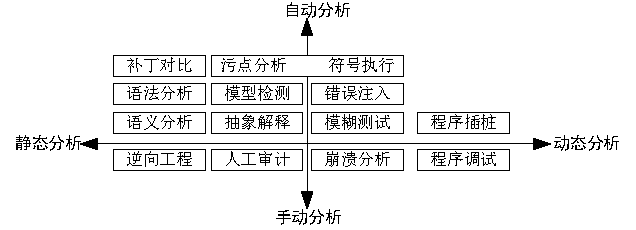
\includegraphics[scale=0.3]{chap01/根据挖掘方式分类}
\end{center}
\caption{根据挖掘方式分类}
\label{根据挖掘方式分类}
\end{figure}


\begin{figure}[htb]
\begin{center}
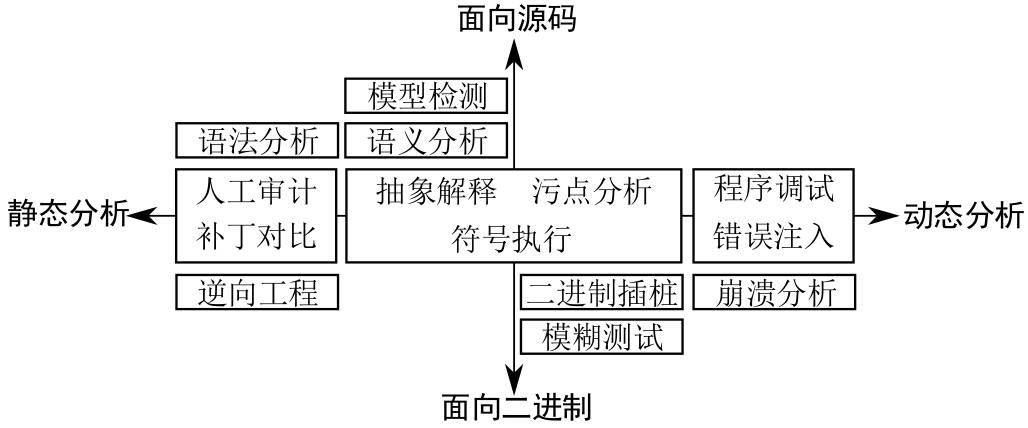
\includegraphics[scale=0.3]{chap01/根据挖掘软件类型分类}
\end{center}
\caption{根据挖掘软件类型分类}
\label{根据挖掘软件类型分类}
\end{figure}
%wb
\subsection{源代码软件静态挖掘技术}

静态挖掘技术是在不运行程序的情况下,自动的发现和报告潜在安全漏洞的技术的统称。静态分析能够全局的分析程序,不需要遍历每一个程序执行状态,从而扩大程序分析的规模。总体上,静态分析具有以下优点。(1)能够在软件生命周期的早期发现漏洞。静态分析可以在函数单元上进行单元测试,这使得错误可以在集成到大的代码模块之前被发现。进行单元测试之后,可以将精力集中在函数/单元之间的交互漏洞检测上,实现对源代码的分层检测。(2)能够检测大规模的软件。相对于人工审计,静态分析虽然压制了其报告解析能力,但是提高了检测特定漏洞的能力。相对于动态测试,不需要动态的遍历程序的每一个状态或者仅仅在源程序、中间表示上进行分析,能大大减少分析所需要的时间。同时静态分析也有以下不足。(1)在没有源代码的情况下,例如第三方库、操作系统等,静态分析需要猜测这些缺失的程序行为。(2)不能处理未域定义的程序错误行为。(3)不能检测运行时的漏洞、设计漏洞,系统管理以及由于用户的原因产生的漏洞。

%\begin{enumerate}[(1)]
%\item 能够在软件生命周期的早期发现漏洞。静态分析可以在函数单元上进行单元测试,这使得错误可以在集成到大的代码模块之前被发现。进行单元测试之后,可以将精力集中在函数/单元之间的交互漏洞检测上,实现对源代码的分层检测。
%\item 能够检测大规模的软件。相对于人工审计,静态分析虽然压制了其报告解析能力,但是提高了检测特定漏洞的能力。相对于动态测试,不需要动态的遍历程序的每一个状态或者仅仅在源程序、中间表示上进行分析,能大大减少分析所需要的时间。
%\end{enumerate}
%
%同时静态分析也有以下不足。
%
%\begin{enumerate}[(1)]
%\item 在没有源代码的情况下,例如第三方库、操作系统等,静态分析需要猜测这些缺失的程序行为。
%\item 不能处理未域定义的程序错误行为。
%\item 不能检测运行时的漏洞、设计漏洞,系统管理以及由于用户的原因产生的漏洞。
%\end{enumerate}

%大师兄
程序静态分析技术经过几十年的发展,形成了丰富的理论方法和技术手段,以程序静态分析为基础的静态漏洞挖掘方法的研究也极为深入。在词/语法分析、定理证明、抽象解释、符号执行、模型检验和机器学习等理论的支持下,静态漏洞挖掘取得了显著进展。
%大师兄

\subsubsection{词/语法分析技术}

词法分析通过对以往漏洞的分析,例如,人们发现缓冲区溢出常与某些语句或者语句组合有关(例如 strcpy, strcat),于是开发了一些通过词法分析发现缓冲区溢出漏洞的检测工具,例如 RATS\upcite{wnoauthor_cern_nodate}、 ITS4\upcite{noauthor_its4_nodate} 和Flawfinder\upcite{flawfinder_nodate} 等。此类工具对程序的语句进行遍历,并与预先建立的漏洞模式进行匹配,最后根据匹配结果报告可能的缓冲区溢出漏洞。由于这种方法不理解程序语义,所以容易产生漏报或误报。此技术一般只作为手工分析的起点。

\subsubsection{定理证明方法}

定理证明的基本思想是将源程序的语义和安全规范转换为逻辑公式,再将这些逻辑公式输入到一个定理证明器进行验证,从而将软件错误的发现过程转换为逻辑公式的证明过程。这种方法的优点是严格,能够保证通过验证的程序不存在漏洞,但它通常要求用户( 用形式逻辑语法) 提供循环不变式、过程调用的前置条件和后置条件等信息,以帮助定理证明器完成推导,因而难以实现自动化。Compaq 公司的 ESC\upcite{leino_esc/java_2000}、以色列 Tel-Aviv 大学的 CSSV\upcite{dor_cssv:_2003} 都采用定理证明方法检测程序中的缓冲区溢出漏洞。

\subsubsection{抽象解释技术}

抽象解释把程序的执行过程看成抽象状态的迁移过程,并通过抽象状态的分析确定程序的性质。为了保证分析结果的正确性,抽象解释要求初始抽象状态是初始实际状态的安全近似,且每次状态迁移都能保持正确关系。正确的抽象解释能够发现程序中的漏洞,但存在较多的误报,所以在实际使用时常常要求用户根据被测试程序的特性,选择合适的抽象域、加宽操作和解释函数等,以降低误报率。例如, Patrick Cousot 领导的项目 ASTREE\upcite{cousot_astree_2007} 采用基于抽象解释理论的程序静态分析器。ASTREE 可以检测数组越界访问、除零异常、浮点运算溢出和整数运算溢出等问题。ASTREE曾用于检验法国空中客车公司的空中巴士A340和A380系列飞机飞行控制软件,受到工业界的认可。除了ASTREE,FLUCTUAT\upcite{delmas_towards_2009} 、Coverity\upcite{almossawi_analysis_2006} 等都是采用抽象解释理论进行静态
漏洞检测的典型工具。抽象表达提供了对变量边界值的估计,但无法有效追踪变量之间的约束关系,在路径可行性判定上依然存在不足。

%\subsubsection{约束分析}
%
%约束分析是一种通过建立和求解程序的约束条件,发现程序性质的方法。基于约束分析的静态方法常将检测过程分为约束产生和约束检查两个独立步骤,前者利一组约束产生规则建立程序的约束条件,后者对建立的约束条件进行求解,进而检验程序的性质。约束分析可以处理无穷系统,而且自动化程度较高。美国加州大学Berkeley分院的 Wagner设计了一个基于约束分析的缓冲区溢出漏洞检测器BOON\upcite{noauthor_boon_nodate}。

\subsubsection{静态符号执行技术}

静态符号执行是King等人1976年在文献\upcite{king_symbolic_1976}一文中首先提出。符号执行的基本思想是,用抽象的符号表示程序中变量的值,根据程序的语义,遍历代码执行空间,来模拟程序的执行。符号执行的主要优势在于能够发现变量之间运算关系,便于理解程序的内在逻辑;在漏洞挖掘时,有利于在复杂的数据依赖关系中发现数据之间本质的约束关系,而且符号执行精确记录了路径的约束条件,可以进一步用于判断路径可行性和路径约束的完备性。

符号执行技术通过将程序的输入由具体值替换为符号变元,将程序中每条指令本身的具体计算语义映射为相应的符号计算语义,在程序控制流指导下,关注路径的分支谓词,为路径状态树中的每个叶子节点对应的程序路径推导出相应的能够到达该位置的敏感输入满足的最弱前条件。符号执行的核心,在于以等价类的形式对程序的执行路径进行标注,进而高效率地实现路径覆盖。

符号执行可以分析代码的所有语义信息,也可以只分析部分语义信息。符号执行分为过程内分析和过程间分析(又称全局分析)。过程内分析是指只对单个函数的代码进行分析,全局分析指对整个软件代码进行上下文敏感的分析。所谓上下文敏感分析是指在当前函数入口点要考虑当前的函数问调用信息和环境信息等。程序的全局分析是在过程内分析的基础上进行的,但过程内分析中包含了函数调用时就也引入了过程问分析,因此两者之间是相对独立又相互依赖的关系。

符号执行常常在对路径敏感的程序分析中使用。符号执行可以看作是程序测试与程序验证的折中方法,其优点在于它可以精确地静态模拟程序的执行。由于它跟踪了变量的所有可能取值,因此能够发现程序中细微的逻辑错误。但是在处理大程序时,程序执行的可能的路径数目随着程序尺寸的增大而呈指数级增长。在这种情况下需要对路径进行选择,选取定数量的路径进行分析。

早期静态符号执行典型系统包括Prefix\upcite{bush_static_2000}和ESP\upcite{das_esp:_2002}。W.Bush等人在1998年提出了Prefix,并在美国申请了若干专利。微软公司于1999年收购了Prefix,在Prefix基础上实现了Prefast。Prefix/Prefast已经成为微软内部标准源代码静态检验工具之一。ESP借鉴了MC由用户制定检查规则的思想,基于符号执行技术识别和保留路径上安全属性状态相关的约束条件,能够有效排除很多不可行路径。

\subsubsection{模型检测技术}

模型检验是一种针对有限状态并发系统的自动分析与验证技术,其基本思想是状态搜索。对状态空间的穷尽搜索有赖于对系统建立的有穷状态模型,以保证搜索过程的终止。模型检测的优点是能够做到完全自动化,在搜索终止时,如果性质没有满足,能够给出反例,这有利于用户对系统进行改进; 缺点是建模比较困难,且面临状态空间爆炸的问题。一般情况下,模型检查只适合用于对临时属性(如内存是否被释放、指针是否为空等)的检测。

模型检验技术最早应用于时序电路和通信协议设计的自动化检验,其基本思想是用状态迁移系统描述程序的行为,用时序逻辑、计算树逻辑或π演算公式表示系统的性质,从而将系统属性的检验问题转换为搜索不满足逻辑公式的状态系统的问题。模型检验需要遍历系统的整个状态空间,所以只能分析有限状态系统。例如,Berkeley大学的MOPS\upcite{chen_mops:_2002}、微软研究所的SLAM以及Bell实验室的UNO\upcite{holzmann_static_2002}都是基于模型检验的检测工具,它们能够发现程序中的一些字符串库函数的滥用。MOPS系统能够做到检测结果无漏报(完备性),但是MOPS是数据流不敏感的分析,无法跟踪数据依赖关系,导致MOPS误报率很高。SLAM\upcite{noauthor_slam_nodate}是一种基于谓词抽象技术的软件模型检验器,主要用于检测Windows操作系统驱动程序是否满足用户定义的属性约束。SLAM的核心技术是谓词抽象,将每个变量都抽象为只有0/1两种取值。这种过近似(Over Approximations)抽象方法导致SLAM误报较为严重。由于模型检验技术面临着状态空间爆炸的问题,在大型复杂软件的漏洞挖掘工作中仍处于探索阶段。

有些模型检验工具,例如Spin\upcite{noauthor_spin_nodate}与CBMC\upcite{noauthor_cbmc_nodate},能够直接应用于源代码,准确地捕捉程序的真实行为,精确度比较高。但是,它们要么可扩展性不好,不能应用于大规模的程序(如Spin);要么只能检查大型程序的部分状态,用作一种查错工具,不能覆盖所有的状态,不能保证找到所有的错误。另外一些模型检验工具基于谓词抽象的思想自动化抽取系统的有穷状态模型,如BLAST\upcite{beyer_software_2007}和SATABS等,它们的基本思路都是谓词抽象与CEGAR(Counter Example Guided Abstract Refinement,反例制导抽象精化)\upcite{andraus_cegar-based_2007},这也是目前主流的软件模型检验实现思路,但谓词发现以及模型精化仍是此类技术中的难点问题。


\subsubsection{基于机器学习的软件漏洞静态挖掘技术}
%随着机器学习算法的成熟,机器学习的很多方法也应用到了漏洞挖掘和软件测试之上。例如智能优化算法在模糊测试技术上的应用,AFL-go\upcite{bohme_directed_2017}利用模拟退火算法随着时间的推移分配种子变异的能量;AFL\upcite{noauthor_american_nodate}利用遗传算法框架变异种子以扩大测试的代码覆盖率;另外还有将遗传算法应用到回归测试\upcite{doungsa-ard_automatic_2007}、基于模型的模糊测试技术\upcite{sharma_applying_2014,sabharwal_prioritization_2010,you_genetic_2012,patton_genetic_2003}以及web测试\upcite{peng_new_2011}当中。

随着机器学习算法的成熟,一些研究者将机器学习的有监督、无监督算法以及神经网络算法和程序分析相结合用于挖掘软件漏洞。Padmanabhuni\upcite{padmanabhuni_predicting_2014,padmanabhuni_auditing_2016}利用有监督机器学习算法建立分类器用以检测缓冲区溢出漏洞。Neuhaus\upcite{neuhaus_predicting_2007}根据Mozilla的漏洞历史,从中提取向量,并利用机器学习算法预测哪些组件有可能出现漏洞。Zimmermann\upcite{zimmermann_searching_2010}以代码复杂度、代码混淆度等为特征预测Windows Vista中可能出现漏洞的组件。Perl\upcite{perl_vccfinder:_2015}利用github提交代码的语言类型、贡献者的fork数量等特征预测哪些提交可能出现漏洞。Grieco\upcite{grieco_toward_2016}以C语言程序中的函数调用轨迹为特征预测大规模程序中的漏洞。Yamaguchi\upcite{yamaguchi_chucky:_2013,yamaguchi_automatic_2015}利用异常检测检测源代码中缺少边界检测的情况以及使用聚类算法检测Taint-Style类型的漏洞。Rajpal\upcite{rajpal_not_2017}提出了一种基于时间递归神经网络的提高模糊测试代码覆盖率的方法。


\subsection{源代码软件动态挖掘技术}

动态测试是对程序运行时特性的测试分析,有别于静态分析检查源程序的手段,动态分析通过检查运行时的程序来获取程序特性。静态分析的结果通常对于每次程序的执行都成立,而动态分析的结果可能只对某一次或某几次运行成立。动态分析正在被广泛应用于包括系统安全分析在内的多个领域,软件工程国际会议(International Conference on Software Engineering/ICSE) 专门设立了动态分析研讨会( Workshop on Dynamic Analysis/WODA),会议的主题包括动态分析的各种研究和应用。

\subsubsection{运行时监测技术}

运行时监测(Runtime monitoring)是根据插桩的安全规范代码和检测代码在程序运行时检测是否违反安全规范。如斯坦福的Michael Martin等人的PQL(program query language)\upcite{martin_finding_2005},首先使用上下文敏感、流不敏感、基于包含的指针别名分析,找出所有可能的匹配点,然后对这些匹配点进行插桩后在运行时监测。另外像VS.Net 中使用的放在调用栈中的canary,canary值存放在用户数据和返回地址之间,一旦发现canary值被改变,则表明发生了缓冲区溢出。运行时监测首先要利用各种静态分析技术(如指针分析、别名分析、类型推断等),结合给出的安全规范,找出程序中所有可能违反安全规范的地方;然后利用代码插桩技术(包括静态插桩和动态插桩)对可能出现安全漏洞的地方插桩检测代码,同时插桩安全规范;最后利用动态检测算法在运行时检测程序是否违反安全规范。

\subsubsection{动态符号执行技术}

%\textbf{参考directed Greybox Fuzzing的introduction中关于符号执行的介绍}

基于动态符号执行的漏洞挖掘,一般将关注的程序漏洞以符号断言的形式进行描述。对每条路径的符号分析过程中,在敏感的程序点处对漏洞断言的可满足性进行判定。如确定断言为可满足,即断定当前分析路径中存在该类型漏洞。近年来,该型技术得到了较为广泛的应用。

2005年,Godefroid等学者提出的DART\upcite{godefroid_dart:_2005}系统是最早的动态测试用例生成系统。DART首先生成一个随机值作为外部变量的初始化输入,且对每个外部函数都返回一个随机值,由于随机值不能确保对程序中的每条分支都能覆盖到,因此随机测试的覆盖率通常很低。然而,DART对输入的随机值进行符号化处理,即在随机化之后,这些变量被标记为符号变量。在遇到新分支时,一条路径约束通过不断收集执行过程中的约束来生成,而下一条路径则是通过对另一分支的约束取反来生成。如果一条路径不可求解,这个约束将用具体值代入,进行化简。DART的缺点时不能处理指针语义,无法分析C语言中常见的指针操作。

CUTE\upcite{sen_cute_2006}被定义为一个混合符号执行工具,即联合了符号执行与具体执行。与DART系统类似,CUTE允许用户通过指定代码来决定哪些输入可以被符号化,这使得任意外部用户输入都可以被替代。CUTE的路径遍历是通过插桩来实现的。与DRAT相比,CUTE最大的改进是能够处理指针操作和数据结构。

斯坦福大学的Engle等学者提出的EXE\upcite{cadar_exe:_2008}系统,用于组件测试,在动态收集路径可达约束信息方面和约束路径精确求解方面的贡献较为突出。EXE系统是一个源到源的编译器。该编译器将目标应用源码中的每一个赋值和运算前都插入对EXE系统符号化执行组件的函数调用,并在程序的分支语句前插入一段调用求解器代码,对当前分支条件进行求解并产生测试用例。这样,当被EXE编译后的程序真正执行时,真实的程序执行和符号化执行交替进行,并且符号化执行从程序的具体执行中获取所需运行时信息,以收集路径可达约束。此外,EXE系统实现了一个SMT求解器 STP,该求解器包含了BV理论、ARRAY理论和整数理论。由于路径可达约束的收集和约束求解都较为精确,EXE系统生成的测试用例软件缺陷的发掘效率较高。

KLEE\upcite{cadar_klee:_2008}系统是基于EXE系统的升级,该系统将EXE系统的源到源编译器变为LLVM编译器\upcite{noauthor_llvm_nodate}。KLEE系统纯符号化执行LLVM编译出的低级指令。这些改进使得KLEE系统可以更为普适地应用于各类LLVM支持的语言程序。KLEE同样需要完整源码支持。并且由于KLEE系统采用完全符号化解释执行每一条LLVM指令,测试性能低。

SAGE\upcite{godefroid_sage:_2012}系统是微软研究院研发的动态测试用例生成系统。与之前的系统不同,SAGE系统直接对二进制程序进行动态追踪并生成测试用例。该系统采用动态二进制指令追踪工具Nirvana,监控程序执行,追踪指令执行获得程序的执行流日志。然后再离线地对日志文件进行符号化分析执行,构建路径可达约束,以便为输入可控分支生成测试用例。与EXE系统不同,SAGE系统为了能够对大规模程序进行分析,采取了一系列的简化措施:(1)SAGE系统为了简化约束收集和求解的复杂性,忽略对非线性约束的收集与求解。(2)SAGE 系统不对程序中的指针进行分析。相对于EXE系统,以上简化措施一定程度上加快了SAGE系统对大型目标软件的测试用例生成速度,然而这却以损失测试用例对路径覆盖指导的精度为代价。SAGE系统生成的测试用例中有接近60\%的测试用例无法准确指导程序覆盖目标路径。此外,SAGE系统对日志中的所有指令流都采用完全符号化解释执行,导致符号化执行时间占全系统工作时间的25\%。这就抵消了部分由前面所述简化操作带来的性能提升。

伯克利大学的SmartFuzz\upcite{molnar_dynamic_2009}系统与SAGE系统类似,采用了基于Linux下的二进制指令追踪工具Valgrind追踪程序执行和在线约束收集方式。SmartFuzz系统仅支持整数溢出缺陷的发掘。

李根设计和实现了Hunter\upcite{hunter__2010}系统,提出了基于路径完备可达理论以及污点可控指针分析的算法,能有效覆盖基于攻击面污点输入可达的测试路径,由于采用了基于虚拟机平台的符号化执行及线程监控技术,具有良好的跨平台兼容性。

在符号执行的实际应用中,还面临这许多问题,比如符号执行的精度
问题\upcite{godefroid_higher-order_2011},复杂的输入格式问题\upcite{majumdar_directed_2007,godefroid_grammar-based_2008},路径爆炸问题\upcite{boonstoppel_rwset:_2008,godefroid_compositional_2010},符号指针问题\upcite{trtik_symbolic_2014}等。其中路径爆炸问题是一个符号执行研究的一个重要分支。其主要形成原因在于,每一个分支条件语句都可能导致当前路径再分支出一条新的路径进行分析计算,而这是以指数的形式增长的。尤其体现在程序中存在跳转谓词与输入变元相关的循环结构时。

当前的解决办法包括:为循环引入“执行计数变量”,通过进行“执行计数变量”与输入的关联和程序中的变量与“执行计数变量”的关联,实现将程序中“循环次数相关”的变量的值完全通过输入相关属性表达的抽象计算。作为一种
摘要计算技术,约减了循环处理中的分析计算量;在对大量实际应用程序分析的基础上,仅仅为输入的“长度”和“部分输入前缀字符”引入符号变元,进行符号计算。该方法理论上并不是完备的,但实际应用中能覆盖较多的缓冲区溢出情形;有些相关研究提出综合使用程序切片、抽象解释、循环不变量计算和循环单值识别等技术对循环执行次数的上界进行估算:利用程序切片获取与循环结束判断条件相关的变量和语句,进而在此基础上进行抽象解释,对相关变量的取值范围近似获取。在经过循环不变量分析和循环单值识别后,进一步剔出变量值域,最终获取循环次数的估计值。

Godefroid等在文献中通过为包含归约变量的输入相关的循环计算循环摘要\upcite{godefroid_automatic_2011},避免了对每条循环相关分支的分析。但仅仅适用于循环中变量与归约变量存在线性关系的情况下;瑞士的开源项目S2E\upcite{chipounov_s2e:_2011}提出了选择式符号执行的思路:仅仅对关注的程序部分(某一特定代码模块或访问某一特定数据的代码部分)进行符号执行,在关注的程序部分和不关注的程序部分之间,维护确保分析状态一致性的转换机制。

%\subsubsection{导向符号执行技术}

导向符号执行是符号执行中利用程序分析以及约束求解技术有效的搜索可能目标路径空间的一个方向\upcite{ma_directed_2011}。Haller\upcite{haller_dowsing_2013}提出了一种导向危险库函数以及危险操作的区域的符号执行方法。另外一些研究者将导向符号执行应用到程序补丁验证\upcite{bohme_partition-based_2013,marinescu_katch:_2013,miller_empirical_1990}、增加符号执行代码覆盖率\upcite{xu_directed_2010}、减少静态分析误报\upcite{christakis_guiding_2016}以及崩溃重现之上\upcite{jin_bugredux:_2012, ros_sler_reconstructing_2013}。但是导向符号执行是重量级的,需要大量的程序分析以及约束求解。

%\subsubsection{约束求解技术技术}
%
%使用动态符号执行进行测试数据生成的基础在于底层的约束求解技术一一预期的程序路径约束最终需要表达为约束求解器所识别的语言,并由其判断可满足性以及给出对应的数据样本。
%
%lp\_solve\upcite{buttrey_calling_2005}是一个开源的线性规划求解器,其可以求解纯线性、整型、半连续及Special Ordered Sets\upcite{beale_global_1976}模型。我们将路径约束的求解问题转化为了在路径约束变量上的线性规划问题。虽然lp\_solve的求解能力不足以覆盖一般程序中出现的所有运算操作,如乘法、除法、位运算,但是已经足够覆盖足够的范围,即并行化现有方法。
%
%另一方面,如果需要表达能力更强的约束求解器,则可以选择SMT(Satisfiability Modulo Theories)\upcite{ranise_satisfiability_2006}求解器。SMT问题是布尔可满足性问题的扩展,前者将后者公式中的布尔变量替换为了由不同底层理论(如整型、实数、位向量甚至是不同的复杂数据结构)所支撑的谓词。因而,相比其他可用于约束求解的技术而言,SMT求解器有着更加强大的表达能力。当前的SMT求解器可直接支持包含如数组、结构体、枚举量之类的真实程序中经常出现的数据结构的模型,而避免了由包含这些结构的程序路径约束向表达能力较弱的求解器语言转换时可能导致的语义丢失。
%
%STP(Simple Theory Prover,简单理论证明器)\upcite{noauthor_simple_nodate}是用于求解定长比特向量和一维数组的逻辑公式可满足性的决策程序。简单的说STP就是一种用于求解特定逻辑方程组的工具。STP有其自身的语言规范,包括提供的接口函数和语法规则。接口函数包括比特向量的拼接和抽取、移位、符号扩展、有符号和无符号的算术操作(加减乘除取模等)和逻辑位操作等。还提供了比特向量间的有/无符号比较谓词(大于等于小于)。
%
%只要符号执行提取的路径条件符合 STP 的语法规范,就可以利用 STP 进行求解,从而判断一条具体的路径是否成立,如成立,则可得到对应该路径的测试用例。

\subsubsection{模糊测试技术}

Miller等\upcite{miller_empirical_1990}在1991年首次提出了模糊测试的概念,目的是检测UNIX命令行工具程序的可靠性。因为事先不知道程序、输入的结构信息,最先的模糊测试被称为黑盒模糊测试。模糊测试通过不同的方式(例如比特反转、边界值替换、输入块删除和复制)变异程序输入,从而产生大量的畸形输入;然后将畸形输入反馈给程序执行,观察程序是否异常。这个简单且有效的方法奠定了模糊测试的基础。下面从三个方面概述模糊测试技术。

(1)基于模型的黑盒模糊测试技术

传统的黑盒测试\upcite{noauthor_zzuf_nodate}没有考虑输入的结构信息,以至于变异的绝大部分输入因为不符合正确的格式标准而只能检测程序的一小部分路径。这种情况导致了传统的黑盒模糊测试不能挖掘程序的深层次信息。为了解决这个问题,研究者提出了基于模型的黑盒模糊测试框架例如Peach\upcite{noauthor_peach_nodate}和Spike\upcite{noauthor_immunity_nodate}。本质上,当输入是有格式的文件数据或者协议数据时,测试用例变异需要保证程序输入能够满足格式规范,从而通过程序的格式检测。这种方法增加了生成的测试输入的有效性,从而能够测试更深更关键的程序状态。但是,有的文件或报文格式并未公开,如何获得准确的输入格式或者绕过对输入格
式的校验成为研究的重点问题\upcite{li_automatic_2011,kim_efficient_2011,gorbunov_autofuzz:_2010,lin_automatic_2010,wang_taintscope:_2010}。另外还有一些研究者将遗传算法应用到基于模型的黑盒测试技术当中\upcite{sharma_applying_2014,sabharwal_prioritization_2010,you_genetic_2012,patton_genetic_2003}。

%随着机器学习算法的成熟,机器学习的很多方法也应用到了漏洞挖掘和软件测试之上。例如智能优化算法在模糊测试技术上的应用,AFL-go\upcite{bohme_directed_2017}利用模拟退火算法随着时间的推移分配种子变异的能量;AFL\upcite{noauthor_american_nodate}利用遗传算法框架变异种子以扩大测试的代码覆盖率;另外还有将遗传算法应用到回归测试\upcite{doungsa-ard_automatic_2007}、基于模型的模糊测试技术\upcite{sharma_applying_2014,sabharwal_prioritization_2010,you_genetic_2012,patton_genetic_2003}以及web测试\upcite{peng_new_2011}当中。

(2)覆盖率导向的模糊测试技术

覆盖率导向的模糊测试是通过一系列方法增加种子语料库代码覆盖率的技术。其出发点是基于这样一个判断“如果要检测某个程序元素$e$中的漏洞,种子语料库中就必须要包含一个种子在程序执行时能够到达$e$”,这里$e$可以是一个语句、一个基本块或者其他的区域。在执行一个测试用例时,覆盖率导向的模糊测试工具\upcite{bohme_coverage-based_2016,noauthor_american_nodate,rawat_vuzzer:_2017,sparks_automated_2007,noauthor_libfuzzer_nodate}使用轻量级的代码插桩在运行时收集代码覆盖信息。AFLFast\upcite{bohme_coverage-based_2016}设计了一种路径概率计算方式,变异概率较低的路径对应的测试用例能触发更多的路径,从而增加代码覆盖率。同时,设计一种测试用例变异能量分配方式,驱动模糊测试多变异遍历概率低的路径。Vuzzer\upcite{rawat_vuzzer:_2017}为每一个基本块设置了一个权重,并且计算每条路径的权重,在模糊测试时着重测试更可能触发漏洞的路径。Sparks\upcite{sparks_automated_2007}使用了遗传算法的思想变异定长的种子语料库并根据输入数据格式以遍历更深的路径。

(3)目标区域导向的模糊测试技术

目标区域导向的模糊测试是指在指定目标区域的情况下,通过设定一系列标准,驱动模糊测试执行到目标区域的技术。Marcel Böhme在AFL的基础上开发了AFL-go工具\upcite{bohme_directed_2017}。该工具定义了每个测试用例和目标区域的距离,并设计一种基于模拟退火的能量分配策略,使得随着时间的增加到目标区域距离较小的测试用例变异次数增加,而到目标区域距离较大的测试用例变异次数减少,以此增加测试用例经过目标区域的概率。虽然AFL-go在一定程度上实现了导向性,但是其变异的方式依然是无序的。基于此分析,论文第五章提出了一种细粒度变异的导向模糊测试方法,根据关键字段权重变异测试用例以达到快速导向并发现更多漏洞的目的。

还有另外的研究者提出了基于污点分析的导向模糊测试技术\upcite{henderson_decaf:_2017, newsome_dynamic_2005}。该技术利用污点分析方法判断哪些字段对导向目标区域具有关键作用,变异这些字段产生的测试用例能够以更大的可能性遍历到目标区域。通过这种方式能够极大的减少需要遍历的程序状态空间。

%\upcite{meng_assisting_2017}

\section{源代码软件漏洞挖掘的关键问题}

%静态分析和动态分析是源代码软件漏洞挖掘的两个主要方向。
通过对比分析现有的源代码软件漏洞挖掘方法及工具,可发现源代码软件漏洞挖掘存在以下发展趋势\upcite{zhangliyong_2011}。%抄源代码安全性分析
\begin{enumerate}[(1)]
\item 从内置安全规则到可扩展安全规则。现在的源代码安全分析工具都会提供多种配置机制和接口,供分析人员根据实际需要编写程序实现自定义的安全分析\upcite{noauthor_code_nodate,ashcraft_using_2002}。
\item 从依靠抽象语法树的词法匹配的方式到到多中间表示混合匹配的方式。抽象语法树只能识别出程序中的敏感操作,且会产生大量的误报,将其他的中间表示形式,如控制流图和数据流图综合考虑能大大减少误报。
%\item 从单类型源代码漏洞分析到多类型漏洞分析。
\item 从单纯的程序员指导程序分析到以程序员为辅助的自动程序分析。程序员在安全分析中的参与比重越来越小。现在许多模型检测、抽象解释工具的使用,只需要程序员在可能发生漏洞的区域添加注释就可以完成。而另外一些分析工具\upcite{gregor_stllint:_2006,noauthor_splint_nodate},因为使用了更为复杂的语义提取方式,程序员的参与度进一步减少。
\item 使用形式化方法辅助软件测试。软件测试方法本质上是遍历程序状态空间,容易引起状态空间爆炸。形式化方法通过提供语义等价的程序转换,能够减少状态空间。将二者结合,能够发现软件测试检测不了的漏洞。
\item 使用源代码的直接或者间接信息辅助软件测试。越来越多的从源代码中获取的信息用于帮助符号执行、模糊测试等软件测试方法,例如程序的执行路径\upcite{marinescu_katch:_2013}、以及程序基本块的距离\upcite{bohme_directed_2017}。
\end{enumerate}

通过多年的研究,源代码软件漏洞挖掘在上述各方面取得了不少进展,但仍然有很多问题有待解决。

%漏洞挖掘的最终目的是产生能够触发软件漏洞的测试用例。一般而言,测试用例的产生需要动态遍历程序状态空间。但是随着软件规模的增加,程序状态空间会产生爆炸性的增长,使得遍历所有的程序空间变得不可行。现在主流的挖掘流程是首先利用静态程序分析标定可能出现漏洞的代码区域——可疑区域,然后动态测试这些代码区域,从而减少测试的程序状态空间。所以,
%可疑区域的标定和动态测试是源代码软件漏洞挖掘的两个重要研究内容。虽然国内外研究者在这两个方面提出了很多的方法,例如危险函数搜索、模式匹配用于标定目标区域,模糊测试、符号执行用于动态测试,但在实际漏洞挖掘的过程中,仍有许多问题待解决。
%大体上源代码软件漏洞挖掘的关键问题可以分为两大类:可疑区域的标定问题和动态测试问题。虽然国内外学者对可疑区域标定以及动态测试已经进行了多年的研究,但仍然存在很多问题有待解决。
%可疑区域的标定一般是根据某类漏洞的特征设计固定的漏洞模式,然后利用字符串匹配方法或者在中间表示上遍历进行,此方式误报率高且标定的漏洞种类单一。此外,对于缓冲区溢出这种成因比较复杂的漏洞,即使使用了多种
%主流的动态测试方法包括符号执行和模糊测试。符号执行本质上需要遍历所有的程序状态空间,具有典型的路径爆炸问题;模糊测试利用随机输入遍历程序状态空间,相对于符号执行代码覆盖率较低,不能有效覆盖可疑区域。
%符号执行具有典型的路径爆炸问题而模糊测试具有路径覆盖率低且无法导向问题。
%综上,源代码软件漏洞挖掘的关键问题可以分为三类:多种类漏洞可疑区域标定问题、符号执行路径爆炸问题以及模糊测试导向问题。

%因此如何利用静态分析方法粗定位漏洞区域、
%相对于二进制软件,源代码软件包含更多的信息,主要表现在源代码具有更多更精确的中间表示形式。利用
%所以高精度的静态分析和可控的动态挖掘技术是源代码软件漏洞挖掘的重要研究方向。从另一方面来讲,

%syf
%源代码软件漏洞挖掘技术经过多年的研究和发展,逐渐积累了丰富了理论知识,产
%生了很多可用于漏洞挖掘的技术手段,但从软件漏洞挖掘本身的特性和当前软件
%漏洞挖掘采用的技术手段的特性上看,仍然面对以下主要问题:
%syf

(1)多种类源代码软件漏洞精确静态挖掘问题

%单一的中间表示表达能力有限的问题
%wb
%静态挖掘出潜在的软件漏洞是漏洞挖掘的出发点。论文认为挖掘包括检测和
%挖掘两个层次。论文将只有在漏洞真实触发时才能准确判定漏洞的方法称为漏洞
%检测;将不需要真实触发漏洞就能准确判定漏洞的方法称为漏洞挖掘。
%wb
繁多的源代码漏洞种类给漏洞挖掘带来了困难。由于不同种类的漏洞具有不同的特 %copy from syf
征,现存的基于模式匹配的漏洞挖掘工具,一方面不能检测多种源代码软件漏洞,另外一方面则会造成很高的误报。例如对于基于抽象语法树匹配的缓冲区溢出漏洞检测,通过遍历所有程序语句的抽象语法树虽然可以找到所有的内存拷贝函数,但是无法探知程序中是否对内存拷贝操作进行了边界检测;另外,抽象语法树对于缓冲区循环写造成的缓冲区溢出漏洞则完全没有检测能力。而上述问题可以通过将抽象语法树、控制流图、数据流图结合来解决。所以,研究多种中间表示的聚合方式并在此之上研究各类源代码漏洞的挖掘方法是一个关键问题。

(2)机器学习算法和源代码软件漏洞挖掘的结合问题

一般的漏洞静态挖掘方法则局限于特定的漏洞模式,若模式限制条件过强,则漏报率较高;若限制条件过弱,则误报率较高。对于缓冲区溢出漏洞,影响漏洞的静态特征有很多种,漏洞的形成是多个特征综合作用的结果。在源代码中这些静态特征可以通过各种中间表示获取,若将漏洞挖掘转换成机器学习中的分类问题,则能从以往的漏洞数据中学习出规律,解决上述问题。因此如何将机器学习算法和漏洞挖掘结合也是一个关键问题。

%将机器学习算法结合到漏洞挖掘上,则能不局限于特定的漏洞模式,根据以往的漏洞和非漏洞程序学习出一个综合的分类模型。例如,对于缓冲区溢出漏洞,影响漏洞的特征有很多种,漏洞的形成是多个特征综合作用的结果。而一般的漏洞静态挖掘方法则局限于特定的漏洞模式,若模式限制条件过强,则漏报率较高;若限制条件过弱,则误报率较高。
%若将漏洞挖掘转换成机器学习中的分类问题,则能从以往的漏洞数据中学习出规律,解决上述问题。
%因此如何将机器学习算法和漏洞挖掘结合也是一个关键问题。
%面对检测对象,如何将漏洞挖掘问题转换成机器学习中的分类问题是是漏洞挖掘和机器学习结合的关键。所以面对特殊的缓冲区溢出漏洞,如何选取特征、选取哪些特征。
%也会造成漏报率较高的问题。每年都会有大量的漏洞被曝出,如何利用已知的漏洞并从中建立模型降低可疑区域标定的漏报率也是一个关键问题。


(3)源代码静态信息辅助的模糊测试导向问题

模糊测试已被证明是一种非常强大的软件漏洞测试方法,是工业界和学术界研究的热点。但是模糊测试同样有它的局限性,盲目的随机的变异测试用例很难到达测试程序的特定路径,导致一些漏洞很难被触发。而在源代码中,漏洞可疑区域及其与其他代码的距离信息可以通过静态分析获取。如何利用这些信息指导模糊测试,动态的测试目标区域也是一个关键问题

(4)符号执行循环程序引起的路径爆炸问题

动态符号执行作为典型的动态测试方法,在理论上能够有效遍历目标软件的 %wb
状态空间,从而深度挖掘软件中存在的漏洞。但实际检测中,随着程序规模增大,符号执行必然会引起路径爆炸。导致符号执行路径空间爆炸的一个非常关键的因素是程序中的循环语句。在分析循环程序时,符号执行每一次进入循环体内部,都需要构造两条分支路径,分别对应了循环条件为真或假的情况,导致分支路径总数目随着循环次数的增加呈指数级增加。在源代码基础上的形式化方法能够将循环语义等价的转化成一个顺序语句,以缓解循环引起的路径爆炸问题。所以如何将形式化方法和符号执行结合缓解路径爆炸也是一个关键问题。
。
%所以,如何利用模糊测试动态的产生测试用例到达可疑区域也是一个关键问题。

\section{论文的研究思路与主要研究内容}
%wb
源代码漏洞挖掘是一项系统性的工作,只有融合多种理论、方法和技术才能挖
出潜在漏洞。软件漏洞挖掘不只是经验性的工作,而应该作为系统性的工程
来考虑。源代码软件漏洞挖掘起源于程序分析与测试领域,虽然有许多理论方法
支撑,但是各种方法都有其局限性。使用单一挖掘方法来发现软件漏洞越来越难,
只有系统性地看待软件漏洞挖掘问题,才能有所突破。

随着软件安全工程的引入,很多曾经挖掘出大量有价值漏洞的方法与工具在挖掘漏洞方面的优势越来越不明显。需要借鉴这些方法经验,研究新的挖掘思路。论文的研究对象是C/C++源代码软件,不涉及其他内存安全的语言,例如java、C\#等。
%wb
论文系统的研究了现有的源代码软件漏洞挖掘基础理论和方法,理清了这些理论和方法的脉络关系,明确了这些方法的优点和不足,并在此基础上提出了论文的漏洞挖掘思路和方法。论文的基本思路是:首先针对现有的基于模式匹配的挖掘方法不能精确挖掘多种类源代码软件漏洞的问题,研究将抽象语法树、控制流图和数据流图三种中间表示聚合的方法,并利用遍历聚合后的表示形式——程序性质图,挖掘各类源代码漏洞;
其次,
%针对基于程序性质图挖掘缓冲区溢出漏洞时漏报率较高的问题,
针对缓冲区溢出漏洞静态挖掘方法精确度不高的问题,利用缓冲区溢出漏洞的程序静态特征,研究基于机器学习的缓冲区溢出漏洞挖掘方法,
%用以平衡漏报率和误报率;
提高挖掘精度;随后,针对符号执行的路径爆炸问题,研究结合静态程序分析的高效符号执行算法,以控制符号执行规模;最后,考虑到现有导向模糊测试方法不能细粒度导向的问题,在利用时间递归神经网络训练测试用例的关键字段、累积关键字段权重的基础上,研究细粒度变异的导向模糊测试技术,增强导向模糊测试的效率以及漏洞挖掘的能力。

主要研究内容包括:

(1)基于程序性质图的源代码软件漏洞挖掘方法研究

基于模式匹配挖掘多种类源代码漏洞必须结合多种中间表示形式。论文研究了多种中间表示聚合的方法。该方法利用语法解析器解析源代码,依次生成语法分析树、抽象语法树、控制流图、数据流图。在将抽象语法树、控制流图以及数据流图聚合成程序性质图的基础上,定义并利用程序性质图的各种遍历方法,挖掘多种源代码漏洞。

(2)基于有机器学习的缓冲区溢出漏洞挖掘方法研究

针对缓冲区溢出漏洞挖掘精确度不高的问题,利用缓冲区溢出漏洞的程序静态特征,研究基于有机器学习的缓冲区溢出漏洞挖掘方法。该方法将22种程序静态特征约简成7类,分别是sink类型、缓冲区位置、容器、索引/地址/长度复杂度、边界检测、循环/条件/函数调用深度以及是否输入可控。通过扩展的程序性质图检测缓冲区溢出漏洞的各种静态特征并将其向量化,利用有监督机器学习算法在已标签的训练集上训练分类器。此分类器可用于在新的源代码中挖掘缓冲区溢出漏洞。

(3)基于细粒度变异的导向模糊测试技术研究

针对导向模糊测试的测试用例变异具有盲目性的问题,研究了一种细粒度变异的导向模糊测试技术。
该技术首先利用导向模糊测试收集测试用例;然后利用时间递归神经网络训练出一个模型,用于判断哪些字段对靠近目标区域其关键作用,同时收集每个字段的权重;在动态执行测试用例之前,利用上述模型判断当前测试用例中哪些属于关键字段并根据字段权重进行定向的变异。本方法能够更细粒度的变异指定字段,很大程度上消除模糊测试变异的盲目性,从而提高导向模糊测试的效率。

(4)结合静态分析的高效符号执行技术研究

导致符号执行路径空间爆炸的一个非常关键的因素是程序中的循环语句。在分析循环程序时,符号执行每一次进入循环体内部,都需要构造两条分支路径,分别对应了循环条件为真或假的情况。分支路径数目随着循环次数的增加呈指数级增加。
针对上述问题,研究了一种基于抽象解释的高效符号执行技术。给定待分析的源程序,首先解析出程序的控制流图。区别于其他符号执行技术,新技术通过静态程序分析方法,从程序的控制流图中计算出循环程序的不变式,然后通过用循环不变式代替循环,形成新的控制流图。在新的控制流图上进行符号执行,将会大幅减少符号执行的路径数量。




\section{论文的组织结构}

论文的结构排如图\ref{论文的组织结构}所示。

第一章为绪论,介绍课题的研究背景与意义,概述软件漏洞挖掘领域的国内外研究现状与进展,阐述论文的研究思路和主要研究内容。

第二章介绍源代码软件漏洞挖掘的基础知识和动态符号执行测试方法。介绍的基础知识包括:源代码的四种中间表示形式、源代码漏洞分类以及静态程序分析的理论基础。

第三章介绍基于程序性质图的源代码软件漏洞挖掘方法。介绍将抽象语法树、控制流图和数据流图三种中间表示用性质图进行聚合的方法,并利用遍历聚合后的表示形式——程序性质图,挖掘各类源代码漏洞的方法。介绍了缓冲区溢出漏洞的程序静态特征以及基于机器学习的缓冲区溢出漏洞挖掘方法。此章节属于纯静态分析,并不能产生导致程序崩溃的测试用例,旨在为动态测试标定目标区域,缩小测试范围。

第四章介绍基于细粒度变异的导向模糊测试技术。介绍如何利用时间递归神经网络获取关键字段以及如何计算关键字段权重;介绍在动态测试时,如何利用关键字段以及关键字段权重进行细粒度变异。

第五章介绍结合静态程序分析的高效符号执行技术。介绍了基于抽象解释的静态程序分析技术,设计了基于静态程序分析的高效符号执行方法。


第六章总结全文,并展望继续研究的方向。


\begin{figure}[htb]
\begin{center}
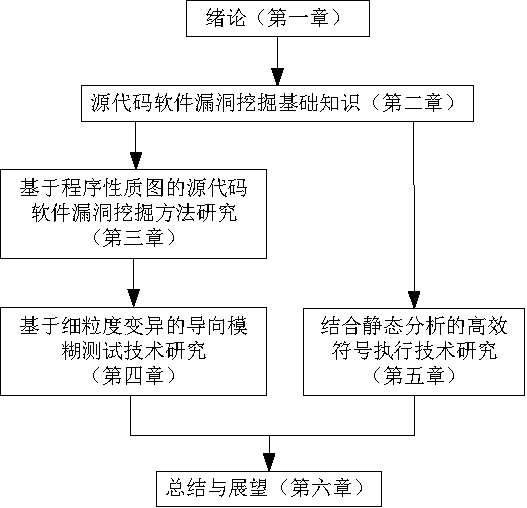
\includegraphics[scale=1.2]{chap01/论文的组织结构}
\end{center}
\caption{论文的组织结构}
\label{论文的组织结构}
\end{figure}

\chapter{源代码软件漏洞挖掘基础知识}

为了更好的介绍源代码漏洞挖掘后续章节研究工作,本章首先介绍了源代码的各种中间表示形式;其次,根据需要的中间表示数量的不同,给予源代码软件漏洞三种描述形式;然后,介绍了程序分析理论基础;最后,介绍了动态符号执行技术。

%常规软件测试方法用于分析源代码软件时尚有诸多问题需要探讨。漏洞挖掘的基本理论方法都源于程序分析与验证领域,尽管很多分析方法都得到了深入的研究,但这些方法通常单独或简单组合后被用于挖掘源代码软件中的漏洞,方法系统性的组合应用尚需要进一步摸索。因此,需要先理清不同分析方法的特点,找准其在系统性漏洞挖掘中的位置,为后续各章做铺垫。
%
%本章主要分析源代码软件测试的基础理论与方法,探讨了典型的静态程序分析、污点分析、符号执行和模糊测试等方法的基本原理及其在漏洞挖掘方面的应用。

\section{源代码中间表示形式}

因为源代码呈现出来的复杂性,在程序分析以及编译器设计技术里,研究人员提出了很多很多的中间表示用于表达程序。其中,语法分析树(Parsing Tree,PT)是语法解析器的直接产出结果。
%也是生成另外三个基本中间表示即抽象语法树(Abstract Syntax Tree,AST)、控制流图(Control Flow Graph,CFG)以及数据流图(Data Flow Graph,DFG)的基础。

\subsection{语法分析树}

语法分析树能够完全的反映程序语句的结构,以及如何将语句串联成一个完整的程序。输入一个程序,解析器根据语法文件辨别每一个终结符和非终结符,将这些标识符连接之后会得到语法分析树。语法分析树能够展示编程语言元素的类别、结构以及相互之间的关系,表现形式冗余性以及对微小改动非常敏感。图\ref{一个简单的实例程序}是一个简单的示意程序,变量x接受由外部输入函数fun得到的数据,y是x的乘法运算的结果,vul\_fun函数是一个漏洞函数。图\ref{语法分析树示例}是图\ref{一个简单的实例程序}的语法分析树示意图,其根节点是一个函数{(FUNC)},FUNC只有一个复合语句子节点{(CMPD)},复合语句包含两个语句{(STMT)}分别为赋值语句{(ASSIGN)}和跳转语句{(IF)}。


\begin{figure}[h]
\begin{lstlisting}[language=C]
void fun()
{
	int x = input();
	if(x < MAX)
	{
		int y = 2 * x;
		vul_fun(y);
	}
}
\end{lstlisting}
\caption{一个简单的实例程序}
\label{一个简单的实例程序}
\end{figure}


\begin{figure}[htp]
\centering
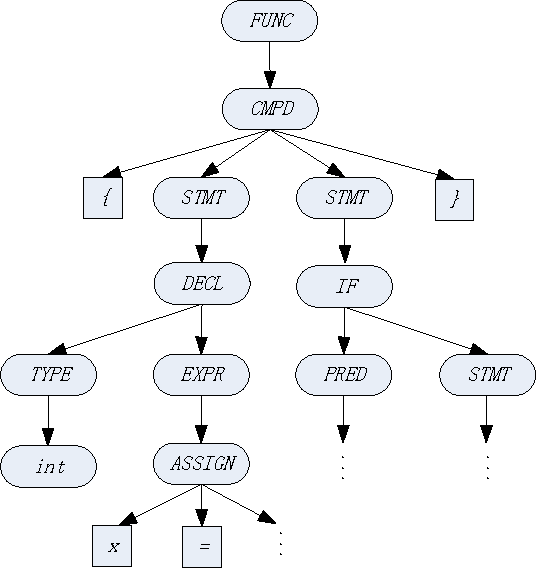
\includegraphics{语法分析树示意图}
\caption{图\ref{一个简单的实例程序}的语法分析树}
\label{语法分析树示例}
\end{figure}

\subsection{抽象语法树}

抽象语法树是语法分析树生成的最基本的中间表示,也是生成其他中间表示的基础。抽象语法树详尽的展示了操作数和操作符如何组成程序表达式以及语句,进而展示程序的整体形式。不同于语法分析树,抽象语法树不讲究和程序的每个token表示完全一致,其更偏向于语义的相似性。例如,两个用逗号隔开的变量声明将会产生两个连续的变量声明语法树。

抽象语法树是有顺序的树结构,内部节点是操作符(例如“+”和“=”)而叶子节点是操作数(例如常量和标识符)。图\ref{一个简单的实例程序}的抽象语法树如图\ref{抽象语法树示意图}所示。可以看出抽象语法树中删除了大括号和分号,另外函数调用节点{(CALL)}直接和赋值表达式相连,而语法分析树中在发现函数调用节点之前则需要遍历中间的所有节点。抽象语法树非常适合于简单的代码转换,经常被用来检验源代码的相似性\upcite{baxter_clone_1998,yamaguchi_generalized_2012}。但是抽象语法树不适用于更复杂的代码分析,例如死代码和以及未初始化的变量的检测,其原因是抽象语法树不能提供明显的控制流和数据流信息。


\begin{figure}[htp]
\centering
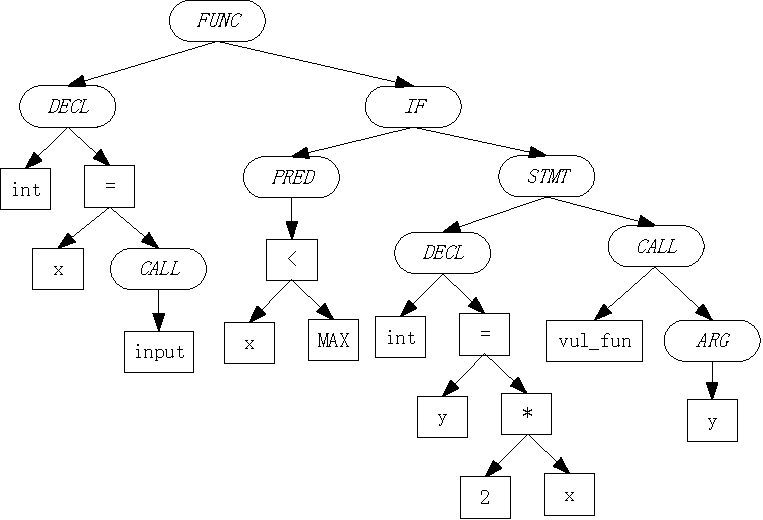
\includegraphics{chap02/抽象语法树示意图}
\caption{图\ref{一个简单的实例程序}的抽象语法树示意图}
\label{抽象语法树示意图}
\end{figure}

\subsection{控制流图}

控制流图能够描述程序语句的执行顺序以及为了执行某个语句哪些条件必须满足。无论是一般程序语句还是控制语句都用节点表示,节点之间用有向边连接以传递控制关系。相对于抽象语法树,控制流图的每条边都有一个标签$true$、$false$以及$true$分别表示控制语句的二类出边以及连接其他语句的边。图\ref{一个简单的实例程序}的控制流图如图\ref{抽象语法树示意图}所示。

控制流图在程序安全性分析中应用非常广泛,例如已知危险操作的变种\upcite{gascon_structural_2013}以及引导符号执行\upcite{sparks_automated_2007}等。另外,控制流图也已经被用在逆向工程中以帮助程序理解。虽然控制流图能够展示语句的执行顺序,但其不能提供数据流信息。在分析可疑漏洞时,不能判定某个语句是否可以被攻击者控制。

\begin{figure}[htp]
\centering
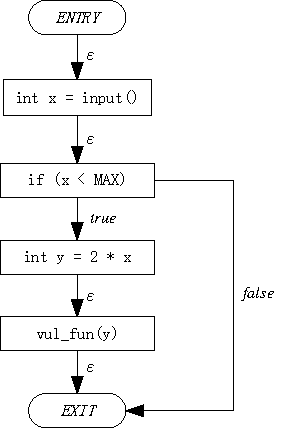
\includegraphics{控制流图}
\caption{图\ref{一个简单的实例程序}的控制流图}
\label{控制流图}
\end{figure}

\subsection{数据流图}

数据流图能够表示程序的语句之间数据依赖关系,数据流边连接的节点之间语句与语句之间的执行顺序。在数据流图上,可以不实际运行程序,直接考察数据的转移情况,从而获取数据流属性信息。图\ref{一个简单的实例程序}的数据流图如图\ref{程序数据流图}所示。变量x从声明语句传递到两个语句if(x<MAX)和int\ y = 2*x,变量y从声明语句传递到vul\_fun(y)。。

\begin{figure}[htp]
\centering
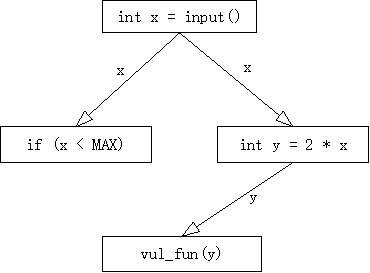
\includegraphics{chap02/程序数据流图}
\caption{图\ref{一个简单的实例程序}的程序数据流图}
\label{程序数据流图}
\end{figure}

\section{源代码漏洞描述}

源代码漏洞挖掘方法通常建立在不同的中间表示之上,根据描述源代码漏洞所需中间表示数量的不同,可以将源代码漏洞描述分为三类\upcite{yamaguchi_modeling_2014}:(1)基于抽象语法树的源代码漏洞描述;(2)基于控制流的源代码漏洞描述;(3)基于污染传播的源代码漏洞描述。不同种类不但描述的漏洞种类不同,而且对特定漏洞的描述精度也不相同。

\subsection{基于抽象语法树的源代码漏洞描述}

抽象语法树中可以获取源代码的每一个函数调用、语句甚至每一个操作数和操作符。所以利用抽象语法树可以获取攻击者可控的输入语句,敏感操作语句以及边界检测,但是不能检测出语句之间的关系。通过抽象语法树可以描述以下三类源代码漏洞:

\begin{enumerate}[(1)]
\item 不安全的参数使用。不安全的参数是引起源代码漏洞的一个重要原因。例如,格式化字符串漏洞的一个重要重要的一个特征是传递给$printf$和$sprintf$的格式化字符串受攻击者控制。所以若仅仅使用抽象语法树描述时,格式化字符串漏洞可以描述为“$printf$,$sprintf$,$fprintf$的格式化字符串不是常量”;
\item 整数溢出。当内存分配函数(alloc*)的表示内存分配大小的参数存在复杂算术运算时,整数溢出漏洞就有可能发生;
\item 数据类型错误使用。很多漏洞是由于数据类型不正确的转换引起的,例如,造成缓冲区溢出漏洞的一个重要原因就是缓冲区在初始化时,内存大小的运算未进行正确的转换和验证。在进行赋值操作时,如果右操作数的位宽比左操作数大则会发生整数截断。
\end{enumerate}

综上,下面给出基于抽象语法树的源代码漏洞描述。

\begin{definition}
\label{基于抽象语法树的源代码漏洞描述}
基于抽象语法树的源代码漏洞可以用一个二元组$(M_0,M_1)$表示,表示满足$M_0$而不满足$M_1$的所有的语句。其中,$M_0$和$M_1$表示两个谓词描述。
\end{definition}

利用抽象语法树挖掘源代码漏洞是非常有效的,但是其既不能完全表达攻击者可控的变量和敏感区域的关系。所以仅仅使用抽象语法树会产生非常多的误报。下一小节将会阐述控制流图是如何帮助部分的解决这个问题。

\subsection{基于控制流的源代码漏洞描述}

因为在控制流图中可以获取程序的执行顺序,很多源代码漏洞不但需要抽象语法树,还需要控制流图才能检测,具体漏洞类型如下所示:

\begin{enumerate}[(1)]
\item 内存泄露。很多漏洞的产生是因为分配的内存没有正确的释放。内存泄露会导致程序崩溃,另外也可以导致其他的漏洞;
\item UAF漏洞。若一个内存区域在释放后继续使用则会导致程序崩溃或者任意代码执行。此漏洞触发的主要原因是表面上无关的函数调用语句之间复杂的控制流交互关系。使用控制流分析可以轻易的得出内存释放和内存使用之间是否有控制依赖关系;
\end{enumerate}
上面两种情况,产生漏洞的原因都和控制流图上的某一条路径有关。例如,内存泄露是在一条控制流路径上内存被分配给一个变量,但在路径结束之前没有被释放而造成的。下面给出了基于控制流的源代码漏洞描述。

\begin{definition}
基于控制流图的漏洞可以用一个四元组$(S_{src},S_{end},S_{dst},\{(S^{i}_{cnd},t_i)\}_{i=1...N})$,其中$S_{src}$是一个基于抽象语法树描述的源代码语句,$S_{dst}$是目的语句,$\{(S^{i}_{cnd}),t_i\}$是过程中条件的语法描述和对应的结果,$t_i \in \{true, false\}$。一个语句$v$如果满足了以下三个条件:(1)$v$的语法树子节点中存在$v_{src}$与$S_{src}$想匹配;(2)在$v_{src}$和$v_{end}$之间存在一条控制流路径,且路径中不包含一个节点和$S_{dst}$相匹配,其中$v_{end}$是和$S_{end}$相匹配的语法树节点;(3)对于所有的$1< i \leq N$,若存在一个节点匹配$S^{i}_{end}$,则从此节点的所有出边的标记必须是$t_i$。
\end{definition}

控制流漏洞挖掘可以通过深度遍历从源节点到结束节点的所有路径,且结束节点不满足目的节点的描述,且中间节点必须满足相应的条件约束。但是仅仅使用控制流和语法树信息不能确定跟踪攻击者信息流,所以将在下一小节中介绍基于污染传播的源代码漏洞描述。

\subsection{基于污染传播的源代码漏洞描述}

基于污染传播的漏洞描述需要抽象语法树、控制流图以及数据流图三中中间表示形式。符合此标准的源代码漏洞包括:缓冲区溢出、缺乏权限检测以及代码注入等。例如,很多的缓冲区溢出漏洞产生的原因是内存拷贝函数中的长度参数没有被有效的验证;检测此类型漏洞就必须首先要获取内存拷贝函数调用的长度参数,然后利用控制流分析判断是否存在条件语句对长度参数做了有效的验证,同时还需要通过数据依赖关系分析判断长度变量是否和输入有数据依赖关系。下面给出了基于污染传播的源代码漏洞的形式化描述。

\begin{definition}
\label{基于污染传播的源代码漏洞描述}
基于污染传播的漏洞可以表示为一个三元组$(S_{src},S_{dst},S^{s}_{san})$,其中,$S_{src}$表示攻击者能够控制的输入语句,$S_{dst}$是导致漏洞的敏感操作,$S^{s}_{san}$是对应的边界检测。对于一个节点$v$,若$v_{source}$是满足$S_{src}$的一个语法树子节点,$v_{sink}$是满足$S_dst$的一个语法树子节点,且$v_{source}$和$S_{src}$满足以下个条件:(1)$v_{source}$和$S_{src}$之间存在一条数据依赖路径,即二者有数据依赖关系;(2)对于每一条数据依赖边$e_i = (v_i, v_{i+1})$,存在一条路径$(v_0,...,v_m)$且对于任意$v_k$不满足边界描述$S^{s}_{san}$,$0 \leq k \leq m$。
\end{definition}

\section{静态程序分析基础}

直观上,静态程序分析是指在不实际运行程序的前提下,对程序进行语义分析。
本节介绍程序的可达状态空间语义和不动点语义,二者是等价的。

\subsection{程序可达状态空间语义}

本节用符号$Var$指代程序变量的集合,符号$Func$指代函数的集合,
符号$Expr(Var, Func)$指代所有基于变量$Var$和函数$Func$构造的表达式,
如赋值表达式$x = y + f(z)$。
给定变量集合$Var$和函数集合$Func$, 用符号$Prog(Var, Func)$指代一段程序源代码。
在计算机中,程序源代码的的一般表示形式为控制流图(Control Flow Graph)。

\begin{definition}
给定程序$Prog(Var, Func)$,其控制流图定义为一个三元组$CFG_{Prog} = (L, E, l_0)$,其中,集合$L$表示是程序的所有控制节点,即源代码中程序指令位置;集合$E\subseteq L\times Expr(Var, Func) \times L$
	中的元素连接程序的控制节点,表示程序的控制流;$l_0$表示程序的初始节点。
\end{definition}


直观上,程序的控制流图是一个有向图,图的节点表示指令在源代码中的位置,
图的边表示程序的控制流,同时边上含有一个指令或者一个基本指令块。
一个简单的程序及其控制流图如图\ref{fig-example}所示。
节点$S1$表示程序的初始入口,边$(S1, x=0;n=100, S2)$表示程序文本中顺序执行的赋值指令序列。

\begin{figure}[h]
	\begin{minipage}{.5\textwidth}
		\centering
		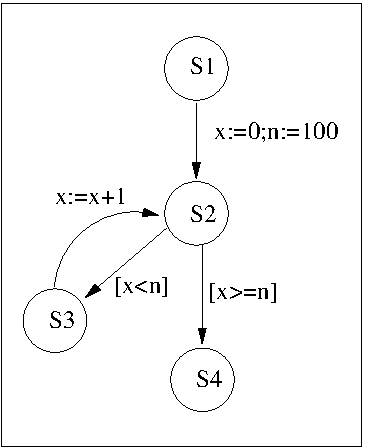
\includegraphics{figures/chap04/example1.pdf}
	\end{minipage}
	%
	\begin{minipage}{.5\textwidth}
		\centering
		\begin{lstlisting}
		int x,n;
		x=0;
		n=100;
		while(x<n)
			x=x+1;
		\end{lstlisting}
	\end{minipage}
	\caption{示例程序及其控制流图}
	\label{fig-example}
\end{figure}


控制流图存在其他的变种,例如编译器LLVM/Clang定义的控制流图将指令放在节点中。
但是,它们所定义的程序语义是等价的。程序的语义通常由状态迁移系统定义。

\begin{definition}
一个状态迁移系统可以定义为一个三元组$T=(S, R, S_0)$,其中,$S$是所有可能状态的集合(也称为状态空间);$R \subseteq S \times S $是迁移关系集合;$S_0$是初始状态集合。
\end{definition}


程序的状态空间由两部分构成:程序指令的位置和程序变量的取值。
给定程序变量集合$Var$,用符号$\textbf{Var}$表示变量所有可能取值集合,
那么,程序的状态空间可以表示为$S = L \times \textbf{Var}$,
其中,$L$是程序控制流图中的控制节点集合。
程序的状态空间可能是有穷集合,也可能是一个无穷集合,
如程序中含有整型变量时,其可能的取值范围为所有整数集合。
同理,程序的初始状态可能有无穷多个,如变量未初始化时。

迁移关系$R$定义了程序的进行一步操作时的状态变化过程,例如,
在图\ref{fig-example}所示程序中,
迁移$((S1, x=*, n=*), (S2, x=0, n=100))$
表示了程序在$S1$位置处执行赋值操作后,变量赋予相应的取值,
其中,符号$*$表示变量的取值为任意值。

一般地,程序的执行可以用一个迁移序列表示,例如,序列
$((S1, x=*, n=*), (S2, x=0, n=100),
(S3, x=0, n=100), (S2, x=1, n=100),
(S3, x=1, n=100) )$表示图\ref{fig-example}
中的程序从初始状态执行,并进入一次循环的状态变化过程。
为表述方便,本节用符号$r\in R$表示一个迁移,序列$r_0 r_1 \cdots r_n$表示一条迁移序列。

一个状态是可达的,当且仅当存在一条执行路径,使得程序能够从初始状态运行到达该状态。
形式化地,状态$s\in S$是可达的,当且仅当存在迁移序列$r_0 r_1 \cdots r_n$,
其中 $r_n = (s_n, s_{n+1})$,使得$s_0$为初始状态,且$s = s_{n+1}$。

给定一些错误状态,或者不安全的状态,
检测程序是否安全的问题可以归结为检测这些错误状态是否可达的问题,
即是否存在一条执行路径,使得程序能够从初始状态执行到某些错误状态。
因此,本质上,程序安全性分析问题可以归结为程序的可达状态空间遍历问题,
即通过遍历程序的所有可能状态空间,检测是否存在不安全的状态。


\subsection{程序不动点语义}

程序的可达状态集合通常是通过计算程序语义泛函的最小不动点得到。
该语义泛函是定义在程序状态迁移系统上的$Post$后继算子。


\begin{definition}
给定状态迁移系统$T=(S,R,S_0)$,
后继算子$Post: S \times R \rightarrow S$
是一个从状态空间和迁移关系到状态空间的映射。
给定状态集合$S_1 \subseteq S$,
$Post(S_1, R) = \{ s\in S | \exists s_1 \in S_1 \wedge (s_1, s)\in R \}$。
\end{definition}

与控制流图类似,后继算子也存在其他变种定义。
在程序分析中,后继算子通常也定义为从状态空间和程序指令到状态空间的映射,
即$Post: S \times Expr(Var, Func) \rightarrow S$。
通过将程序指令进行符号化编码(symbolic encoding),上述两个定义是等价的。
为表述方便,对上述两种定义不做区分。

直观上,给定程序的当前状态和迁移关系,
$Post$算子定义了在下一时刻,程序从当前状态执行一步迁移可能到达的状态集合。

$Post$后继算子作用在状态集合上。
一个状态集合称为程序语义的具体域中的一个元素。
因此,$Post$算子也可以看做是程序语义的具体域上的函数。
给定程序变量集合$Var$,以及变量可能取值集合$\textbf{Var}$,
程序的具体域为幂集$2^{\textbf{Var}}$。
可证后继算子是该具体域上的单调递增函数。

\begin{lemma}
$Post$后继算子是单调递增函数。
\end{lemma}

\begin{proof}
	假设状态集合$S_1 \subseteq S_2 \subseteq S$,
	证明义务为$Post(S_1, R) \subseteq Post(S_2,R)$。
	
	依据$Post$后继算子的定义,
	$Post(S_1, R) = \{ s\in S | \exists s_1 \in S_1 \wedge (s_1, s)\in R \}$,
	那么对任意$s\in Post(S_1, R)$,
	存在$s_1\in S_1$,使得$(s_1, s)\in R$。
	依据假设$S_1 \subseteq S_2$,得知$s_1 \in S_2$,
	故$s\in Post(S_2, R)$。
\end{proof}


一般地,从程序的初始状态,执行$n$次$Post$后继算子,
将得到程序执行$n$步可能到达的状态空间。
理论上,程序的可达状态空间可以通过$Post$后继算子进行数学刻画:
$Reach = \bigcup_{i=0}^{\infty}\{Post^{i}(S_0, R)\}$,
其中,$S_0$是程序的初始状态集合。
程序的可达状态空间可以通过不断迭代运用$Post$后继算子,
直至得到所有可能状态。
然而实际情况下,该迭代计算是不收敛的。
假设上述计算在迭代$n$次后终止,
表示程序的所有可达状态可以在$n$步计算内穷举,
第$n+1$计算不会产生新的状态,即$Post$算子存在不动点。


\begin{lemma}
程序的可达状态空间$Reach$等价于程序语义泛函$Post$算子的最小不动点,
即$Reach = LFP(Post)$。
\end{lemma}

由Knaster-Tarski不动点定理可知,	完备格上的单调函数存在最小不动点。
因此,如果程序语义的对象域构成一个完备格,并且程序的语义泛函是一个单调函数,
那么程序语义的最小不动点一定存在。
然而,即便理论上存在最小不动点,
该迭代过程的计算复杂度也随着程序规模的增长而呈指数级增长。
这就是通常所说的状态空间爆炸问题。

\section{动态符号执行技术}
%动态测试用例生成技术从2005年开始兴起,又被称为白盒Fuzzer。该技术以
%一组随机生成的数据作为输入,通过分析程序动态执行信息来获取可达路径对输
%入数据的约束,并在遇到受输入数据控制的分支跳转时将收集到的约束,输出至
%可满足模求解器(SMT Solver),用以判定另一分支路径是否可达。若可达,求解
%器则给出覆盖目标分支路径的测试用例,并利用生成的测试用例发掘目标分支路
%径中的软件缺陷。典型系统包括微软研究院的 DART\upcite{godefroid_dart:_2005}、 SAGE\upcite{godefroid_sage:_2012}、SmartFuzz\upcite{molnar_dynamic_2009}、 Hunter\upcite{hunter__2010}等。

%动态测试用例生成技术主要目标有两点:(1)为待测程序单元自动的生成可
%达到较高覆盖率的测试数据;(2)在动态过程中寻找待测程序的缺陷。

%作为动态测试用例生成技术的前身,传统的符号执行技术使用符号变量代替
%待测程序单元的实际输入值,之后使用替代的程序执行语义模拟执行待测程序单
%元。在执行过程中遇到的包含符号变量的条件表达式即为可决定程序执行路径的
%路径约束。待测单元的所有路径可通过对路径约束的真值赋值表示为一棵二叉执
%行树,其中每一个内部节点代表了一个分支路径选择。通过在树上深度优先的回
%溯搜索,寻找、判定预期路径约束的可达性并寻找对应的数据样本,满足预期执
%行路径的实际输入值即可被产生。但是,这种传统方法在处理大规模的或者较为
%复杂的待测单元时存在问题。例如,如果某一个路径约束的可满足性是无法判定
%的,那么传统的符号执行技术就无法继续进行搜索,从而导致了不佳的覆盖率;
%对于包含复杂数据类型(例如指针、数组)的程序,依靠静态的模拟执行无法精
%确的求解路径约束,同样也会在真实测试中导致低覆盖率。

动态测试用例生成技术的提出正是为了解决传统方法的不足,其基本想法在
于将传统符号执行中的符号输入与具体值输入相结合。动态符号执行采用实际输
入值真实地执行待测程序单元,在程序执行的过程中进行符号执行过程构建路径
约束,同时记录通过符号变量表达的抽象程序状态,以及用实际数值表达的真实
程序状态。由于待测程序被真实的执行了,所以所收集到的路径约束是遵循程序
本身的语义的,且是精确的。因而在动态方法中不会出现如静态方法的虚假警报,
并且也有助于对复杂数据结构进行分析处理。另外,由于程序的真实状态被记录,
一旦遇到不可判定的路径约束,可使用变量的实际值替代符号值,使后续的路径
探索过程可以继续进行。因为相比传统方法,可达到更高的覆盖率,所以其被广
泛的应用在了程序测试与验证中,并且有相当多的工作扩展了动态符号执行的适
用范围,如通过引入额外的内存模型以更精确的处理数组;通过引入额外的分析
方法提高对循环的覆盖率等。

动态测试用例生成技术的一般流程如图\ref{动态符号执行流程}所示。 其处理流程如下:
\begin{enumerate}[(1)]
\item 以某一具体输入启动目标程序, 该输入可随机生成;
\item 在目标程序的地址空间中,将输入对应的机器位置标记为符号变元;
\item 对目标程序的每条指令,将其计算语义提升到基于符号变元的符号表达式
域下,计算其抽象语义,更新对应的符号机器状态。对于符号计算相关的流程转
移类的指令,计算其对应于当前具体执行路径的分支谓词,累积至当前路径对应
的全局约束条件,同时计算另外一条分支对应的符号约束,通过约束求解进行可
满足性判断,确定该路径的可行性。在可行的情况下,将分支对应的路径约束保
存入调度队列;
\item 若调度队列非空,则从调度队列中抽取出一个分支约束,计算出满足约束
条件的输入的具体值,回到步骤 ① 对该路径进行符号分析;否则,即结束对目
标程序的符号分析。
\end{enumerate}

\begin{figure}[h]
\begin{center}
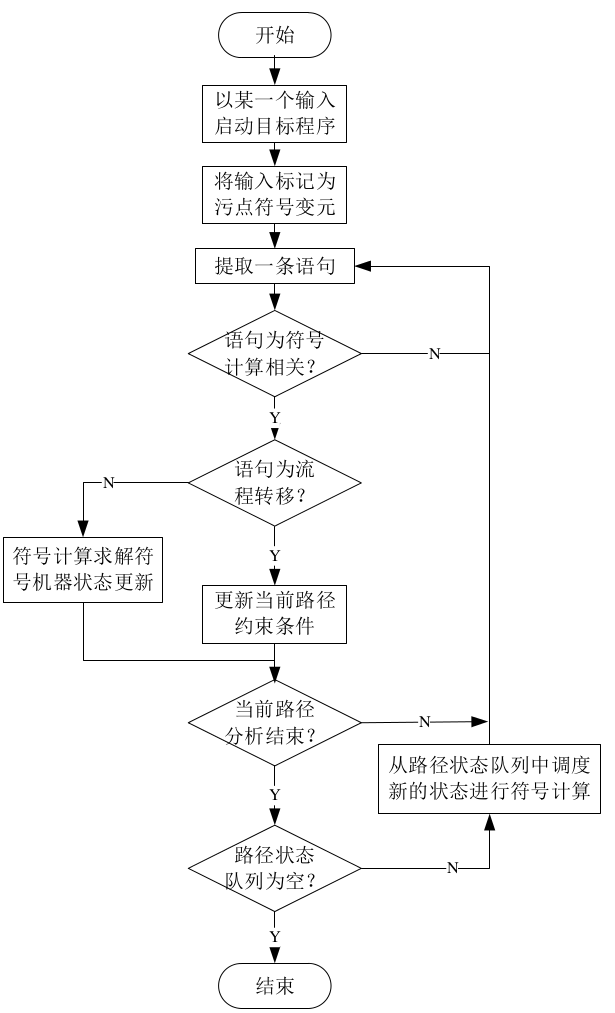
\includegraphics[scale=0.4]{chap02/动态符号执行流程}
\end{center}
\caption{动态符号执行流程}
\label{动态符号执行流程}
\end{figure}

论文第五章使用的符号执行工具是KLEE\upcite{cadar_klee:_2008}。KLEE是由Cadar与2008年开发的动态符号执行工具。KLEE依托于LLVM编译器,支持的最高的LLVM版本是3.4。KLEE执行LLVM字节码,记录程序中不同的路径,使用运行时检查器(Runtime Checker)检测程序错误,并利用约束求解器求解路径约束产生测试用例。KLEE能够获取很高的代码覆盖率并且发现深层次漏洞。

KLEE的架构如图\ref{KLEE架构}所示。和很多其他的符号执行工具一样,KLEE包含的一个主要的组件是metaSMT接口,支持多种约束求解器,例如Z3,STP,Boolector。KLEE还包含多种搜索策略即深度优先、宽度优先、随机搜索、最大覆代码覆盖率以及混合搜索策略,且提供了基本的搜索策略接口,可以方便的自定义搜索接口。此外,KLEE还实现了环境交互模型,即利用自己编写的数据读写函数代替程序原始调用的函数,例如open,read等。此做法有三个好处:(1)简化版的函数能够减轻原始复杂程序造成的路径爆炸;(2)能够根据代码规范模拟闭源的代码库,使得符号执行能够顺利执行;(3)通过模拟网络通信可以符号执行网络程序。尽管环境建模有这些优点,但是程序的模拟代码都是使用者手动编写的,每次遇到不同的程序需要重新编写。

\begin{figure}[h]
\begin{center}
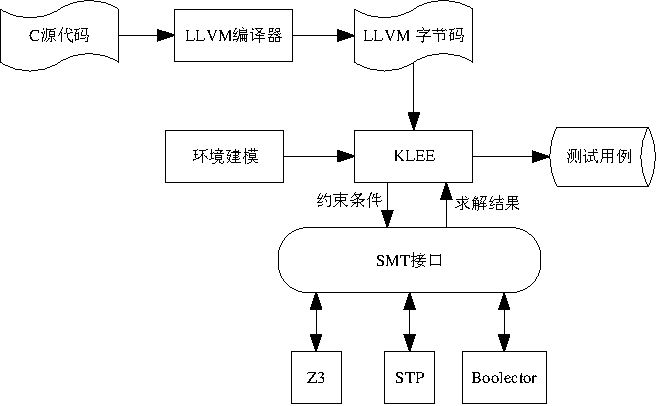
\includegraphics[scale=1.2]{chap02/KLEE架构}
\end{center}
\caption{KLEE架构}
\label{KLEE架构}
\end{figure}


%抄wb
%\section{模糊测试}
%模糊测试是指通过不断给目标软件发送各种畸形数据来挖掘其中可能隐含的
%安全漏洞,是一种强制性的漏洞挖掘方法。模糊测试与传统白盒方法不同,不需
%要分析程序源代码;也与传统黑盒测试只关注用例输出是否与预期相符有所不同,
%模糊测试只关注目标软件是否出现了异常\upcite{sutton_fuzzing:_2007}。
%
%\subsection{模糊测试的一般过程}
%具体模糊测试方法根据目标软件、输入格式、运行平台等不同的测试需求各
%不相同,但基本过程是一致的,包括以下几个步骤:
%
%(1)确定输入向量
%
%由于可利用漏洞都是由于软件在处理用户输入时没有经过正确的校验。因此,
%输入向量的枚举是模糊测试方法取得成功的关键因素。所有软件能够接收的数据
%都应该被认为是输入向量的组成部分,主要包括文件输入、网络数据包等。
%
%(2)生成测试用例
%
%在了解输入特性后,就可以根据变异或随机构造的方式生成测试用例。根据
%目标软件及其数据格式的不同,用例的生成方式也各不相同,可以采用随机生成
%的方式,也可以采用基于正常样本变异的方式,或者采用启发式规则生成的方式
%等\upcite{robertson_run-time_2003} 。一般模糊测试系统会生成海量测试用例,而其中大部分的用例都是无效
%的。因此,一般需要深入分析目标软件,构造更加有效的用例。
%
%(3)执行测试用例
%
%这一步通常与用例生成并行进行,执行过程一般包括启动目标软件、适用测
%试用例激励目标软件等。
%
%(4)异常检测与分析
%
%尽可能多地触发软件异常是模糊测试的目标。因此在测试目标软件时,应实
%时监测一切可能的异常、崩溃等信息,在异常发生时记录和保存重要的运行状态
%信息。并进一步分析软件异常的可利用性,合并重复的异常信息等。
%
%\subsection{测试用例生成方法}
%
%模糊测试是一种试图遍历软件输入空间的方法。因此,测试用例生成方法的
%好坏是影响模糊测试有效性的重要因素。测试用例生成方法大体上可分为两大类:
%基于变异的方法和基于生成的方法。
%
%(1)基于变异的方法
%
%这种方法从一个有效的输入样本开始,随机地变异样本中的部分数据来生成
%新用例。这是一个比较原始的方法,几乎不需要被测软件的任何先验知识,实现
%起来非常简单且通用性强。但这种方法效率很低,因为被测软件浪费了大多数的
%时间处理无效的输入数据。因此,后续有很多改进的方法,比如基于静态分析辅
%助的方法\upcite{wu_new_2009,lanzi_smart_2007,rawat_offset-aware_2011},基于运行时反馈方法 \upcite{ganesh_taint-based_2009,bekrar_finding_2011},基于遗传算法的方法\upcite{rawat_evolutionary_2010,liu_vulnerability_2008,cordon_ten_2004} 等。
%
%(2)基于生成的方法
%
%随机生成是最简单的生成策略,该方式只是简单地产生大量伪随机数据用于
%激励目标软件,能否触发异常有很大的概率性。因此,此法虽然简单却并不常用。预生成测试用例也是一种常见的生成策略,该方式首先研究目标软件的输入
%规范说明,以了解其支持的输入数据结构和取值范围,然后生成硬编码的畸形数
%据以测试边界条件或违反规约\upcite{liubiao__2014} 。这种方式生成的用例针对性强,因此测试效
%率相对较高。但是,创建这些用例需要事先完成大量的分析工作,自动化程度不
%高,而且有的输入规范并不可得。还有一种就是基于符号执行的生成方法,如
%SmartFuzz\upcite{molnar_dynamic_2009} 、SAGE\upcite{godefroid_sage:_2012} 等,这些系统将正常测试数据当作符号值,收集目标软件
%处理正常输入时的路径约束,通过约束求解生成新用例。理论上符号执行的方式
%能够生成精准的用例,但实际测试过程中由于面临路径爆炸、分析精度受限、指
%针分析难等问题,其应用场景也受到限制。
%
%\subsection{模糊测试框架}
%
%模糊测试框架是模糊测试过程的通用化实现。通过使用测试框架可以简化被
%测软件输入的表达、被测目标的监测和异常分析管理等,能够极大地提高模糊测
%试的自动化水平。虽然已经存在很多模糊测试框架,比如antiparser\upcite{noauthor_antiparser_nodate} 、
%Peach\upcite{noauthor_peach_nodate} 、Sulley\upcite{noauthor_sulley:_2017}、AUTODAFE\upcite{noauthor_autodafe_nodate} 等,但它们并不提供通用的解决方案,有其
%特定的适用范围。一般来讲,使用模糊测试框架可以实现功能复用,便于经验的
%积累和分享;但同时也必须花大量时间来学习框架,某些测试功能还可能因为框
%架的限制而无法实现。
%虽然模糊测试缺乏形式化模型和理论基础,然而模糊测试却是迄今为止发现
%未公开漏洞数量最多的挖掘方法。模糊测试实际上利用了漏洞挖掘问题的可猜解
%性和可验证性,虽然无法准确回答是否能检测到漏洞、是否能检测出所有漏洞等
%问题,却能够挖掘出很多意想不到的漏洞。因此,在其他挖掘方法效果不理想时,
%模糊测试可以作为一种很好的补充手段。论文在分析可编程类软件时,就采用了
%模糊测试的思想,基于模糊编程的思路对被分析软件进行测试。
%%抄wb

%\section{基于机器学习的漏洞检测方法}



\section{本章小结}

本章介绍了源代码漏洞挖掘中所使用的四种中间表示:语法分析树、抽象语法树、控制流图以及数据流图。在分析了各类中间表示表达能力的基础上,根据需要的中间表示数量的不同,将源代码软件漏洞描述为三类,即基于抽象语法树的源代码漏洞描述、基于控制流的源代码漏洞描述以及基于污染传播的源代码漏洞描述。最后,介绍了第五章所使用的静态程序分析基础以及动态符号执行技术。

\chapter{基于程序性质图的源代码软件漏洞挖掘方法研究}

根据Rice定理\upcite{rice_classes_1953},通过一个程序完全的自动检测其他程序的复杂属性是不可行的。
一般的源代码静态分析工具都是基于字符串匹配或者抽象语法树匹配的,
所以现行的工具要么局限于特定类型的漏洞,要么需要大量的人工审计工作\upcite{heelan_vulnerability_2011}消除误报。例如PREfast\upcite{bush_static_2000}、RATS\upcite{wnoauthor_cern_nodate}以及PScan\upcite{dekok_pscan:_2000}虽然能够检测一些程序开发过程中产生的漏洞,但是很难检测成因复杂的漏洞。而另外一些工具,例如Splint\upcite{noauthor_splint_nodate}只能检测特定的漏洞。

%审计像Linux内核这样具有庞大代码量的软件系统是一件不可能完成的事情。基于动态测试的方法,例如模糊测试和符号执行,虽然能够挖掘不同类型的漏洞而且能够产生测试用例,但是符号执行随着软件规模的增加会出现路径爆炸问题,此外符号执行还有交互环境模拟问题以及约束求解器求解能力的限制问题;模糊测试则存在随机性强,代码覆盖率低的问题。所以,首先漏进行洞可疑区域标定然后再动态测试可疑区域是一个解决办法。

针对C/C++源代码软件,本章提出了一种基于程序性质图的源代码漏洞挖掘方法。该方法利用程序性质图聚合抽象语法树、控制流图、数据流图三种中间表示,通过定义以及组合不同的程序性质图遍历方式能够检测多种源代码软件漏洞。
%对于缓冲区溢出漏洞,影响漏洞的特征有很多种,漏洞的形成是多个特征综合作用的结果。
针对缓冲区溢出漏洞挖掘精确度不高的问题,
本章提出了一种基于机器学习的缓冲区溢出漏洞挖掘方法。该方法首先将缓冲区溢出静态特征分成7类;然后,在已标记的漏洞中,利用扩展的程序性质图获取静态特征并将其映射到向量空间,作为机器学习算法的训练集;最后,选取5种有监督机器学习算法在训练集中训练分类器,并通过分类器在新的源代码中挖掘缓冲区溢出漏洞。

\section{程序性质图生成}\label{程序性质图生成}

程序性质图(Code Property Graph,CPG)是源代码在性质图(Property Graph,PG)\upcite{rodriguez_graph_2010}上的表现形式。本节介绍了性质图的概念、各种中间表示的生成过程、程序性质图以及程序性质图的各种遍历方式。

\subsection{性质图}

在图理论当中,有向图可以用一个关系对表示,$G=(V,E)$,$V$是节点集合,$E\subseteq(V \times V)$是节点之间边的集合。性质图的节点具有以下特性:{(1)}每个节点都对应一个唯一标识符;{(2)}每个节点都包含一个入边和出边集;{(3)}每个节点都包含键-值集。性质图的边具有相似的性质:{(1)}每条边对应一个唯一标识符;{(2)}每条边都包含一个标签表示边的类型;{(3)}每条边都有一个键值集;{(4)}每条边都有一个源节点和目的节点。图\ref{性质图示意图}展示了上述特性。

%\textbf{下面的图删除,}

\begin{figure}[htp]
\centering
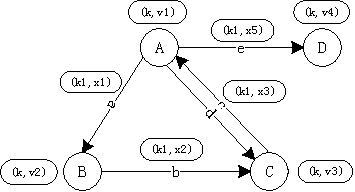
\includegraphics[scale=1.5]{性质图示意图}
\caption{性质图示意图}
\label{性质图示意图}
\end{figure}


\begin{definition}
 \label{性质图定义}
 性质图$G=(V,E,\lambda ,\mu, s,d)$是一个有向的、边标记的、属性化的多重图,$V$是节点的集合,$E$是有向边的集合,$s: E \rightarrow V$和$d:E \rightarrow V$分别是有向边到源节点和目的节点的映射,$\lambda : E \rightarrow \sum $是边标记函数,将一条边映射到字符集$\sum$中的一个字符。节点和边都用键—值对表示性质,性质的赋值函数为$\mu:(V \cup E) \times K \rightarrow S$,$K$和$S$分别是性质的键和值。
\end{definition}

源代码软件漏洞分析依赖于多种代码的中间表示例如语法分析树、抽象语法树、数据流图、控制流图等,对于C/C++,很多编译器的前端能够很容易的通过插桩的方式生成中间表示。但是当分析涉及到复杂的程序或者跨越多个程序搜集中间表示时,编译程序所需要的环境就很难得到保证,特别的是,一般的编译器前端无法处理代码有头文件缺失的情况。与源代码相关的中间表示都直接或者间接的建立在语法分析树的基础上,所以程序性质图的生成首先需要将源代码转换成语法分析树。在语法分析树的基础上生成抽象语法树、控制流图、数据流图,然后将各种中间表示合并为一个统一的表示形式——程序性质图,然后将程序性质图存入图数据库,用查询的方式搜索节点和边。程序性质图的生成过程如图\ref{程序性质图生成过程}所示。

\begin{figure}[htp]
\centering
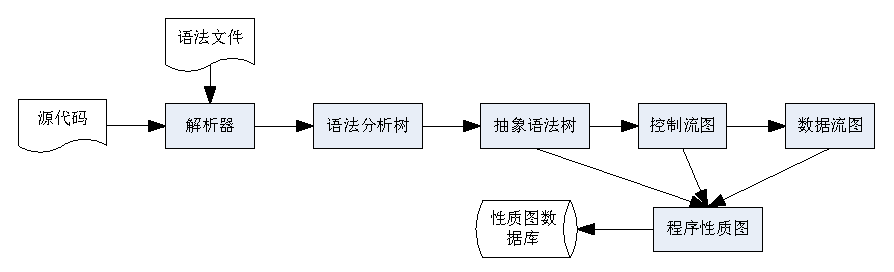
\includegraphics{chap03/程序性质图生成}
\caption{程序性质图生成过程}
\label{程序性质图生成过程}
\end{figure}

\subsection{鲁棒的源代码中间表示生成}
\label{源代码的鲁棒分析}
鲁棒的源代码中间表示生成顺序依次是语法分析树、抽象语法树、控制流图、数据流图。语法分析树建立在ANTLR\upcite{parr_definitive_2013}{(ANother Tool for Language Recognition)}的基础上。ANTLR是一种非常强大的用于读取、执行或者翻译结构性的文本以及二进制文件的解析器生成器,广泛的应用于构建编程语言解析器、工具和框架上。对于C/C++,基于岛屿语法{(Island Grammar)},可以利用ANTLR实现三个层次上的语法解析器:分别是模块解析器、函数解析器以及语句解析器。模块解析器解析粗略的结构信息,例如函数、命名空间以及全局的变量声明。函数解析器解析辨别函数内部能够影响到程序控制流的程序结构,例如跳转语句goto、continue和break;选择语句,如if语句、switch语句;循环语句,如for循环、while循环和do-while循环。语句解析器主要的作用是将任意一个语句分解为表达式、操作符以及标识符等。岛屿语法\upcite{moonen_generating_2001}是一种定义文本结构的语言,通过此语法可以定制解析器的粒度。

图\ref{模块解析器的岛屿语法片段}是模块解析器的岛屿语法片段,第一行中的module表示一个模块,function\_def表示一个函数,simple\_decl表示变量或者类的声明,water表示其他的任意未定义字符,图\ref{模块解析器的岛屿语法片段}表达的意思是一个module可以由一个或者多个functionDef、simple\_decl、using\_directive或者water组成。图\ref{函数解析器的岛屿语法片段}是函数解析器的岛屿语法片段,表示函数有哪些元素组成,其中template\_declStart,return\_type,function\_name,compound\_statement分别表示函数模板、函数返回类型、函数名以及函数内容。图\ref{语句解析器的岛屿语法片段}是语句的岛屿语法片段,第一行表示statements可以由条件编译标识符{(pre\_opener,pre\_closer,pre\_else分别表示\#if,\#endif和\#else)}和语句statement构成。statement的组成当中最主要的是simple\_decl和expr\_statement。expr\_statement是C/C++作为程序主体的每一行代码,在岛屿语法中需要按照运算符的优先级、结合进行设计{(14-17行)}。解析器按照语法文件上规定的顺序解析程序中的非终结符,其他的未被制定的终结符和非终结符用water表示。

\begin{figure}[h]
\begin{lstlisting}[language=C]
module : (function_def | simple_decl | using_directive | water)*;
using_directive: USING NAMESPACE identifier ';';
simple_decl : (TYPEDEF? template_decl_start?) var_decl;
...
water : any_token
\end{lstlisting}
\caption{模块解析器的岛屿语法片段}
\label{模块解析器的岛屿语法片段}
\end{figure}

\begin{figure}[h]
\begin{lstlisting}[language=C]
function_def : template_declStart? return_type? function_name function_paramList ctorList? compound_statement;
template_decl_start : TEMPLATE '<' template_param_list '>';
...
returnType : (functionDeclSpecifiers* typeName) ptrOperator*;
...
function_param_list : '(' parameter_decl_clause? ')' CV_QUALIFIER* exception_specification?;
parameter_decl_clause: (parameter_decl (',' parameter_decl)*) (',' '...')? | VOID;
parameter_decl : param_decl_specifiers parameter_id;
...
function_name: '(' function_name ')' | identifier | OPERATOR operator;
...
compound_statement: opening_curly (statements) closing_curly;
...
\end{lstlisting}
\caption{函数解析器的岛屿语法片段}
\label{函数解析器的岛屿语法片段}
\end{figure}

\begin{figure}[h]
\begin{lstlisting}[language=C]
statements: (pre_opener | pre_closer | pre_else | statement)*;
statement: opening_curly
         | closing_curly
         | block_starter
         | jump_statement
         | label 
         | simple_decl
         | expr_statement
         | water;
...
expr_statement: expr? ';';
expr: assign_expr (',' expr)?;
assign_expr: conditional_expression (assignment_operator assign_expr)?;
conditional_expression: or_expression
		      | or_expression ('?' expr ':' conditional_expression)
or_expression : and_expression ('||' or_expression)?;
and_expression : inclusive_or_expression ('&&' and_expression)?;
...
\end{lstlisting}
\caption{语句解析器的岛屿语法片段}
\label{语句解析器的岛屿语法片段}
\end{figure}

输入一个程序,解析器根据语法文件辨别每一个终结符和非终结符,将这些标识符连接之后会得到语法分析树。语法分析树能够展示编程语言元素的类别、结构以及相互之间的关系.语法分析树是上述解析器输出的唯一表示形式,它忠实的按照语法文件解释源代码的结构细节,其表现形式较为冗余且对微小改动非常敏感。ANTLR内置了生成语法分析树的功能。以第二章图\ref{一个简单的实例程序}为例,生成的语法分析树如图\ref{抽象语法树示意图}所示。

抽象语法树能够直接从语法分析树生成,与语法分析树相比,抽象语法树删除了对程序没有影响的实现细节,更加注重代码的结构,是一种更为紧致简明的中间表示形式也更加的适合于源代码的分析。图\ref{抽象语法树示意图}是图\ref{一个简单的实例程序}的抽象语法树的示意图。抽象语法树能够松的定位和检测程序中的每一行代码以及每行代码中的变量、变量类型操作符等信息,但却不适用于检测代码的执行顺序,所以需要程序的控制流图来展示程序语句的执行顺序以及控制条件。

在辨别程序跳转关键词的基础上,程序的控制流图可以从抽象语法树直接生成,常见的关键词有$if$,$for$以及$goto$。根据这些信息,可以使用以下两步将抽象语法树转换成控制流图。首先,在过程内顺序连接抽象语法树中的语句节点,定义$if$,$for$以及$while$语句转换为控制流图的方式并在所有的抽象语法树上使用此规则;然后处理$break$,$continue$以及$goto$等跳转语句矫正控制流图。实际上,第二阶段仅仅在控制流图上加入了由跳转语句引入的额外的边。图\ref{控制流图}是图\ref{一个简单的实例程序}的控制流图。

每一个程序语句可以使用(use)或者定义(define)变量。如果语句$s2$使用了$s1$定义的变量$v$,且从$s1$到$s2$存在一条路径上,$v$在这条路径中未被重定义,则称$s2$数据依赖于$s1$。将具有数据依赖关系的程序语句使用数据流边连接起来则形成程序的数据流图。图\ref{程序数据流图}是图\ref{一个简单的实例程序}的控制流图。
%\begin{figure}[htp]
%\centering
%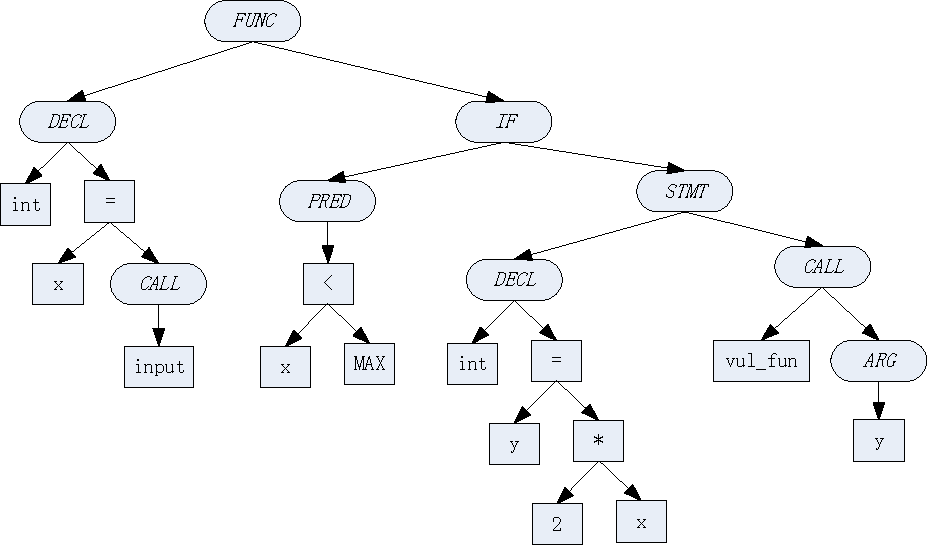
\includegraphics{抽象语法树示意图}
%\caption{Listing \ref{一个简单的实例程序}抽象语法树示意图}
%\label{抽象语法树示意图}
%\end{figure}



%\begin{figure}[htp]
%\centering
%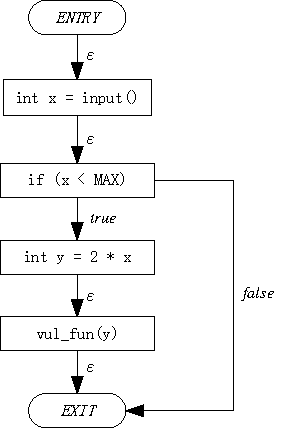
\includegraphics{控制流图}
%\caption{Listing \ref{一个简单的实例程序}控制流图}
%\label{控制流图}
%\end{figure}

%在分析源代码上的漏洞时需要跟踪数据的流向以判断目标语句是否输入可控,这是漏洞是否可利用的一个重要判断依据,与此同时也需要判断目标语句在控制流上是否可达,所以在此引入数据流图。数据流图原本仅仅用于程序切片,现在则成为一个通用的分析数据流以及谓词在程序执行中的作用的工具。数据流图将每个程序语句和谓词都看做一个节点,展示语句和语句之间的数据交互关系。
%\textbf{参考数据依赖和控制依赖的定义来写,不要用那个图}

%\textbf{数据依赖。}程序的每一条语句$s$都会使用{($use$)}或者定义{($define$)}变量。$s$定义了$v$是指$s$将一个值赋给了$v$,这里$s$可以是一个赋值语句也可以是一个输入语句。$s$使用了$v$是指$s$中引用了$v$,例如$v$出现在赋值语句$s$的右半部分,$s$还可以是返回语句、条件语句或者循环语句中的谓词。可以这样定义$use$和$define$操作,$use(s)=\{v | v\text{是}s\text{使用的变量}\}$,$define(s)=\{v | v\text{是}s\text{定义的变量}\}$。语句$s$数据依赖于$use(s)$中的所有变量,定义这些变量的语句和$s$形成数据依赖关系。将所有具有依赖关系的节点连接,则形成数据流图,如图\ref{数据流图}所示。

%\textbf{控制依赖。}一个语句是否能够执行有时会依赖谓词的值,例如Listing \ref{一个简单的实例程序}中vul\_fun(y)执行的条件是谓词x<MAX的值是true。控制依赖关系可以通过控制流图和支配树获取。
%
%Listing \ref{一个简单的实例程序}的控制依赖图如图\ref{数据流图}所示。数据流图打乱了程序节点在控制流图上的顺序,通过给边增加属性值的方式表示数据、控制依赖关系。图中最上层的节点是变量x的定义节点,if语句中的谓词x<MAX使用了变量x并且支配了变量y的定义语句,vul\_fun函数受if语句支配并且使用了变量y。

%\begin{figure}[htp]
%\centering
%\includegraphics{数据流图}
%\caption{Listing \ref{一个简单的实例程序}数据流图}
%\label{数据流图}
%\end{figure}

\subsection{程序性质图}\label{程序性质图}

由于不同种类的源代码软件漏洞具有不同的特征,现存的基于模式匹配的漏洞挖掘工具,一方面不能检测多种源代码软件漏洞,另外一方面则会造成很高的误报,所以需要一种综合的表示形式{——}程序性质图(Code Property Graph, CPG)。
%\upcite{yamaguchi_modeling_2014, yamaguchi_automatic_2015}。
程序性质图可以通过存入专门的图数据库,例如Neo4j\upcite{noauthor_neo4j_nodate},Titan\upcite{noauthor_titan:_nodate}和OrientDB\upcite{noauthor_newsletter_nodate},然后利用数据库查询的方式对程序语句节点以及语句节点之间的关系进行查询。程序性质图是一个抽象语法树性质图、控制流性质图和数据流性质图的综合表示。本节分别定义了三类中间表示的性质图表现形式,然后在此基础上定义程序性质图。

\begin{definition}
\label{抽象语法树定义}
抽象语法树性质图$G _{A}=(V_{A},E_{A},\lambda _{A}, \mu _{A}, s _{A}, d _{A})$,$V_{A}$是抽象语法树节点的集合,$E_{A}$是边集合,$\lambda _{A}$是边的标签函数,用任意字符标记每一条边,$s _{A}$和$d _{A}$是边到节点的映射,分别将边映射到源节点和目的节点。
\end{definition}

抽象语法树节点的性质包括:节点类型{(type)}、代码{(code)}、节点序号{(childnum)}、操作符{(operator)}、位置{(location)、所属文件{(file)}是否控制流节点{(isCFGNode)}。图\ref{抽象语法树性质图实例}为图\ref{一个简单的实例程序}的生成的部分抽象语法树性质图实例。

\begin{figure}[htp]
\centering
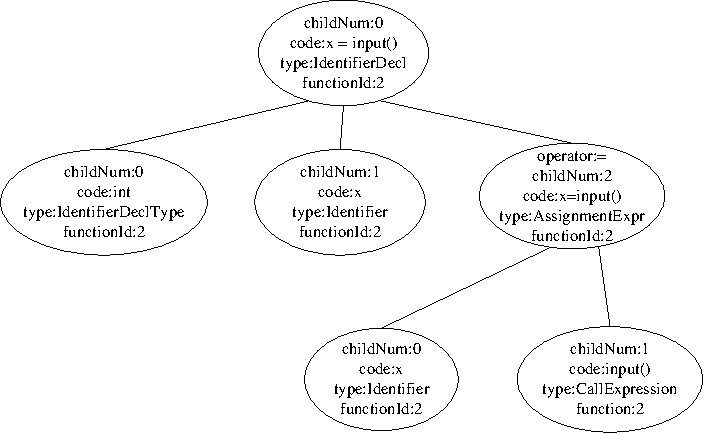
\includegraphics{chap03/抽象语法树性质图实例}
\caption{抽象语法树性质图实例}
\label{抽象语法树性质图实例}
\end{figure}

\begin{definition}
\label{控制流性质图定义}
控制流性质图可以用$G _{C}=(V_{C},E_{C},\lambda _{C}, \mu _{C}, s _{C}, d _{C})$表示,其中$V_{C}=\{ \upsilon | \upsilon \in V_{A} \cup \{ENTRY,EXIT\},\text{且} 对于每一个节点有\mu_C(isCFGNode, type)=True \}$,其中$ENTRY$和$EXIT$是控制流性质图的入口节点和结束节点,$E_{C}$是边的集合,标签函数$\lambda_C$将边映射到字符集 $\sum_C=\{true, false, \epsilon \}$,$true$和$false$用于标记$Condition$语句的两种出边,$\epsilon$用于表示其他没有控制流跳转的边。
\end{definition}

图\ref{控制依赖性质图实例}是图\ref{一个简单的实例程序}的控制依赖性质图的一部分(删除了$ENTRY$节点),从图中可以看出所有节点的$isCFGNode$属性都为$True$。

\begin{figure}[htp]
\centering
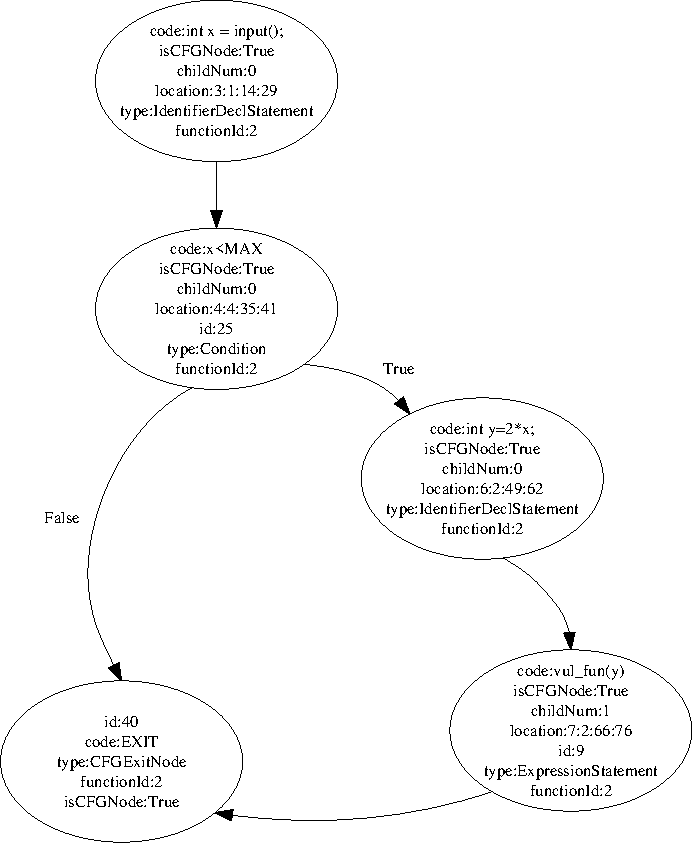
\includegraphics[height=18cm]{chap03/控制依赖性质图实例}
\caption{控制依赖性质图实例}
\label{控制依赖性质图实例}
\end{figure}

\begin{definition}
\label{数据依赖性质图定义}
数据依赖性质图可以用$G _{D}=(V_{D},E_{D},\lambda _{D}, \mu _{D}, s _{D}, d _{D})$表示,其中$V_{D} \subseteq V_C \subseteq V_A$,$E_{D}$是边的集合,标签函数$\lambda_{D} : E_{D} \rightarrow \sum_{D}$,$\sum_{D} = \{D\}$,其中$D$表示数据依赖,同时在表示数据依赖关系的边上增加一个属性$symbol$表示传递的标识符。
\end{definition}

图\ref{数据依赖性质图实例}是图\ref{一个简单的实例程序}的数据依赖图的一部分,此图的节点是是控制流依赖图节点的子集,每条边都有symbol属性表示传递的数据。

\begin{figure}[htp]
\centering
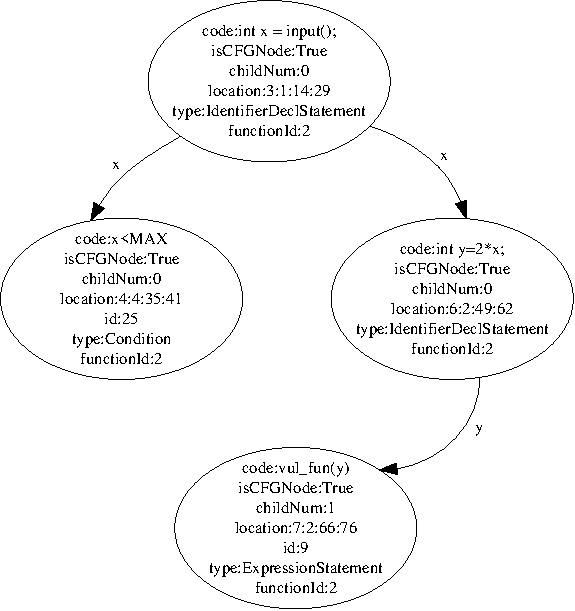
\includegraphics{chap03/数据依赖性质图实例}
\caption{数据依赖性质图实例}
\label{数据依赖性质图实例}
\end{figure}

通过聚合上述三种性质图的定义,可以获得程序性质图的定义如\ref{程序性质图定义}所示。

\begin{definition}
\label{程序性质图定义}
程序性质图可以用$G=(V,E,\lambda, \mu, s, d)$表示,其中$V=V_{A} \cup \{ENTRY, EXIT\}$,$E = E_{A} \cup E_{C} \cup E_{D}$,$\lambda = \lambda_{A} \cup \lambda_{C} \cup \lambda{D} $,$\mu = \mu_{A} \cup \mu_{C} \cup \mu_{D}$,$s = s_{A} \cup s_{C} \cup s_{D}$,$d = d_{A} \cup d_{C} \cup d_{D}$。
\end{definition}

\subsection{程序性质图的基本遍历方式}
\label{程序性质图的基本遍历方式}
生成程序性质图之后,需要有效的数据检索方法用以搜索源代码中特定的代码片段。图数据库提供了专门的查询语言Gremlin\upcite{gremlin},给定节点或边,根据程序性质图边和节点的性质寻找相关节点和边,traversals为其形式化的表现形式。

\begin{definition}
\label{traversal定义}
traversal可以表示为$\tau : P(V \cup E) \rightarrow P(V \cup E)$,其中$V$和$E$分别表示程序性质图的节点和边的集合,$P(V \cup E)$表示$(V \cup E)$的子集。
\end{definition}

最基本的traversal是在性质图数据库中搜索符合条件的节点,称之为过滤器,用$Filter_{p}$表示,如下式所示,其中$p$表示过滤条件的谓词形式。$p$可以任意指定,例如,查找所有$type=Array$的抽象语法树可以表示为$Filter_{\mu(type,Array)}(X)$。
\begin{align*}
Filter_{p} (X) = \{x \in X : p(x) \}
\end{align*}


给定节点搜索查找相应边的traversal可以用下面的公式表示。$X$是所有节点的集合,第一行公式表示在$X$中搜索所有的出边被标记为$l$,且边的性质$k$等于$a$的所有节点。相应的,第二个公式表示在$X$中搜索所有的入边被标记为$l$,且边的性质$k$等于$a$的所有节点。

\begin{align*}
OutE^{k,a}_{l}(X) = \bigcup_{x \in X} \{e: e \in E \ and\ s(e)=x \ and \ \lambda(e) = l \ and \ \mu(e,k) = a \} \\
InE^{k,a}_{l}(X) = \bigcup_{x \in X} \{e: e \in E \ and\ s(e)=x \ and \ \lambda(e) = l \ and \ \mu(e,k) = a \}
\end{align*}

除了根据节点搜索边,根据边查找源节点和目的节点是另外一个基本的traversal,如下式所示。
\begin{align*}
Src(X) = \{s(e): e \in X \} \\
Dst(X) = \{d(e): e \in X \} 
\end{align*}

在搜索具体的代码元素时,需要一些定义一些基本的traversal。给定一个抽象语法树节点,搜索此节点的所有抽象语法子树节点,本章将其定义为$TNode$,如下式所示,其中$Out_{l} (\{v \})$表示查找$\upsilon$的子节点。

\begin{align*}
TNodes(X) = \bigcup_{\upsilon \in X} \big(\upsilon \cup \big( \bigcup_{\upsilon_{c} \in Out_{l} (\{v \}) } TNodes(\{\upsilon_{c} \}) \big) \big)
\end{align*}

给定一个抽象语法树节点,搜索包裹的语句节点也是一个基本需求。例如,已知一个$type=Array$的抽象语法树节点,找到包裹这个节点的语句,然后才能进一步根据语句节点进行控制流分析,其traversal如下式所示。
$$
Statement(X) = \bigcup s(\{ \upsilon \})
$$
$$
\text{其中,}s(X)=\left\{
\begin{aligned}
& X_{1}, & \text{如果} \mu(X_{1}, type)=Stmt \\
& s(In_{l} (X)), & \text{其他}
\end{aligned}
\right.
$$
traversal可以使用复合函数符号$\circ$组合使用。如首先搜索所有的数组节点{($type=Array$的节点)},然后获取这个包裹此节点的语句节点,这个过程可以表示为$Statement \circ Filter_{\mu (\upsilon, type) = Array} (X)$。

\section{基于程序性质图的源代码漏洞挖掘方法研究}\label{基于程序性质图的源代码漏洞粗定位方法研究}
程序性质图里包含了源代码静态分析的所有信息,本小节主要阐述基于程序性质图如何挖掘三种源代码软件漏洞:缓冲区溢出漏洞、格式化字符串漏洞、UAF(Use After Free)漏洞。
%以及Double Free{(DF)}漏洞。

\subsection{缓冲区溢出漏洞挖掘方法研究}
\label{缓冲区溢出漏洞检测}

%\subsubsection{源代码缓冲区溢出漏洞描述}

在程序开发中缓冲区是指在栈或者堆上的一段内存区域,在源代码上表示为一个指向内存的指针或者一个数组变量。在源代码中,缓冲区的写操作有两种形式:(1)内存拷贝函数的调用,如strcpy,strncpy,memcpy,strcat等;(2)数组赋值或者指针解引用赋值;对于内存拷贝函数,如果拷贝的内存大小受输入控制且超过了分配的内存就会造成缓冲区溢出。对于数组赋值或者指针解引用赋值,如果出现在循环内部,在循环控制变量很大或者受输入控制也很容易造成缓冲区溢出。非循环的写操作也可以造成缓冲区溢出,但相对来说溢出的可能性较小。综上,缓冲区溢出漏洞的判定可总结为三个条件:(1)缓冲区的循环写或内存拷贝操作;(2)循环写或内存拷贝操作输入可控;(3)没有边界检测。

内存拷贝函数用MCF{(Memory Copy Functions)}表示,可以分成分两类:第一类包含三个参数,第一个参数是拷贝的目的内存地址,第二个参数是被拷贝的源数据地址,第三个参数是拷贝内存的数量,如strncpy,memcpy等;另外一类包含两个参数,不限制拷贝的内存数量,如strcpy等。对于缓冲区循环写BLW(Buffer Loop Write),在一个函数中判断其是否存在需要两个条件:(1)赋值语句的左半部分是数组索引或者是指针的解引用;(2)赋值语句必须要包含在循环里。对于缓冲区写操作本章统称为BOSink(Buffer Overflow Sinks),所以有$BOSink = MCF \cup BLW$。另外,编程人员自己定义的和内存拷贝函数也需要考虑在内。例如,CVE-2016-9537 \upcite{noauthor_cve_nodate}是一个缓冲区溢出漏洞,溢出的原因是自定义的内存拷贝函数\_TIFFmemcpy没有进行正确的边界检测。此类函数其参数的含义和数量和传统的内存拷贝函数相似,所以这种自定义函数可以和传统的统一进行处理。

输入可控IC(Input Control)是指BOSink中的关键变与和输入变量有数据依赖关系。输入变量可以是函数的参数,也可以通过命令行、环境变量、文件输入或者网络传入的变量。对于包含三个参数的内存拷贝函数如strcnpy,需要满足第二和第三个参数输入可控;对于两个参数的内存拷贝函数如strcpy,需要第二个参数输入可控。内存拷贝函数的输入可控表示为ICMCF(Input Control of Memory Copy Functions)。对于缓冲区的循环写入则要求赋值语句的右操作数、数组索引变量或者循环控制变量输入可控,表示为ICBLW(Input Control of Buffer Loop Write)。所以输入可控可以表示为$IC = ICMCF \cup ICBLW$

缓冲区溢出的边界检测San(Sanitization)包含四种表现形式。

(1)关系表达式中包含内存拷贝函数的长度变量或者表达式,以图\ref{缓冲区溢出边界检测示例代码}中程序为例,
对于第5行的memcpy函数,第4行的边界检测就属于此类,表示为LS(Length Sanitization)。

{(2)}关系表达式中包含内存拷贝函数长度变量所依赖的变量,对于图\ref{缓冲区溢出边界检测示例代码}中第6行的strncpy,表示为LDS(Length Dependency Sanitization)。

(3)关系表达式中包含目的缓冲区变量,对于图\ref{缓冲区溢出边界检测示例代码}中第9行的memcpy函数,第8行的边界检测属于此类,表示为BVS(Buffer Variable Sanitization)。

(4)对于缓冲区循环写,关系表达式中包含循环控制变量,如图\ref{缓冲区溢出边界检测示例代码}中第13行的数组写,第11行的边界检测属于此类,表示为LCVS(Loop Control Variable Sanitization)。

综合以上四种情况,缓冲区溢出边界检测可表示为$San = LS \cup LDS \cup BVS \cup LCVS$。以上四种边界检测判断条件是非常严格的,能够滤除大部分的误报,但同时也一定会引起漏报。

\begin{figure}[h]
\begin{lstlisting}[language=C]
void foo(char *p, int length, int padding)
{
	char dst[255], char dst1[255];
	if(length + padding < 255){
		memcpy(p, dst, length + padding);
		strncpy(dst, p, length);
	}
	if(sizeof(dst) < 255){
		memcpy(p, dst, length);
	}
	if(length<255){
		for(int i=0; i<length; i++){
			dst[i] = 1
		}
	}
}
\end{lstlisting}
\caption{缓冲区溢出边界检测示例代码}
\label{缓冲区溢出边界检测示例代码}
\end{figure}


下面就基于上述的三个条件给出源代码缓冲区溢出的静态模型。
\begin{definition}
\label{缓冲区溢出定义}
缓冲区溢出漏洞可以用一个三元组表示$(IC, BOSink, San)$,其中$IC = ICMCF \cup ICBLW$表示程序的外部输入,$BOSink = MCF \cup BLW$表示缓冲区溢出在源代码上的表示形式,$San = LS \cup LDS \cup BVS \cup LCVS$表示边界检测的四种语法描述。若在一个函数中,某个缓冲区满足$IC$以及$BOSink$,不满足$San$,则表示此函数存在一个缓冲区溢出漏洞。
\end{definition}

%\subsubsection{源代码缓冲区溢出漏洞挖掘算法研究}

程序性质图中承载了所有的检测缓冲区溢出漏洞需要的信息,通过组合不同的traversal可以实现在性质图上检测缓冲区溢出漏洞。内存拷贝函数引起的缓冲区溢出漏洞检测过程如算法\ref{内存拷贝函数缓冲区溢出漏洞检测算法}所示。在检测缓冲器溢出漏洞之前,源代码程序首先被解析并生成程序性质图。算法的输入是一个配置文件,用来记录所要检测的内存拷贝函数名字以及关键的参数次序,返回的是可疑的缓冲区溢出函数已经相应的缓冲区变量,用BOs表示。算法的具体执行过程如下:

%\begin{enumerate}[\textbf{步骤1}]
\begin{enumerate}[(1)]
\item 
从配置文件中导入所要检测的内存拷贝函数名字以及关键的参数次序(第2行);
\item
算法设定两个标识变量flag1和flag2,分别用来判断内存拷贝函数的参数输入可控以及缓冲区无边界检测(第3行);
\item
对于每一个内存拷贝函数获取相应的函数调用AST节点callExpr和对应的参数AST节点args(第5、6行),并且根据args获取语句节点statement,此statement和一样源代码对应,此节点同时也是CFG节点(isCFGNode属性为true);
\item 
对于每一个参数获取参数表达式的符号节点,例如参数是一个表达式a+b,则获取的符号是a和b(第10行);
\item 
判断是否所有的符号都不包含在从输入函数到当前语句的数据流上(第11行),如果判断成立则说明此参数非输入可控,此时flag1设为false(第11-12行);
\item 
根据当前语句节点,沿着控制流图逆向搜索所有的condition节点,对于每一个condition节点,判断是否有symbol是condition的子表达式,如果有说明存在边界检测(第14-17行);
\item 根据flag1和flag2判断内存拷贝函数是否是为缓冲区溢出漏洞,并将当前函数的functionId和location加入到BOs(第21-22行)。
\end{enumerate}

\begin{algorithm}
	\renewcommand{\algorithmicrequire}{\textbf{Input:}}
	\renewcommand{\algorithmicensure}{\textbf{Output:}}
	\caption{内存拷贝函数缓冲区溢出漏洞检测算法}
	\label{内存拷贝函数缓冲区溢出漏洞检测算法}
	\begin{algorithmic}[1]
		\REQUIRE 内存拷贝函数与对应的参数的配置文件 conf
		\ENSURE 缓冲区溢出漏洞可疑函数及缓冲区变量 BOs
		\STATE BOs $\leftarrow \varnothing$
		\STATE MCFAndArgs = loadMCFAndArgs(conf)
		\STATE flag1 $\leftarrow$ true,flag2 $\leftarrow$ true
		\FOR {MCF in MCFAndArgs}
			\STATE MCFCallExprs = findCallASTNode(MCF)
			\FOR{callExpr in MCFCallExprs}
				\STATE statement = findStatementFromChildASTNode(callExpr)
				\STATE args = findKeyArgsFromCallExpr(callExpr)
				\FOR{arg in args}
					\STATE symbols = usedSymbols(arg)
					\IF{ (not DDGEdgeConoveySymbol(symbols)) or not DDGBeginWithInputFunctions(statement))}
						\STATE flag1 = false
					\ENDIF
					\STATE conditions = obtainConditionFromIncomingCFG(statement)
					\FOR{condition in conditions}
						\IF{isInteract(condition, symbols)}
							\STATE flag2 = false
						\ENDIF
					\ENDFOR
				\ENDFOR
				\IF{(flag1 and flag2)}
					\STATE BOs.add(statement.functionId, statement.location)
				\ENDIF
				\STATE flag1 = true, flag2 = true
			\ENDFOR
		\ENDFOR
		
	\STATE return BOs	
	\end{algorithmic}
\end{algorithm}

算法\ref{缓冲区循环写缓冲区溢出漏洞检测算法}是由缓冲区循环写引起的缓冲区溢出漏洞检测过程。此类缓冲区溢出漏洞的检测没有输入,同样输出缓冲区溢出漏洞可疑函数及缓冲区变量,算法的具体执行过程如下:
\begin{enumerate}[(1)]
\item 对于指针解引用造成的缓冲区循环写,首先获取所有的指针解引用AST节点(第2行);
\item 获取指针解引用节点对应的缓冲区变量bufferVar以及此节点对应的语句AST节点statement;
\item 判断当前语句是否是赋值语句,如果是则通过CFG边逆向分析获去控制流节点,判断当前语句节点的控制流是否由循环语句节点流入(第6行);
\item 根据当前语句节点,沿着控制流图逆向搜索所有的condition节点,对于每一个condition节点,判断bufferVar是否为condition的子表达式,如果有说明存在边界检测;
\item 根据flag1和flag2判断指针解引用是否是为缓冲区溢出漏洞(第21-22行),如果flag1和flag2都是true,则将当前的函数和缓冲区变量加入到BOs中;
\item 对于数组赋值形式的缓冲区循环写,首先获取所有的数组索引AST节点arrays(第23行),形如”buf[i]“的都在此列;
\item 对于每一个索引节点,获取当前的语句AST节点statement,继而判断此语句节点是否为赋值语句且是否包含在循环内(第25-26行),如果成立,则获取数组的索引表达式节点indexField(第27行),进而获取indexField使用的所有的符号;例如对于一个在循环内的语句节点"buf[a+b]=1",indexFiled节点为a+b,symbols为[a,b];
\item 对于每一个symbol,判断是否所有的符号都不包含在从输入函数到当前语句的数据流上(第11行),如果成立则说明此参数非输入可控,flag1设为false(第30-31行);
\item 获取数组变量,根据当前语句节点,沿着控制流图逆向搜索所有的condition节点(第34-35行);
\item 沿着控制流图逆向搜索所有的condition节点,对于每一个condition节点,判断bufferVar是否为condition的子表达式或者symbol是否为condition的子表达式,如果有说明存在边界检测,此时设定flag2为false(第36-38行);
\item 根据flag1和flag2判断内存拷贝函数是否是为缓冲区溢出漏洞,并将当前函数的functionId和location加入到BOs(第41-42行)。
\end{enumerate}

\begin{breakablealgorithm}
	\renewcommand{\algorithmicrequire}{\textbf{Input:}}
	\renewcommand{\algorithmicensure}{\textbf{Output:}}
	
	\label{缓冲区循环写缓冲区溢出漏洞检测算法}
	\caption{缓冲区循环写缓冲区溢出漏洞检测算法}
	\begin{algorithmic}[1]
	\REQUIRE 无
	\ENSURE 缓冲区溢出漏洞可疑函数及可疑区域 BOs
	\STATE BOs $\leftarrow \varnothing$
	\STATE dereferences = findDereferenceASTNode()
	\FOR{dereference in dereferences}
		\STATE bufferVar = obtainBufferVar(dereference)
		\STATE statement = findStatementFromChildASTNode(dereference)
		\IF{(isAssignment(statement) and inLoop(statement))}
			\IF{ (\textbf{not} DDGEdgeConoveySymbol(bufferVar)) or (\textbf{not} DDGBeginWithInputFunctions(bufferVar))}
				\STATE flag1 = false
			\ENDIF
			\STATE symbols = usedSymbols(dereference)
			\STATE conditions = obtainConditionFromIncomingCFG(statement)
			\FOR{condition in conditions}
				\IF{isInteract(condition, symbols)}
					\STATE flag2 = false
				\ENDIF
			\ENDFOR
			\IF{(flag1 and flag2)}
				\STATE BOs.add(statement)
			\ENDIF
			\STATE flag1 = true, flag2 = true
		\ENDIF
	\ENDFOR
	\STATE arrays = findArrayASTNode()
	\FOR{array in arrays}
		\STATE statement = findStatementFromChildASTNode(dereference)
		\IF{(isAssig(statement) and inLoop(statement))}
			\STATE indexField = obtainLength(array)
			\STATE symbols = usedSymbols(indexField)
			\FOR{symbol in symbols}
				\IF{ (\textbf{not} DDGEdgeConoveySymbol(symbol)) or (\textbf{not} DDGBeginWithInputFunctions(statement))}
					\STATE flag1 = false
				\ENDIF
			\ENDFOR
			\STATE bufferVar = obtainBufferVar(array)
			\STATE conditions = obtainConditionFromIncomingCFG(statement)
			\FOR{condition in conditions}
				\IF{isInteract(condition, symbols) or isInteract(condition, bufferVar)}
					\STATE flag2 = false
				\ENDIF
			\ENDFOR
			\IF{(flag1 and flag2)}
				\STATE BOs.add(statement.functionId, statement.location)
			\ENDIF
			\STATE flag1 = true, flag2 = true
		\ENDIF
	\ENDFOR
	\STATE return BOs	
	\end{algorithmic}
\end{breakablealgorithm}

\subsection{格式化字符串漏洞挖掘方法研究}
%wb
格式化函数是一系列标准库函数,比如 *printf 系列函数。这些函数接受可变数量的参数,其中一个参数作为其他参数的格式化描述,被称为格式化字符串参数。格式化函数执行时对格式化字符串参数进行解释,并根据其格式描述使用其它的参数填充对应的描述字符串,形成最终的输出。软件编写过程中一般会大量使用这类函数,用于输出、处理字符串等。但是,当格式化字符串与其他输入参数不相符时,就会出现意外情况,比如栈数据泄露,任意内存写等。格式化字符串漏洞一般是指:格式化字符串参数受外部输入影响,从而精心构造的输入可能窃取栈上数据或向内存任意位置写入数据。软件中一般会有很多位置使用格式化函数,如果将他们都直接标记出来,则误报率将会变得相当高,从而导致整个分析过程无效。因此,需要做进一步的分析,尽可能地提高分析精度。
%wb

当调用格式化函数时,格式化字符串参数的来源可分为两种类型:字符串常量类型、变量类型。通过分析漏洞的形成机理和已有的格式化字符串漏洞发现:参数为字符串常量的调用链一般不会出现问题,受输入控制的变量类型则都有可能导致格式化字符串漏洞。输入可控的定义和缓冲区溢出输入可控的定义相同,表示输入函数或者当前函数的参数和格式化函数的参数存在数据依赖关系。基于程序性质图的格式化字符串漏洞的挖掘过程如算法\ref{格式化字符串漏洞检测算法}所示,算法的输出是格式化字符串漏洞可疑函数及可疑区域。格式化字符串漏洞可疑区域是指危险函数中*printf函数调用的行号,此信息由节点的location表示。算法\ref{格式化字符串漏洞检测算法}和算法\ref{内存拷贝函数缓冲区溢出漏洞检测算法}具有很大的相似性。不同的是算法\ref{格式化字符串漏洞检测算法}的输入配置文件是格式化函数和格式化参数的次序组成,例如对于printf函数,其第一个参数是格式化参数,可用一个二元组<printf,0>表示。算法\ref{格式化字符串漏洞检测算法}的具体执行过程如下:
\begin{enumerate}[(1)]
\item 从配置文件导出相应的格式化函数和格式化参数的次序(第2行);
\item 对于每一个格式化函数$fmtFun$,在性质图数据库中搜索所有的名为fmtFun的函数调用AST节点fmtcallExprs,针对每一个fmtcallExpr获取语句节点statement并获取参数节点arg(第3-7行);
\item 
判断arg是否包含在从输入函数到当前语句的数据流上,如果判断成立则将当前函数的functionId和location加入到BOs;
\end{enumerate}

\begin{algorithm}
	\renewcommand{\algorithmicrequire}{\textbf{Input:}}
	\renewcommand{\algorithmicensure}{\textbf{Output:}}
	\caption{格式化字符串漏洞检测算法}
	\label{格式化字符串漏洞检测算法}
	\begin{algorithmic}[1]
		\REQUIRE 格式化函数与对应的参数的配置文件 conf
		\ENSURE 格式化字符串漏洞可疑函数及可疑区域 FSVs
		\STATE FSVs $\leftarrow \varnothing$
		\STATE fmtFunAndArgs = loadFmtFunAndArgs(conf)
		\FOR {fmtFun in FmtFunAndArgs}
			\STATE fmtCallExprs = findCallASTNode(fmtFun)
			\FOR{callExpr in fmtCallExprs}
				\STATE statement = findStatementFromChildASTNode(callExpr)
				\STATE arg = findFmtArgFromCallExpr(callExpr)
				\IF{ (DDGEdgeConoveySymbol(arg)) or DDGBeginWithInputFunctions(statement))}
					\STATE FSVs.add(statement.functionId, statement.location)
				\ENDIF
			\ENDFOR
		\ENDFOR	
	\STATE return FSVs	
	\end{algorithmic}
\end{algorithm}

\subsection{UAF漏洞挖掘方法研究}
%syf
UAF漏洞属于指针相关的漏洞,其主要表现形式是引用已经被释放的内存对象。UAF 漏洞可能导致程序行为异常,经过精心构造的攻击代码可以利用 UAF 漏洞实现任意代码执行。根据 UAF 漏洞的表现形式,可以分析在内存释放函数 (如free、delete 等等) 调用后,被释放的内存对象指针是否任然“存活“,即是否存在后续指令继续使用该指针的行为,如果发现被释放的内存对象指针任然“存活”,则报告一个可疑 UAF 漏洞。要实现上述过程需要分析每一个语句使用的符号和内存释放是否有控制依赖关系,而每个语句节点使用的符号可以由程序符号图PSG(Program Symbol Graph)表示。

\begin{definition}
 \label{符号图定义}
 程序符号图$G_{PS}=(V_{PS},E_{PS},\lambda_{PS} ,\mu_{PS}, s,d)$,$V_{PS}$是所有语句节点和标识符节点$(\mu(type) = identifier)$的集合,$E_{PS}$连接语句节点和语句使用的符号,$\lambda : E \rightarrow \sum_{PS}$是边标记函数,其中$\sum_{PS} = \{use\}$。
\end{definition}

通过将程序符号图引入程序性质图,可以得出基于程序性质图的UAF检测算法,如算法\ref{UAF检测算法}所示。该算法返回的是free函数调用的位置、free的变量再次使用的语句以及当前函数具体的执行过程如下:

\begin{enumerate}[(1)]
\item 初始化返回值以及内存释放函数的名称(第1行),在性质图库中查询所有的内存释放函数的调用语句(第2行);
\item 针对内存释放函数调用语句freeCall,获取所释放内存对应的变量freeVar(第4行),然后在本函数中获取所有控制依赖于freeCall的语句statements(第5行);
\item 对于每一个语句statement,根据符号性质图获取statement使用的所有符号symbols(第7行),判断symbols是否包含freeVar,如果为true说明可能存在一个UAF漏洞,则将freeCall的位置,当前函数Id以及freeVar再次使用的语句位置加入到UAFs中(第9行)。
\end{enumerate}

\begin{algorithm}
	\renewcommand{\algorithmicrequire}{\textbf{Input:}}
	\renewcommand{\algorithmicensure}{\textbf{Output:}}
	\caption{UAF检测算法}
	\label{UAF检测算法}
	\begin{algorithmic}[1]
		\REQUIRE 无
		\ENSURE 内存释放函数调用语句,被free的变量再次使用的语句以及当前函数 UAFs
		\STATE UAFs $\leftarrow \varnothing$,freeCallStr $\leftarrow$\{"free", "delete"\}
		\STATE freeCallExprs = findCallASTNode(freeCallStr)
		\FOR{freeCall in freeCallExprs}
			\STATE freeVar = obtainFreeVar(freeCall)
			\STATE statements = findStatementAlongCFG(freeCall)
			\FOR {statement in statements}
				\STATE symbols = statement.use()
				\IF{symbols.contains(freeVar)}
					\STATE UAFS.add(freeCall.location, statement.location, statement.functionId,)
				\ENDIF
			\ENDFOR
		\ENDFOR
	\STATE return UAFs	
	\end{algorithmic}
\end{algorithm}

%DF(Double Free)漏洞也属于指针相关的漏洞,其主要表现形式是连续释放了同一内存地址。DF漏洞将会破坏程序的内存管理结构,可能导致程序崩溃。同样,经过精心构造的攻击代码可以利用DF漏洞实现任意代码执行。
%DF漏洞的主要特征是两次free操作释放的是同一个内存地址,因此可以通过检测free函数参数是否来自同一定值语句来判断是否存在二次指针释放的可能性。

%\subsection{数据泄露漏洞}

\subsection{实验与分析}

\subsubsection{实验设计}
(1)实验目的

本实验的目的是验证基于程序性质图的源代码软件漏洞挖掘方法在挖掘缓冲区溢出漏洞、格式化字符串漏洞以及UAF漏洞上的有效性。

(2)实验环境与过程

本节在poppler0.10.6、a2ps4.14以及libxml2-2.9.3三个软件上分别对缓冲区溢出漏洞检测算法、格式化字符串漏洞检测算法以及UAF漏洞检测算法进行测试。实验采用的源代码语法解析器ANTLRv4\upcite{parr_definitive_2013},图数据库为Neo4J\upcite{noauthor_neo4j_nodate},图查询语言为Gremlin\upcite{rodriguez_gremlin_2015},漏洞挖掘脚本语言为python。
实验的采用的硬件环境是Inter Xeon CPU E3-1231 v3 @ 3.40GHz,16G RAM。

在漏洞挖掘之前,需要将源代码转化成程序性质图,然后使用算法\ref{内存拷贝函数缓冲区溢出漏洞检测算法}、算法\ref{缓冲区循环写缓冲区溢出漏洞检测算法}挖掘缓冲区溢出漏洞、使用算法\ref{格式化字符串漏洞检测算法}挖掘格式化字符串漏洞、使用算法\ref{UAF检测算法}挖掘UAF漏洞。

\subsubsection{结果分析}

(1)缓冲区溢出漏洞实验

本实验测试的软件是pdf渲染库poppler0.10.6。本实验使用了算法\ref{内存拷贝函数缓冲区溢出漏洞检测算法}与算法\ref{缓冲区循环写缓冲区溢出漏洞检测算法},发现了四个缓冲区溢出漏洞,漏洞对应的文件名,漏洞所在的函数名已经测出的漏洞如表\ref{缓冲区溢出漏洞实验}所示。除了发现的漏洞,本实验还产生了3个误报,误报率为42.9\%。通过调查可知,poppler0.10.6包含11个缓冲区溢出漏洞,漏报率为63.6\%。造成本实验漏报率较高的原因是实际缓冲区溢出漏洞形成原因较为复杂,通过固定的模式很难发现较为复杂的漏洞,因此本章在节\ref{基于机器学习的缓冲区溢出漏洞挖掘方法研究}中提出了一种基于机器学习的缓冲区溢出漏洞挖掘方法,能够以较低的误报率挖掘漏洞。

\begin{table}[ht]
\begin{center}
\caption{缓冲区溢出漏洞实验} \label{缓冲区溢出漏洞实验}
\begin{small}
\begin{tabular}{cccc}
\hline 
文件名 & 函数名 & 是否漏洞 & CVE ID\tabularnewline
\hline 
poppler/Function.cc & PostScriptFunction & N & N/A\tabularnewline
%\rowcolor{gray}
poppler/Function.cc & ExponentialFunction & Y & CVE-2015-8868\tabularnewline

%poppler/Function.cc & SampledFunction & N & N/A\tabularnewline

fofi/FoFiTureType.cc & cvtSfnts & N & N/A\tabularnewline

%\rowcolor{gray}
splash/Splash.cc & transformDataUnit & Y & CVE-2013-1788\tabularnewline

%splash/Splash.cc & clear & N & N/A\tabularnewline
 
%\rowcolor {gray}
fofi/FoFiType1.cc & parse & Y & CVE-2010-3704\tabularnewline

fofi/FoFiType1C.cc & readFDSelect & N & N/A\tabularnewline

%\rowcolor{gray}
splash/Splash.cc & drawImage & Y & CVE-2009-3604\tabularnewline

%splash/SplashXPath.cc & addSegment & N & N/A\tabularnewline
\hline 
\end{tabular}
\end{small}
\end{center}
\end{table}

(2)格式化字符串挖掘实验

本实验用于评估算法\ref{格式化字符串漏洞检测算法},实验的软件是GNU a2ps4.14\upcite{noauthor_a2ps_nodate}。a2ps4.14是一个将各种格式文件转化成PostScript的转换器,支持各种字体且允许用户自定义输出格式。运行算法\ref{格式化字符串漏洞检测算法}输出的结果如表\ref{格式化字符串漏洞实验}所示。算法输出漏洞函数所在文件、函数名以及格式化字符串函数名称。从表中可以看出,本实验在a2ps4.14中发现了一个格式化字符串漏洞。在lib目录下dstring.c文件的第326行,格式化字符串调用语句为vsprintf (ds->content + ds->len, format, args);其格式化字符串参数与函数参数有数据依赖关系,通过查询CVE库发现,其对应的漏洞是CVE-2015-8107。本实验的误报率为87.5\%,但是a2ps4.14中包含484个格式化字符串函数调用,所以总体上本实验大大缩小了需要关注的代码范围。

\begin{table}[ht]
\begin{center}
\caption{格式化字符串漏洞实验} \label{格式化字符串漏洞实验}
\begin{small}
\begin{tabular}{cccc}
\hline 
文件名 & 函数名 & 格式化字符串函数 & 是否漏洞\tabularnewline
\hline 
/lib/printlen.c & printflen & vprintflen & N\tabularnewline
/lib/document.c & documentation\_print\_plain & fprintf & N\tabularnewline
/lib/document.c & documentation\_print\_texinfo & fprintf & N\tabularnewline
/lib/dstring.c & ds\_vsprintf & vsprintf & N\tabularnewline
/lib/dstring.c & ds\_unsafe\_sprintf & ds\_unsafe\_vsprintf & N\tabularnewline
/lib/dstring.c & ds\_cat\_vsprintf & vsprintf & N\tabularnewline
/lib/dstring.c & ds\_unsafe\_vsprintf & vsprintf & N\tabularnewline
%\rowcolor{gray}
/lib/dstring.c & ds\_unsafe\_cat\_vsprintf & vsprintf & Y\tabularnewline
\hline 
\end{tabular}
\end{small}
\end{center}
\end{table}


(3)UAF漏洞挖掘实验

%本实验测试的软件是libxml2-2.9.3,libxml2是一个xml c语言版的解析器,本为Gnome项目开发的工具,是一个基于MIT License的免费开源软件。它除了支持c语言版以外,还支持c++、PHP、Pascal、Ruby、Tcl等语言的绑定,能在Windows、Linux、Solaris、MacOsX等平台上运行。
表\ref{use after free漏洞挖掘实验}是算法\ref{UAF检测算法}运行在libxml2-2.9.3上的实验结果。算法共检测了2个UAF漏洞对应的CVE编号分别为CVE-2016-1837和CVE-2016-1835。同时也产生了13个误报,误报率为86.7\%。虽然误报率较高,但是libxml2-2.9.3中包含245个内存释放,所以总体上算法\ref{UAF检测算法}大大缩小了需要关注的代码范围。

\begin{table}[ht]
\begin{center}
\caption{Use After Free漏洞挖掘实验} \label{use after free漏洞挖掘实验}
\begin{small}
\begin{tabular}{cccc}
\hline 
文件名 & 函数名 & 是否漏洞 & CVE-ID\tabularnewline
\hline 
tree.c & xmlNodeGetBase & N & N/A\tabularnewline
xmlschemas.c & xmlSchemaGetCanonValueWhtspExt & N & N/A\tabularnewline
HTMLparser.c & htmlParseFile & N & N/A\tabularnewline
HTMLparser.c & htmlFreeParserCtxt & N & N/A\tabularnewline
%\rowcolor{gray}
HTMLparser.c & htmlParseSystemLiteral & Y & CVE-2016-1837\tabularnewline
parse.c & xmlIOParseDTD & N & N/A\tabularnewline
parse.c & xmlNewBlanksWrapperInputStream & N & N/A\tabularnewline
%\rowcolor{gray}
%parse.c & xmlParseNCNameComplex & Y & CVE-2016-1836\tabularnewline
parse.c & xmlParseStartTag2 & Y & CVE-2016-1835\tabularnewline
relaxng.c & xmlRelaxNGNewStates & N & N/A\tabularnewline
relaxng.c & xmlRelaxNGNewValidCtxt & N & N/A\tabularnewline
relaxng.c & xmlRelaxNGValidateDatatype & N & N/A\tabularnewline
relaxng.c & xmlRelaxNGFreeDefine & N & N/A\tabularnewline
relaxng.c & xmlRelaxNGNewDocParserCtxt & N & N/A\tabularnewline
runtest.c & pushParseTest & N & N/A\tabularnewline
xzlib.c & xz\_head & N & N/A\tabularnewline
\hline 
\end{tabular}
\end{small}
\end{center}
\end{table}


\section{基于机器学习的缓冲区溢出漏洞挖掘方法研究}
\label{基于机器学习的缓冲区溢出漏洞挖掘方法研究}

第\ref{缓冲区溢出漏洞检测}节中仅仅考虑了缓冲区写的表现形式和边界检测两个缓冲区溢出的直接因素,同时对缓冲区溢出检测方法执行了非常严格的边界检测策略,即缓冲区大小控制变量不存在任何的条件语句当中,此策略能够非常精确的检测缓冲区溢出漏洞,但同时会造成很多的漏报。在程序的编写过程中,造成缓冲区溢出的因素不仅仅这些,Kratkiewicz\upcite{kratkiewicz_evaluating_2005}将缓冲区溢出漏洞根据不同程序静态特征分成22类。程序静态特征被广泛的应用在建立程序的抽象模型,本小节在程序静态特征的基础上,提出了一种基于机器学习的缓冲区漏洞挖掘方法方法。

%首先,将22种程序静态特征约简成7类,分别是sink类型、缓冲区位置、容器、索引/地址/长度复杂度、边界检测、循环/条件/函数调用深度以及是否输入可控。其次,建立过程间边界检测性质图(ISPG, Inter-procedural Sanitization Property Graph)和函数调用性质图(CCPG, Call Code Property Graph),并将其并入程序性质图,形成扩展程序性质图(ECPG,Extended Property Graph)。然后,在CVE库中查找现存的缓冲区溢出程序和未溢出程序,将此二类分别标记,并利用ECPG获取缓冲区溢出的静态特征并将其映射到向量空间,作为机器学习算法的训练集。最后,选取5种有监督机器学习算法在训练集中训练分类器。5个分类器的平均召回率(recall亦称为TPR,True Positive Rate) 是83.5\%,平均真负率(TNR,True Negative Rate)为85.9\%,最好的召回率达到了96.6\%,最好的真负率达到了91.4\%。因为实验的数据是非均衡数据,所以准确率(Precision)和$F_1$稍低,分别为68.9\%和75.2\%。将此方法应用到poppler0.10.6上,并和经典的静态分析工具FlawFinder做对比,本方法能够将误报率消减到1/12。实验证明,本方法能够有效的辅助挖掘缓冲区溢出漏洞。

\subsection{基本框架}

基于机器学习的缓冲区漏洞挖掘方法的基本思想是通过已存在的漏洞{(本章中如无特别说明,漏洞一词即代表缓冲区溢出漏洞)}去辅助挖掘新的漏洞。本节主要介绍了方法的流程以及各个模块的具体组成和作用。

基于机器学习的缓冲区溢出漏洞挖掘方法的框架包括两个流程相似的过程:训练和分类,如图\ref{fig:基于机器学习的缓冲区溢出漏洞挖掘框架}所示。对于训练流程,首先在CVE漏洞库中手动的查找缓冲区溢出漏洞并标记,通过鲁棒语法分析器对这些代码进行语法分析,然后基于语法分析结果生成扩展的程序性质图并存入性质图数据库,其中扩展程序性质图是将过程间边界检测性质图、函数调用性质图并入程序性质图而形成的;然后利用扩展性质图遍历对程序的缓冲区溢出漏洞静态特征进行提取,最后将提取出来的静态特征向量化并利用多种机器学习算法训练分类器。相似地,对于测试的源代码也需要经历这几个过程,不同的是在提取缓冲区漏洞静态特征并向量化之后,将这些向量数据输入到训练产生的分类器中进行分类,最后生成可疑函数和可疑缓冲区。这里的可疑函数指指被分类器判断包含可疑缓冲区的函数,可疑缓冲区是指可疑函数中代表栈或者堆上的一段内存区域的变量。

\begin{figure}[htp]
\centering
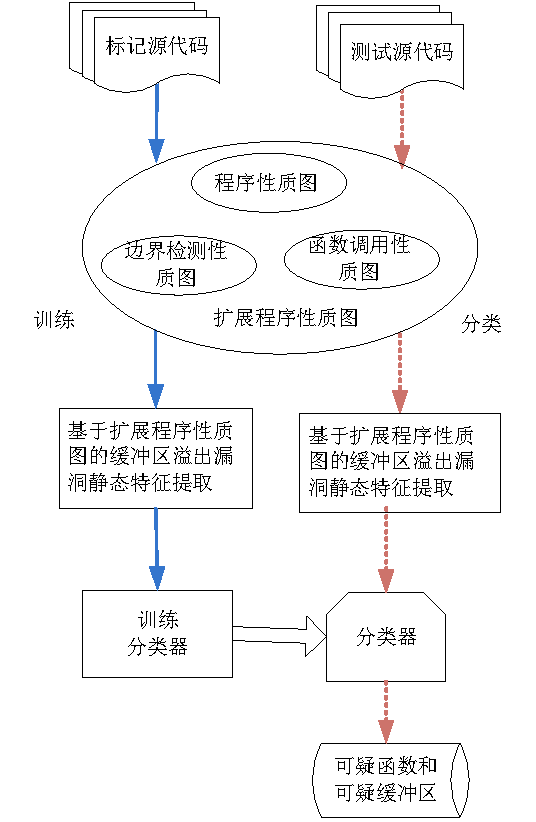
\includegraphics{基于机器学习的缓冲区溢出漏洞挖掘框架}
\caption{基于机器学习的缓冲区溢出漏洞挖掘框架}
\label{fig:基于机器学习的缓冲区溢出漏洞挖掘框架}
\end{figure}

\subsection{程序静态属性与映射规则}

通过分析和总结Kratkiewicz\upcite{kratkiewicz_evaluating_2005}提出的缓冲区溢出漏洞22种分类方法,本小节将缓冲区溢出漏洞的静态属性分为7类,分别为sink类型、缓冲区位置、索引/地址/长度复杂度、边界检测、循环/条件/函数调用深度以及是否输入可控。后续内容详细介绍了各类程序静态属性以及将程序静态属性映射到数字向量空间的规则。

\subsubsection{sink类型}

缓冲区溢出漏洞包含三种sink类型:指针解引用(Pointer Dereference)、数组写(Array Write)以及危险函数(Dangerous Function),如表\ref{Description_of_Three_Sink_Types}所示。如果函数中的一条语句符合三种sink类型的任意一条而又没有进行缓冲区边界检测,则程序就有可能发生缓冲区溢出。在C/C++中,数组的元素即可以通过指针解引用也可以用数组下标访问,但是对同一个缓冲区变量进行访问时很少混合使用,所以这里将二者分成两种类型。例如图\ref{CVE-2016-9537示例代码}中的第24、25行的变量src和dst就属于指针解引用这一类。危险函数是指像memcpy,strncpy等内存函数拷贝、字符串拼接函数,或者用户定义的具有相似功能的函数,例如程序图\ref{CVE-2016-9537示例代码}中第15、16、17行中的用户定义函数“\_TIFFmemcpy”,此函数和标准库函数memcpy的作用相同。如果一个用户定义的函数和标准库函数的参数个数相同、功能相近,则亦将此函数归为危险函数一类。
%另外某些格式化字符串函数也可能引起缓冲区溢出漏洞,但在本节中不予考虑。

\begin{table}[ht]
\begin{center}
\caption{缓冲区溢出漏洞三种sink类型} \label{Description_of_Three_Sink_Types}
\begin{small}
\begin{tabular}{lll}
\hline
{\bf Sink Type} & {\bf Example} & {\bf Mapping Value} \\
\hline
pointer dereference & *p++ = 1 &  1\\
\hline
array write & p[i] = 1 & 2 \\ \hline
dangerous function & strcpy(dst, src), strncpy(dst, src, n)\\
& strcat(dst, src), strncat(dst, src, n) & 3\\
& memcpy(dst, src, n), memmove(dst, src, n) &\\
& gets(str), fgets(str, n, fp)
 &  \\ \hline
\end{tabular}
\end{small}
\end{center}
\end{table}

\begin{figure}[h]
\begin{lstlisting}[language=C]
static int reverseSamplesBytes (uint16 spp, uint16 bps, uint32 width, uint8 *src, uint8 *dst)
  {
   int i;
   uint32  col, bytes_per_pixel, col_offset;
   uint8   bytebuff1;
   unsigned char swapbuff[32];
   if ((src == NULL) || (dst == NULL)){
     TIFFError("reverseSamplesBytes","Invalid input or output buffer");
     return (1);
  }
   bytes_per_pixel  = ((bps * spp) + 7) / 8;
   switch (bps / 8){...
     case 2: for (col = 0; col < (width / 2); col++){
       col_offset = col * bytes_per_pixel;                     
       _TIFFmemcpy (swapbuff, src + col_offset, bytes_per_pixel);
       _TIFFmemcpy (src + col_offset, dst - col_offset - bytes_per_pixel, bytes_per_pixel);
       _TIFFmemcpy (dst - col_offset - bytes_per_pixel, swapbuff, bytes_per_pixel);
     }
    break;
    case 1: /* Use byte copy only for single byte per sample data */
      for (col = 0; col < (width / 2); col++){ 
        for (i = 0; i < spp; i++){
          bytebuff1 = *src;
          *src++ = *(dst - spp + i);
          *(dst - spp + i) = bytebuff1;
        }
        dst -= spp;
      }
 ...}
\end{lstlisting}

\caption{CVE-2016-9537示例代码}
\label{CVE-2016-9537示例代码}
\end{figure}

\subsubsection{缓冲区位置}

缓冲区位置属性(Memory Location)描述的是缓冲区内存分布的位置,即栈、堆、数据段、BSS段与共享内存五种位置。从编程角度上,这五种内存位置的初始化方式是不相同的。局部非静态变量定义在栈上,通过malloc函数动态分配的缓冲区在堆上,数据段上存储的是全局初始化变量,BSS段上存储的是未初始化的全局或者静态变量,共享内存是特别分配的映射进或者映射出程序地址空间,并且通过特殊的操作系统函数(如Linux中的shmget,shmat,shmdt和shmctl)释放的内存区域。本节只考虑栈、堆和数据段三类缓冲区位置。三种内存位置被映射成一个三维向量表示为{(stack,heap,data segment)},提取静态属性时,根据缓冲区的初始化方式进行判断,如果相应的内存位置出现则将其赋为1,否则赋为0。例如图\ref{CVE-2016-9537示例代码}中的指针变量swapbuff,因为被声明为局部变量,所以对应的变量表示为$(1,0,0)$。

\subsubsection{容器}

容器属性(Container)描述的是缓冲区是否包含或者包含在一个什么样的容器当中。一般的,容器结构越复杂缓冲区的使用越容易出现错误。根据Zitser\upcite{zitser_testing_2004}统计,7\%的漏洞缓冲区包含在Union结构中,而在本节的训练集中,近30\%的漏洞包含在不同的容器中,所以这里将容器也作为一个属性,容器属性的示例和映射规则规则如表\ref{Container_Attributes}所示。这里将union和struct二者都映射成2,是因为他们在编程上的相似性,others表示更复杂的结构如多重union或者struct等。


\begin{table}[ht]
\begin{center}
\caption{容器属性} \label{Container_Attributes}
\begin{small}
\begin{tabular}{lll}
\hline
{\bf Instance } & {\bf Container Type} & {\bf Mapping Value} \\
\hline
p[256] & none &  0\\
\hline
p[256][256] & array & 1 \\ \hline
struct.p[256] & struct & 2  \\ 
union.p[256] & union & \\ \hline
ohters & others & 3 \\ \hline
\end{tabular}
\end{small}
\end{center}
\end{table}

\subsubsection{索引/地址/长度复杂度}

索引复杂度属性描述的是数组索引的复杂度,其引入是基于这样一个假设:对于索引值的操作越复杂,数组越容易发生溢出。索引复杂度可以分成六种:常量(constant)、加减法(addition)、乘除法(multiplication)、非线性(non-linear)、函数调用(function call)以及数组访问(array access),如表\ref{Index_Type}所示。加减法操作包括类似加法和减法的操作,自增和自减操作也归入此类。乘除法操作包含乘法、除法以及逐位左移和右移等操作。非线性操作包含取模以及标准库的其他非线性函数例如pow()与sqrt()等。函数调用操作描述的是数组索引操作是否包含函数的返回值(除标准库的非线性函数)。数组访问操作表示数组索引操作是否包含数组访问。尽管很难被利用,常量索引还是有造成缓冲区溢出,所以也被列为索引操作之一。除了常量类型,其他的索引操作类型都有两种不同的呈现方式:p[i-8]和(p-8)[i]。

图\ref{accumulating_the_operations_of_i}是获取复杂度的一个简单的示例。i是数组p的索引变量,沿着数据流获取对i的操作形成一个六维向量{(0,1,0,0,1,1)}。

\begin{table}[ht]
\begin{center}
\caption{索引操作类型} \label{Index_Type}
\begin{small}
\begin{tabular}{lll}
\hline
{\bf Operation Type } & {\bf Instance}\\
\hline
constant & p[256] \\ \hline
addition & p[i+8], p[i-8], (p+8)[i], (p-8)[i] \\ \hline
multiplication & p[i*8], p[i/8], p[i$\gg$8], p[i$\ll$8], (buf+8*n)[i] \\ \hline
non-linear & p[i\%8], p[pow(i, j)], p[sqrt(i)] \\ \hline
function call & p[f(i)], (p+f(n))[i], (getAdtres(n))[i] \\ \hline
array access & p[buf[i]], (p+buf[n])[i], (buf[n])[i] \\ \hline
\end{tabular}
\end{small}
\end{center}
\end{table}

\begin{figure}[htp]
\centering
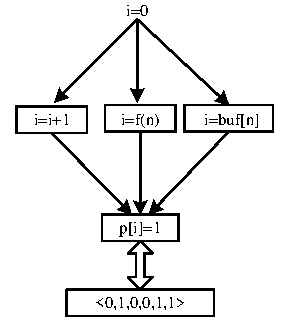
\includegraphics{accumulating_the_operations_of_i}
\caption{变量i复杂度的获取}
\label{accumulating_the_operations_of_i}
\end{figure}

地址/长度复杂度属性与索引复杂度相似,其示例和映射规则如表\ref{ADDRESS_TYPE}和表\ref{LENGTH_TYPE}所示。地址和长度复杂度也被映射成一个六维向量,相应的操作每出现一次对应的值就加1。对于图\ref{CVE-2016-9537示例代码}第24行、25行的缓冲区变量src和dst,地址复杂度属性对应的向量为{(0,1,0,0,0,0)}和{(0,3,0,0,0,0)}。对于危险函数sink类型的缓冲区变量swapbuff,其长度复杂度向量为{(0,1,2,0,0,0)}。另外,索引/地址/长度复杂度属性都需要将缓冲区别名考虑在内,即对缓冲区别名的操作需要类累加到相应的向量中。

\begin{table}[ht]
\begin{center}
\caption{地址操作类型} \label{ADDRESS_TYPE}
\begin{small}
\begin{tabular}{lll}
\hline
{\bf Operation Type } & {\bf Instance}\\
\hline
constant & not appliable \\ \hline
addition & *p(i+8), *p(i-8) \\ \hline
multiplication & *(p+i*8), *p(i/8), *p(i$>>$8), *p(i$<<8$) \\ \hline
non-linear & *(p+i\%8), (p+pow(i, j)), *(p+sqrt(i)) \\ \hline
function call & *(p+f(i)), *(getAddress()) \\ \hline
array access & *(p+buf[i]) \\ \hline
\end{tabular}
\end{small}
\end{center}
\end{table}


\begin{table}[ht]
\begin{center}
\caption{长度操作类型} \label{LENGTH_TYPE}
\begin{small}
\begin{tabular}{lll}
\hline
{\bf Operation Type } & {\bf Instance}\\ \hline
constant & memcpy (dest, src, 256) \\ \hline
addition & memcpy (dest, src, i+256) \\ \hline
multiplication & memcpy (dest, src, i*8) \\ \hline
non-linear & memcpy (dest, src, i\%8) \\ \hline
function call & memcpy (dest, src, f(n)) \\ \hline
array access & memcpy (dest, src, buf[255]) \\ \hline
\end{tabular}
\end{small}
\end{center}
\end{table}

\subsubsection{边界检测}

虽然静态分析不能精确的捕捉缓冲区的边界检测(Sanitization)信息,但依然可以通过边界检测的模式去近似的估计。如果一条语句符合以下的几种模式,就可以近似的认为编程人员已经考虑了边界检测,这些模式出现的次数越多则说明编程人员添加边界检测的概率要更高。边界检测可以分为以下三种类型。

\begin{enumerate}[1]
\item 直接边界检测:假设$P=<n_1, n_2,...,n_N>$是CFG上的一条路径,$0<i<N$。如果$n_j$是一个sink节点,$n_i$是一个条件语句节点,若程序满足以下任一条件,则$n_i$是一个直接边界检测节点。(1)$n_j$是一个数组写sink,$iv$是$n_j$的数组索引变量或表达式,如果$n_i$使用$iv$;(2)$n_j$是一个危险函数sink,$l$是$n_j$索要拷贝的长度变量或者表达式,如果$n_i$使用$l$;(3)$buf$是$n_j$的缓冲区变量且$n_i$使用了$buf$。像$n_i$这样的节点在函数中每出现一次,直接边界检测的值加1。图\ref{CVE-2016-9537补丁程序}第1行的条件语句就是一个直接边界检测。
\item 间接边界检测:此类边界检测只适用于数组写sink和危险函数sink;假设$s$是一个语句节点,$Use(s)=\{v|\text{s是一个定义语句且使用v}\}$,$DDUse(v)$表示所有$v$数据依赖的变量,即$DDUse(v) = \bigcup_{v_c \in Use(v)} v_c \cup DDUse(v_c)$;对于图\ref{CVE-2016-9537示例代码}第15行的长度变量{bytes\_per\_pixel},$DDUse(bytes_per_pixel) = {bps, spp}$;假设$P=<n_1, n_2,...,n_N>$是CFG上的一条路径,$0<i<N$。如果$n_j$是一个sink节点,$n_i$是一个条件语句节点,$iv$是一个长度变量或者数组索引变量,$n_i$使用$v$且$v \in DDUse(iv)$,在$n_i$是一个间接边界检测节点。例如图\ref{间接边界检测示例程序}的第1行就是一个间接边界检测节点。
\item 过程间检测:如果函数的参数与长度变量、数组索引或者缓冲区变量有数据依赖关系,且参数出现在上级调用函数的条件语句中,则称此条件语句是一个过程间边界检测;图\ref{过程间边界检测示例程序}是一个过程间边界检测的示例。
\end{enumerate}

此外,一些条件语句虽然符合上面的描述,但不能算作为边界检测。例如第7行的条件语句不能被当做直接边界检测,因为将一个缓冲区变量和NULL做比较的作用是判断一个指针是否为NULL。边界检测属性被映射成一个三维向量,每一类边界检测出现一次则相应的数值加1。

\begin{figure}[h]
\begin{lstlisting}[language=C]
if( bytes_per_pixel > sizeof(swapbuff) ){
  TIFFError("reverseSamplesBytes","bytes_per_pixel too large");
  return (1);
}

\end{lstlisting}

\caption{CVE-2016-9537补丁程序}
\label{CVE-2016-9537补丁程序}
\end{figure}


\begin{figure}[h]
\begin{lstlisting}[language=C]
if(i<256)
{
  buf[i+j] = 1;
}
\end{lstlisting}

\caption{间接边界检测示例程序}
\label{间接边界检测示例程序}
\end{figure}


\begin{figure}[h]
\begin{lstlisting}[language=C,caption=过程间边界检测示例程序,label=过程间边界检测示例程序]
void woo(int arg){
  if(arg<256)
  {
    foo(arg) ;
  }
}
void foo(int param)
{
  buf[param]=1;
}
\end{lstlisting}

\caption{过程间边界检测示例程序}
\label{过程间边界检测示例程序}
\end{figure}



\subsubsection{循环/条件/函数调用深度}

循环/条件/函数调用深度属性反映了程序的复杂度。其中,循环/条件深度表示包裹sink语句循环/条件层次,函数调用深度描述从入口函数到sink函数之间的函数调用数量,函数调用深度可以通过\ref{扩展的程序性质图}引入的函数调用性质图获取。循环/条件/函数调用深度属性被映射成一个三维向量。对于图\ref{CVE-2016-9537示例代码}的sink变量src,其调用链为$main \rightarrow createCroppedImage \rightarrow mirrorImage \rightarrow reverseSanplesBytes$,switch语句在本节中也被当做条件语句,所以其向量为(2,1,4)。

\subsubsection{输入可控}

输入可控用于判断sink语句是否和输入有数据依赖关系,此属性的判定和\ref{缓冲区溢出漏洞检测}节相同。输入数据可以是函数的参数,也可以通过命令行、环境变量、文件输入或者网络传入的变量。如果sink语句输入可控,则将其设为1,否则设为0。

综上,将七类属性映射的向量串接得到一个18维向量,此向量将被用来训练分类器。

\subsection{扩展的程序性质图}
\label{扩展的程序性质图}

\ref{程序性质图}节中介绍了由过程内的抽象语法树、控制流图以及数据依赖图融合而成的程序性质图。在程序性质图中,每个节点都拥有多个属性,节点之间通过各类边连接,每条边亦拥有多个属性。通过抽象语法树性质图可以获取源代码的所有操作数和操作符,所以sink类型和容器属性可以很容易的获取;获取缓冲区位置和输入可控属性需要抽象语法树和数据依赖图;条件/循环深度需要抽象语法树和控制流图;直接/间接边界检测以及索引/地址/长度复杂度需要三类性质图的结合。但是,程序性质图不能处理过程间边界检测和函数调用深度,因为二者的获取需要过程间的数据依赖和控制依赖关系。为了解决这个问题,将过程间边界检测性质图和函数调用性质图并入到程序性质图形成扩展的程序性质图。

\begin{definition}
 \label{过程间边界检测程序性质图}
 过程间边界检测性质图$G=(V_A,E_{IP},\lambda_{IP} ,\mu_IP, s, d)$,$V_{A}$是抽象语法树节点,$E_{IP}$连接条件语句节点和被调用函数的sink语句节点,$\lambda_{IP}$,$\lambda_{IP}:E_{IP} \rightarrow \sum_{IP}$,其中$\sum_{IP}=\{IC, ID\}$, $IC$表示过程间控制依赖,$ID$表示过程间数据依赖,过程间数据依赖边被赋予一个$symbol$属性。
\end{definition}

图\ref{过程间边界检测和函数调用性质图解释程序}为过程间边界检测和函数调用性质图解释程序。图\ref{简化程序性质图}为其简化的程序性质图(删除了部分抽象语法树节点和边),图\ref{过程间边界检测性质图和函数调用性质图}(a)是的过程间边界检测性质图示意图。通过对比图\ref{简化程序性质图}和图\ref{过程间边界检测性质图和函数调用性质图},可以看出为了产生$E_{IP}$,条件语句if(size<100)必须和函数具有数据和控制依赖关系且memcpy函数的参数src,count必须和foo函数的参数有数据依赖关系。

\begin{definition}
 \label{函数调用性质图}
 过程间边界检测性质图$G=(V_{A},E_{CC},\lambda_{CC} ,\mu_CC, s, d)$,$V_{A}$是抽象语法树节点,如果函数$f_1$调用$f_2$,则$E_{IP}$连接两个函数定义节点,$\lambda_{IP}:E_{CC} \rightarrow \sum_{CC}$,其中$\sum_{IP}=\{CC\}$,每条边被赋予一个$symbol$属性,用于表示函数之间传递的符号。
\end{definition}

图\ref{过程间边界检测性质图和函数调用性质图}(b)图 \ref{过程间边界检测和函数调用性质图解释程序}的函数调用性质图示意图。函数调用性质图能获取函数调用深度,而且能获取影响sink语句的输入源。

\begin{figure}[h]
\begin{lstlisting}[language=C]
int main(int argc, char **argv){
    int i = atoi(argv[1]);
    char *p = argv[2];
    woo(p, i);
}
void woo(char* src, int size){
    if(n<100){
        foo(src, size);
    }
}
void foo(char* src, int n){
    char dst[200];
    int count = n+100;
    memcpy(dst, src, count);
}
\end{lstlisting}

\caption{过程间边界检测和函数调用性质图解释程序}
\label{过程间边界检测和函数调用性质图解释程序}
\end{figure}

\begin{figure}[htp]
\centering
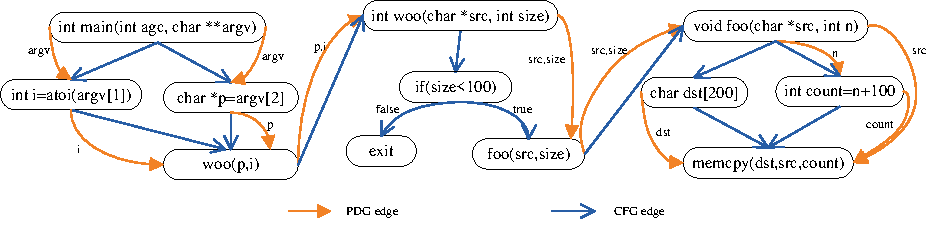
\includegraphics{Simplified_CPG_of_code_for_Fig7}
\caption{图\ref{过程间边界检测和函数调用性质图解释程序}的简化程序性质图}
\label{简化程序性质图}
\end{figure}

\begin{figure}[htp]
\centering
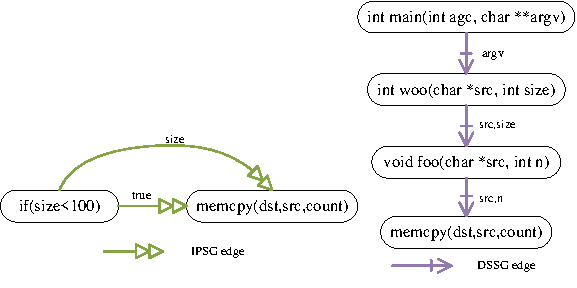
\includegraphics{IPSG_and_DSSG}
\caption{图\ref{过程间边界检测和函数调用性质图解释程序}过程间边界检测性质图和函数调用性质图}
\label{过程间边界检测性质图和函数调用性质图}
\end{figure}

将过程间边界检测性质图,函数调用性质图并入程序性质图形成扩展的程序性质图$G=(V,E,\lambda, \mu, s, d)$,其中,
\begin{align*}
& V = V_{A} \\
& E = E_{A} \cup E_{C} \cup E_{P} \cup E_{IP} \cup E_{CC}\\
& \lambda = \lambda_{A} \cup \lambda_{C} \cup \lambda_{P} \cup \lambda_{IP} \cup \lambda_{CC} \\
& \mu = \mu_{A} \cup \mu_{C} \cup \mu_{P} \cup \mu_{IP} \cup \mu_{CC}
\end{align*}
通过组合程序性质图的基本遍历方式,获取缓冲区溢出漏洞静态属性。

\subsection{实验与分析}

\subsubsection{实验设计}

(1)实验目的与评估参数

通过实验以及和其他工具对比,验证基于机器学习的缓冲区溢出漏洞方法的有效性。方法的性能通过混淆矩阵\upcite{stehman_selecting_1997}展示,如表\ref{confusion_matrix}所示。混淆矩阵描述了实际类别和挖掘类别的交叉组合,即真正类(True Positive,TP),假负类(False Positive,FP),真负类(True Negative,TN)以及假负类(False Negative,FN)。在漏洞挖掘领域,FP又被称为误报,表示一个非漏洞被分类器归为漏洞;FN又称为漏报,表示一个漏洞被分类器归为非漏洞;TP表示一个漏洞被分类器归为漏洞;TN表示一个非漏洞被分类器归为漏洞。在一个正常的程序中,非漏洞函数要远比漏洞函数多,如此会造成训练和测试集的不均衡,所以再次添加了其他的衍生评估参数,即召回率(recall)同时也被称为真值率(True Positive Rate,TPR),真负率(True Negative Rate,TNR),精度(precision)也被称为阳性预测值(Positive Predictive Value,PPV)以及$F_1$值,此四参数的计算如式\ref{衍生标准}所示。

\begin{table}[ht]
\begin{center}
\caption{混淆矩阵} \label{confusion_matrix}
\begin{small}
\begin{tabular}{lll}
\hline
 & {\bf Predicted Positive} & {\bf Actual Positive}\\ \hline
{\bf Actual Positive} & True positive (TP) & False Negative (FN)\\ \hline
{\bf Actual Negative} & False Positive(FP) & True Negative (TN)\\ \hline
\end{tabular}
\end{small}
\end{center}
\end{table}

\begin{equation}
\begin{split}
\label{衍生标准}
& recall = TP/(TP+FN) \\
& TNR = TN/(FP+TN) \\
& precision = TP/(TP+FP) \\
& F_1 = 2 \times (recall \times precision)/(recall + precision)
\end{split}
\end{equation}

(2)实验环境与过程

本方法选取了8个开源软件作为训练集,分别为ffmpeg,HDF5,libtff,mupdf,openssl,qemu,zziplib以及blueZ,如表\ref{CVE_List_For_Attribute_Extraction}所示。从这些软件中,结合CVE漏洞库手动审计了58个缓冲区溢出漏洞函数以及另外的174个非漏洞函数,对于所有的函数,都选择一个缓冲区代表函数提取静态属性。列Vul-Num和Not-Vul-Num分别表示漏洞函数和非漏洞函数数量。漏洞函数被标记为1,非漏洞函数被标记为0。

\begin{table}[ht]
\begin{center}
\caption{实验数据列表} \label{CVE_List_For_Attribute_Extraction}
\begin{small}
\begin{tabular}{llll}
\hline
{\bf Program } & {\bf CVE-ID} & {\bf Vul-Num} & {\bf Not-Vul-Num}\\ \hline
ffmpeg & CVE-2016-7562, CVE-2016-6920, \\ &CVE-2016-10192, CVE-2016-10191,\\ & CVE-2016-10190, CVE-2016-8364,\\ & CVE-2014-5271, CVE-2014-3157,\\ & CVE-2014-2263, CVE-2013-0894,\\ & CVE-2013-0868, CVE-2013-0863,\\ & CVE-2012-0947, CVE-2012-0857,\\ & CVE-2012-0856, CVE-2012-0855,\\ & CVE-2012-0848, CVE-2012-0847 & 18 & 54\\ \hline

HDF5 & CVE-2016-4333, CVE-2016-4330 & 2 & 6 \\ \hline

libtiff & CVE-2017-5225, CVE-2016-9540, \\ & CVE-2016-9537, CVE-2016-9536, \\ & CVE-2016-9535, CVE-2016-9533, \\ & CVE-2016-5652, CVE-2016-5319, \\ & CVE-2016-5318, CVE-2016-5102, \\ & CVE-2016-3991, CVE-2016-3990, \\ & CVE-2016-3632, CVE-2016-3624, \\ & CVE-2015-8784, CVE-2015-8782, \\ & CVE-2013-4244, CVE-2013-4231 & 18 & 54 \\ \hline

mupdf & CVE-2017-5869, CVE-2016-6525, \\ & CVE-2014-2013, CVE-2011-0341 & 4 & 12\\ \hline

openssl & CVE-2016-2182, CVE-2015-0235,\\ & CVE-2014-3512 & 3 & 9\\ \hline

qemu & CVE-2016-7170, CVE-2016-5238,\\ & CVE-2016-4439, CVE-2013-4151,\\ &  CVE-2013-4150 
 & 5 & 15\\ \hline
 
zziplib & CVE-2017-5976, CVE-2017-5975,\\ & CVE-2017-5974, CVE-2017-1614 & 4 & 12\\ \hline

BlueZ & CVE-2016-9917, CVE-2016-9804,\\ & CVE-2016-9803,  CVE-2016-9800 & 4 & 12\\ \hline
\end{tabular}
\end{small}
\end{center}
\end{table}

哪种分类器的性能更好是不可预知的,所以需要测试不同的分类器算法性能。本实验利用了五个著名的分类器:K近邻法(K-Nearest Neighbors,KNN),决策树(Decision Tree,DT),朴素贝叶斯(Naive Bayes,NB),AdaBoost以及支持向量机(Support Vector Machines,SVM)。为了这是的评估分类器性能,本实验采用了10重交叉验证。各分类器参数设定如下:KNN中的参数k为7,DT算法用的是C4.5,AdaBoost使用的弱分类器的数量是20,SVM使用的是RBF核,参数C=10,$\gamma = 0.01$。实验的采用的硬件环境是Inter Xeon CPU E3-1231 v3 @ 3.40GHz,16G RAM。

实验过程如图\ref{fig:基于机器学习的缓冲区溢出漏洞挖掘框架}所示。首先,利用训练集,根据缓冲区溢出漏洞的静态特征训练出分类器;然后,从新的源代码中抽取缓冲区溢出漏洞静态特征并向量化,利用分类器挖掘缓冲区溢出漏洞。

\subsubsection{结果分析}

五个分类器的性能展示如表\ref{PERFORMANCES_OF_OUR_FIVE_CLASSIFIER_ALGORITHMS}所示。平均recall为83.5\%,即58个漏洞平均可以检测出48个。平均TNR是87.3\%,即174个非漏洞152个检测正确。平均precision为68.9\%,平均$F_1$为75.2\%,两个指数不高的原因是训练集是不均衡的,非漏洞是漏洞的3倍。在漏洞检测领域,尽可能的检测最多的漏洞比减少误报更为重要,所以可以认为NB是5个分类器当中表现最好,将96.6\%的漏洞分类正确。

\begin{table}[ht]
\begin{center}
\caption{五个分类器的性能} \label{PERFORMANCES_OF_OUR_FIVE_CLASSIFIER_ALGORITHMS}
\begin{small}
\begin{tabular}{lllllllll}
\hline
 {\bf Classifierss}& {\bf TP} & {\bf FN} & {\bf FP} & {\bf TN} & {\bf recall(\%)} & {\bf TNR(\%)} & {\bf precision(\%)} & {\bf $F_1$(\%)}\\ \hline
KNN & 42 & 16 & 20 & 154 & 72.4 & 88.5 & 67.7 & 70\\ \hline
DT & 44 & 14 & 31 & 143 & 75.9 & 82.2 & 58.7 & 66.2\\ \hline
NB & 56 & 2 & 27 & 147 & 96.6 & 84.5 & 67.5 & 79.5\\ \hline
Adaboosting & 46 & 12 & 15 & 159 & 79.3 & 91.4 & 75.4 & 77.3\\ \hline
SVM & 54 & 4 & 18 & 156 & 93.1 & 89.7 & 75 & 83.1\\ \hline
\end{tabular}
\end{small}
\end{center}
\end{table}

表\ref{PERFORMANCE_OF_BOMINER_FOR_OUR_TEST_SUITE}所示是本章方法和BOMiner\upcite{padmanabhuni_predicting_2014}的对比。
%Padmanabhuni在\upcite{padmanabhuni_predicting_2014}中设计了一个利用机器学习算法挖掘缓冲区溢出漏洞的工具BOMiner。
BOMiner最多能检测出38个漏洞,比本章方法最差的分类器KNN少4个,比最优的分类器NB少18个。BOMiner最高的recall是65.5\%,比本章训练的所有分类器低。图\ref{compareToBOMiner}(a)是本章方法和BOMiner在混淆矩阵平均值上的比较。本章方法平均比BOMiner多发现14.8个漏洞,10.4个非漏洞。图\ref{compareToBOMiner}(b)是本章方法和BOMiner在衍生评估参数平均值上的比较。相比与BOMiner,本章方法在recall上增加了17.5\%,$F_1$值增加了21.1\%。造成性能差距的主要原因是BOMiner并没有更深入的讨论数组写sink和危险函数sink,BOMiner在处理这两类sink时获取的信息太少以至于不能正确的分类漏洞和非漏洞。

\begin{table}[ht]
\begin{center}
\caption{BOMiner性能} \label{PERFORMANCE_OF_BOMINER_FOR_OUR_TEST_SUITE}
\begin{small}
\begin{tabular}{lllllllll}
\hline
 {\bf Classifierss}& {\bf TP} & {\bf FN} & {\bf FP} & {\bf TN} & {\bf TPR(\%)} & {\bf TNR(\%)} & {\bf precision(\%)} & {\bf $F_1$(\%)}\\ \hline
KNN & 29 & 29 & 21 & 153 & 50.0 & 87.9 & 58 & 53.7\\ \hline
DT & 31 & 27 & 35 & 139 & 53.4 & 79.9 & 47 & 50\\ \hline
NB & 38 & 20 & 46 & 128 & 65.5 & 73.6 & 45.2 & 53.5\\ \hline
Adaboosting & 33 & 25 & 28 & 146 & 56.9 & 83.9 & 54.1 & 55.5\\ \hline
SVM & 37 & 21 & 33 & 141 & 63.8 & 81 & 52.9 & 57.8\\ \hline
\end{tabular}
\end{small}
\end{center}
\end{table}

\begin{figure}[htb]
\begin{center}
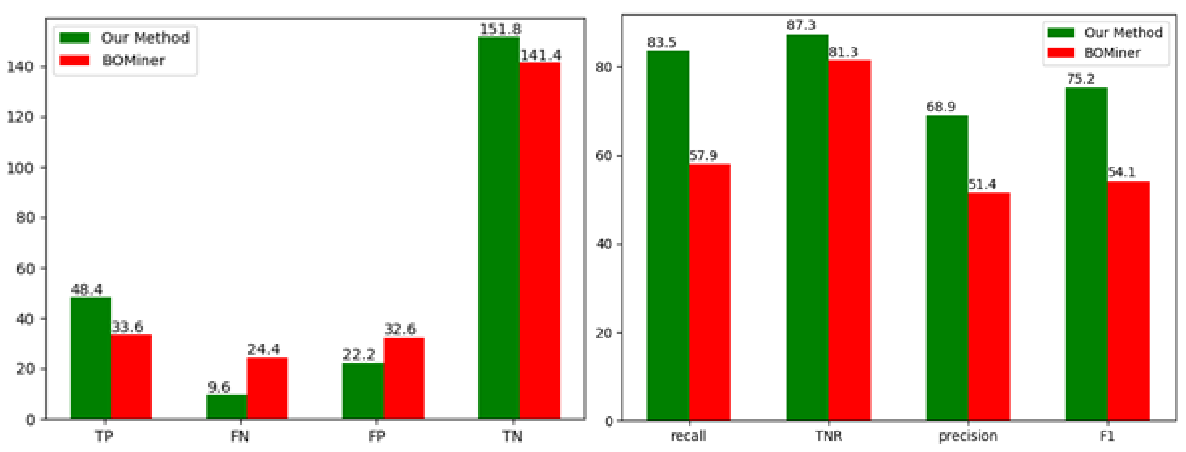
\includegraphics[width=10cm]{compareToBOMiner}
\end{center}
\caption{(a) 和BOMiner在混淆矩阵平均值的比较, (b) 和BOMiner在衍生评估参数上的比较}
\label{compareToBOMiner}
\end{figure}

表\ref{和Joern的混淆矩阵比较}是本章方法和Joern\upcite{yamaguchi_modeling_2014}的性能比较。Joern能够以很低的误报检测源代码缓冲区溢出漏洞。通过设计特定的搜索模式,Joern从linux内核中的驱动中检测了6个缓冲区溢出漏洞。但是,通过研究CVE数据库发驱动中已发现的漏洞有18个,通过分析驱动源代码发现有179个非漏洞sink函数。使用本章方法,最少可以检测12个缓冲区漏洞,五个分类器当中最小的recall是66.7\%,在这两个参数上本章方法要比Joern表现好。最高的TNR是93.8\%,比Joern低6\%。图\ref{compareToJoern}(a)是本章方法在linux驱动上和Joern的比较,本章方法平均比Joern多8.2个漏洞,平均比Joern多11.8个误报。图\ref{compareToJoern}(b)是本章方法衍生参数和Joern的比较,本章方法的平均recall是78.9\%,比Joern高了45.6\%,在TNR上仅仅低了6\%;平均precision比Joern低了24.1\%;平均$F_1$值比Joern高15.5\%。造成性能差异的原因有两个:(1)Joern仅仅专注于memcpy引起的缓冲区漏洞;(2)Joern使用的两个边界检测规则,即目的缓冲区的动态分配和关系表达式都可以当做本章的直接边界检测属性,二者虽然可以减少误报但增加了误报。

\begin{table}[ht]
\begin{center}
\caption{与Joern性能比较} \label{和Joern的混淆矩阵比较}
\begin{small}
\begin{tabular}{lllllllll}
\hline
 {\bf Classifierss}& {\bf TP} & {\bf FN} & {\bf FP} & {\bf TN} & {\bf TPR(\%)} & {\bf TNR(\%)} & {\bf precision(\%)} & {\bf $F_1$(\%)}\\ \hline
Joern & 6 & 12 & 2 & 177 & 33.3 & 98.9 & 75 & 46.2\\ \hline
KNN & 12 & 6 & 11 & 168 & 66.7 & 93.9 & 52.2 & 58.6\\ \hline
DT & 14 & 4 & 14 & 165 & 77.8 & 92.2 & 50 & 60.9\\ \hline
NB & 15 & 3 & 15 & 164 & 83.3 & 91.6 & 50 & 62.5\\ \hline
Adaboosting & 14 & 4 & 12 & 167 & 77.8 & 93.3 & 53.8 & 63.6\\ \hline
SVM & 16 & 2 & 17 & 162 & 88.9 & 90.5 & 48.5 & 62.8\\ \hline
\end{tabular}
\end{small}
\end{center}
\end{table}

\begin{figure}[htb]
\begin{center}
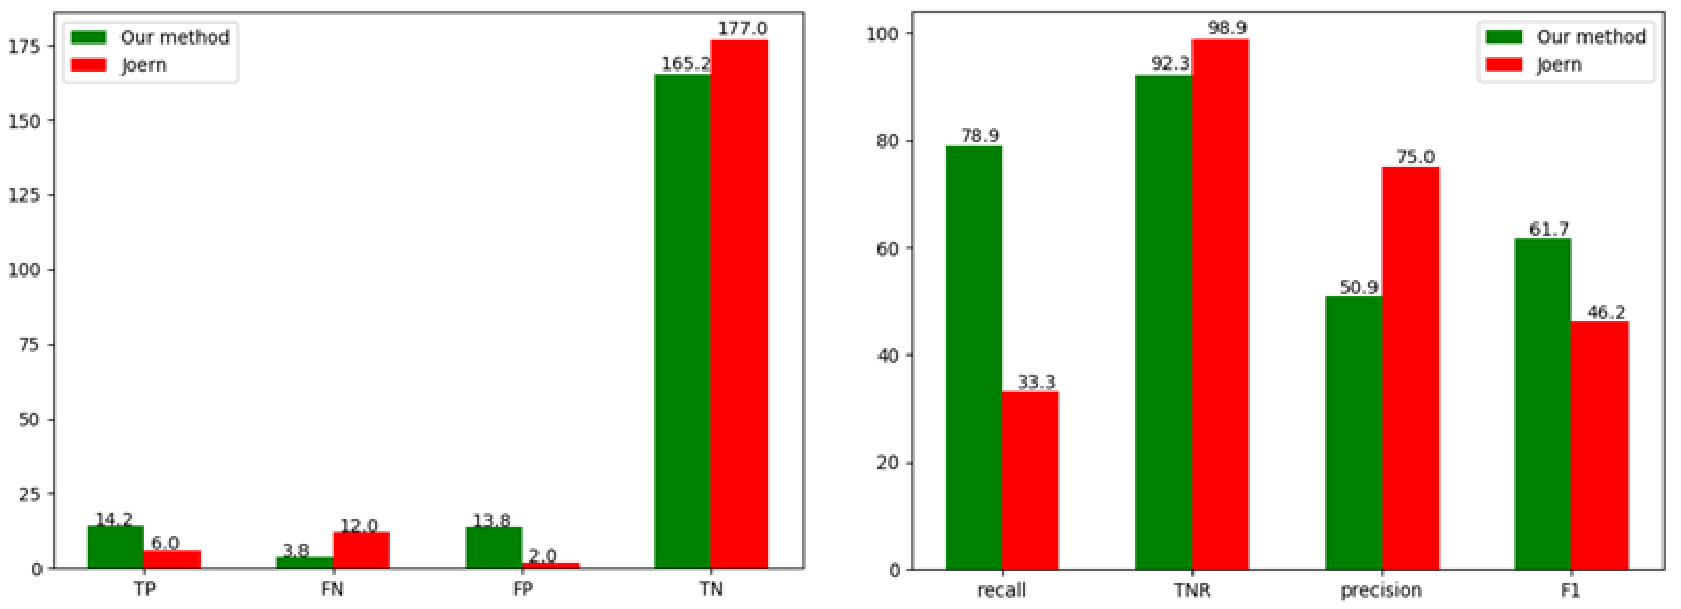
\includegraphics[width=10cm]{compareToJoern}
\end{center}
\caption{(a) 和Joern在混淆矩阵平均值的比较, (b) 和Joern在衍生评估参数上的比较}
\label{compareToJoern}
\end{figure}

除了在在训练集上检验方法的性能,本节在poppler 0.10.6进行了测试,并与FlawFinder做了比较,以验证本章方法在减少可以函数数量的作用。Poppler是一个广泛应用的开源PDF库,历史上被发现了很多漏洞。至今poppler 0.10.6已经被发现了10个被证实的CVE:CVE-2015-8868, CVE-2013-1788, CVE-2010-3704, CVE-2009-3938, CVE-2009-3608, CVE-2009-3607, CVE-2009-3606, CVE-2009-3604以及 CVE-2009-3603。表\ref{PERFORMANCES_OF_OUR_FIVE_CLASSIFIERS_ON_POPPLER0.10.6}展示了5个分类器在poppler 0.10.6的性能,SVFs(Suspect Vulnerable Functions)是TP和FP之和,表示需要考虑的可以函数;Sink (Sink Functions表)示所有的满足三种sink类型的函数;All (All Functions)表示poppler 0.10.6源码中包含的所有函数数量。5个分类器的平均TP为8.8,表示本方法可以检测11个漏洞中的9个。9个CVE有11个漏洞的原因是CVE-2013-1788有三个漏洞函数。平均recall是80\%,平均TNR为94\%,因为非漏洞函数的数量远小于漏洞函数数所以平均$F_1$较低只有28.9\%。从实验结果可以看出,本方法可以以很低的漏报率发现绝大多数漏洞。

Flawfinder\upcite{flawfinder_nodate}是一个基于语法分析的静态漏洞扫描器。当在poppler 0.10.6运行Flawfinder时,其能发现11个中的8个缓冲区溢出漏洞,稍稍低于本章方法。但是Flawfinder同时产生了500误报,是本章方法的12倍之多。以此可以看出,本章方法在缩小可疑函数上效果非常显著。

\begin{table}[ht]
\newcommand{\tabincell}[2]{\begin{tabular}{@{}#1@{}}#2\end{tabular}}
\begin{center}
\caption{五个分类器在Poppler0.10.6上的性能测试} \label{PERFORMANCES_OF_OUR_FIVE_CLASSIFIERS_ON_POPPLER0.10.6}
\begin{small}
\begin{tabular}{llllllllllll}	
\hline
 {\bf }& {\bf TP} & {\bf FN} & {\bf FP} & {\bf TN} & {\bf recall} & {\bf TNR} & {\bf precision} & {\bf $F_1$} & {\bf SVFs} & {\bf Sink} & {\bf All}\\ \hline
KNN & 7 & 4 & 37 & 648 & 63.6 & 94.6 & 15.9 & 25.4 & 44 & \multirowcell{5}{685} & \multirowcell{5}{4876}\\ \cline{1-10}
DT & 8 & 3 & 44 & 641 & 72.7 & 93.6 & 15.4 & 25.4 & 52  \\ \cline{1-10}
NB & 10 & 1 & 52 & 633 & 90.9 & 92.4 & 16.1 & 27.4 & 62  \\ \cline{1-10}
Ada & 9 & 2 & 39 & 646 & 81.8 & 94.3 & 18.8 & 30.6 & 48  \\ \cline{1-10}
SVM & 10 & 1 & 35 & 650 & 90.9 & 94.9 & 22.2 & 35.7 & 45  \\ \hline
\end{tabular}
\end{small}
\end{center}
\end{table}

\section{本章小结}

本章主要研究了基于程序性质图源代码漏洞挖掘方法与基于机器学习的缓冲区溢出漏洞挖掘方法,具体包括以下两个内容。

(1)提出了基于程序性质图的源代码漏洞挖掘方法,用于标定可疑区域。该方法首先利用鲁棒的中间表示生成语法分析树、抽象语法树、控制流图、数据流图;然后通过性质图将三种中间表示聚合成统一的程序性质图,并定义程序性质图遍历方式;最后根据缓冲区溢出漏洞、格式化字符串漏洞以及UAF漏洞的特征给出三类漏洞的挖掘算法。通过在poppler0.10.6、a2ps4.14以及libxml2-2.9.3三个软件上的实验表明,基于程序性质图能够有效的挖掘源代码漏洞。

(2)提出了一种基于机器学习的缓冲区溢出漏洞挖掘方法。该方法首先将22种程序静态特征约简成7类,分别是sink类型、缓冲区位置、容器、索引/地址/长度复杂度、边界检测、循环/条件/函数调用深度以及是否输入可控;其次通过扩展的程序性质图提取静态特征;然后在CVE库中查找现存的缓冲区溢出程序和未溢出程序作为训练集,并选取5种有监督机器学习算法在训练集中训练分类器;最后利用分类器在新的源代码程序中挖掘漏洞。实验结果表明,5个分类器的平均召回率(recall亦称为TPR,True Positive Rate) 是83.5\%,平均真负率(TNR,True Negative Rate)为85.9\%,最好的召回率达到了96.6\%,最好的真负率达到了91.4\%。因为实验的数据是非均衡数据,所以准确率(Precision)和$F_1$稍低,分别为68.9\%和75.2\%。将此方法应用到poppler0.10.6上,并和经典的静态分析工具FlawFinder做对比,本方法能够将误报率消减到1/12。实验证明,本方法能够有效的挖掘缓冲区溢出漏洞。

\chapter{基于细粒度变异的导向模糊测试技术研究}

模糊测试已被证明是一种非常强大的软件漏洞测试方法,是工业界和学术界研究的热点。但是模糊测试的变异具有随机性,从而导致测试不可控且很难测试特定目标。
%在安全性重要性比较高的软件中,模糊测试发现了绝大多数远程程序执行漏洞和权限提升漏洞。
%但是模糊测试一样有它的局限性,盲目的随机的变异测试用例很难到达测试程序的特定路径,导致一些漏洞很难被触发。
在源代码软件的漏洞挖掘中,一些可疑的漏洞触发点可以通过静态分析获取。所以,如何动态的产生测试用例到达可疑漏洞触发点是一项重要的研究内容。现有的主要的导向测试研究都是基于符号执行的\upcite{sparks_automated_2007, santelices_test-suite_2008, person_directed_2011, marinescu_katch:_2013, ma_directed_2011, haller_dowsing_2013, christakis_guiding_2016, bohme_regression_2013},又可称为导向白盒模糊测试。但是导向符号执行在程序分析和约束求解上耗费了大量的时间。在每一轮的测试中,为了到达目标区域,动态符号执行需要利用程序判断哪些分支需要反转,并沿着路径收集约束信息,最后调用约束求解器生成新的测试用例。而模糊测试不需要进行约束求解,仅仅通过变异生成测试用例。在相同的时间内,模糊测试产生的测试用例要比动态符号执行高几个数量级。此外,符号执行还有其他的问题如环境交互问题和循环问题\upcite{baldoni_survey_2016}。Macel Bohme\upcite{bohme_directed_2017}提出了一种基于AFL(American fuzzy lop)\upcite{noauthor_american_nodate}的导向模糊测试工具AFL-go。此方法设计了一种用于衡量测试用例到目标区域的距离测度以及一种能量分配策略;随着测试时间的增加,AFL-go通过增加距离近的测试用例的变异次数,减少距离远的测试用例的变异次数,从而完成目标区域导向。但是AFL-go的变异还是具有很大的盲目性。
%不能规划测试用例的变异方向的缺点。
%从而导致导向效率不高。

本章提出了一种细粒度变异的导向模糊测试方法。该方法首先使用AFL-go收集测试用例;然后利用时间递归神经网络(Long Short-Term Memory,LSTM)训练出一个模型,用于判断哪些字段对靠近目标区域其关键作用,同时收集每个字段的权重;在动态运行测试用例之前,利用上述模型判断当前测试用例的关键字段并根据字段权重进行更精细的变异。本方法能够更细粒度的变异指定字段,很大程度上消除AFL变异的盲目性,从而能够提高导向模糊测试的效率。


\section{反馈式模糊测试技术介绍}\label{模糊测试介绍}

模糊测试是现在最流行的软件测试技术,在很多复杂的程序中发现了很多安全漏洞。模糊测试的主要思想是不间断的产生新的畸形输入让程序执行,以期发现程序的未知行为、崩溃或者异常等行为。通常fuzzer(模糊测试工具)接受一组初始种子输入,通过随机变异或者其他的人为定义的变异策略产生大量的畸形输入反馈给程序执行,直到满足设定的停机条件。但是若遇到输入的格式特别复杂的情况,有时会需要产生数百万次的畸形输入的输入才能触发程序异常。

AFL(American fuzzy lop)\upcite{noauthor_american_nodate}是目前为止最先进的反馈式fuzzer,由Michał Zalewski于2015年开发完成并开源授予大众使用。相对于其他的fuzzer,AFL采用了多种数据变异策略和减少资源耗费的设置,并且不需要复杂的配置,能无缝的处理复杂真实软件,例如图像处理软件和文件压缩库软件。

AFL的优势主要在于其利用遗传算法对测试用例进行优化选择。
AFL维护一个种子测试用例队列,凡是能够提升代码覆盖率的测试用例都将作为种子测试用例,并且增加其新一轮的变异次数;反之,则丢弃。同时,该队列会通过一系列的筛选策略进行优化,以保证优先测试最优测试用例。AFL已经成功的在很多开源软件中发现了很多安全漏洞\upcite{baldoni_survey_2016},例如:Mozilla Firefox,ffmpeg,OpenSSL\upcite{noauthor_american_nodate}等。

AFL进行模糊测试测试的过程如算法\ref{AFL模糊测试}所示。算法输入为待测程序P、初始种子测试用例集以及每个样本的变异次数limit,第4到12行描述的是输入文件变异的详细过程,这里只描述了以字节为单位的变异。除了字节变异,AFL还包含如比特反转、随机替换/插入、已知字典、边界值等变异方式。另外,还采用了组合变异方法,将简单变异随机串联成为复杂变异,从而提高了变异样本覆盖新路径的能力。通过执行变异后的输入文件获取程序的结果result以及路径覆盖信息coverage(第13行);如果result是崩溃信息,则将其加入到MaliciousInputs中(第14-16行);如果路径覆盖coverage增加,则将对应输入input加入到种子序列中(第17-19行)。循环执行上述过程,直到时间耗尽(第21-23行)。

\begin{algorithm}
	\renewcommand{\algorithmicrequire}{\textbf{Input:}}
	\renewcommand{\algorithmicensure}{\textbf{Output:}}
	\caption{AFL模糊测试算法}
	\label{AFL模糊测试}
	\begin{algorithmic}[1]
		\REQUIRE seeds,待测程序 P,每个样本变异次数 limit
		\ENSURE 畸形测试用例 MaliciousInputs
		\STATE c1 = 0
		\FOR{seed in seeds}
			\WHILE{c1 < limit }
				\STATE input = seed
				\STATE length = len(seed)
				\STATE mutations = RandInt(length)
				\STATE mut = 0
				\WHILE{mut < mutations}
					\STATE byte = RandInt(length)
					\STATE mutate(input,byte)
					\STATE mut = mut+1
				\ENDWHILE
				\STATE result,coverage = execute(P,input)
				\IF{result is crash}
					\STATE MaliciousInputs.add(result)
				\ENDIF
				\IF{isIncreased(coverage)}
					\STATE seeds.add(input)
				\ENDIF
			\ENDWHILE
			\IF{timeout()}
				\STATE break
			\ENDIF
		\ENDFOR
	\end{algorithmic}
\end{algorithm}

AFL利用fork server机制增加执行效率。linux程序在执行到main函数之前会经过三个步骤:内核加载程序文件、调用libc\_start\_main以及初始化必要的数据结构和线程环境。一般的fuzzer在每次执行测试用例时都会完整的执行此三个步骤,造成模糊测试速度缓慢。而AFL在程序执行到main函数时,封存此时的状态,当程序再次执行测试用例时,利用linux的fork机制复制一个完全相同的进程,从而省略了上述的三个步骤。以执行binutils程序为例,AFL一秒钟能执行2000次个测试用例而一般的fuzzer只能执行不到100次。



\section{基本框架研究}

本方法的目的是使用细粒度的变异方法尽快的生成能够到达目标区域的测试用例,以挖掘漏洞或者验证程序的安全性。方法的前提条件有两个:(1)指定目标区域,在源代码中以危险操作语句的行数和文件名称表示(例如valid.c:6410);(2)LLVM bitcode插桩,用于编译时计算每个基本块到目标区域的距离,距离的定义见\ref{距离测度}节。

程序执行的路径由输入确定,所以若要控制程序执行到特定区域,相应的输入满足一定条件。图\ref{关键字段}是一个简单的示意图,右半部分是程序的执行路径,左半部分是程序的输入,若想要控制程序执行到关键区域$t$,则需要$x_1$和$x_3$满足一定条件;在本方法中,$x_1$和$x_3$被称为关键字段。这里的字段是指测试用例中每个输入的位置。

\begin{figure}[htb]
\begin{center}
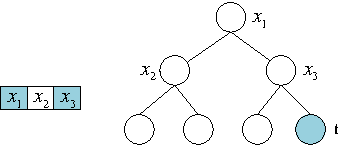
\includegraphics[scale=1.4]{chap04/关键字段}
\end{center}
\caption{关键字段解释}
\label{关键字段}
\end{figure}


细粒度导向模糊测试基本框架主要包括训练和测试两部分,如图\ref{细粒度导向fuzzing基本框架}所示。

训练的目的是产生一个模型,同时计算每个关键字段的权重。给定一个原始的测试用例,此模型能够输出哪些关键字段能够使测试用例与目标区域的距离减小。初始测试用例经过变异生成新的测试用例(此处变异为AFL的原始变异);测试用例通过执行引擎生成执行迹,计算每个执行迹到目标区域的距离,并与原始测试用例做比较;如果距离改变,则将变异后的测试用例$x^{'}$相对于测试用例$x$改变的位置$x \oplus x^{'}$,与距离的改变作为自变量和因变量输入到LSTM网络(Long Short Term)以训练模型,同时累积各个位置距离的变化值以计算权重,并将权重值放入一个全局的权重表中。

测试的目的是基于训练的模型和字段权重引导模糊测试快速执行到目标区域,测试阶段的测试用例是随机挑选的。对于每一个测试用例,使用LSTM模型计算关键字段;根据每个字段的权重,对关键字段进行细粒度变异,生成测试用例;经过执行引擎生成执行迹并测量距离,若距离减小则保留测试用例以待再次变异,反之丢弃;重复测试过程直到满足设定的停机条件。

\begin{figure}[htb]
\begin{center}
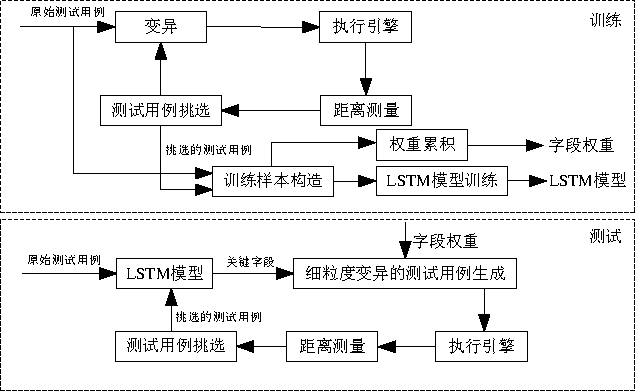
\includegraphics[scale=1.4]{chap04/细粒度导向fuzzing基本框架}
\end{center}
\caption{细粒度导向模糊测试基本框架}
\label{细粒度导向fuzzing基本框架}
\end{figure}

\section{基于LSTM的关键字段获取与权重计算}
\label{基于LSTM的关键字段获取}

本节对应图\ref{细粒度导向fuzzing基本框架}的训练部分,目的是获取对于距离减少起作用的关键字节区域,以及每个bit的权重,主要包括三个部分:衡量测试用例执行迹与目标区域距离的测度、基于LSTM的关键字段获取架构以及字段的权重计算。

\subsection{距离测度}
\label{距离测度}

本节采用AFL-go\upcite{bohme_directed_2017}的距离测度作为产生测试用例的工具。AFL-go是一个用于补丁测试和崩溃重现的工具,在静态分析的基础上能有效的调度AFL逼近目标区域,本章方法采用其距离测度表示测试用例到目标区域的距离。其中,每一个目标区域在源代码中表示为一行代码,在软件的自动测试中,程序执行到某行代码和执行到对应的基本块意义相同,所以到某行代码的距离和到代码所在基本块的距离相同。

\subsubsection{函数距离}

函数距离指的是在函数调用图中两个函数的距离。函数$n$和$n^{'}$的距离记为$d_{f}(n,n^{'})$,表示在函数调用图中两函数之间边的数量。函数$n$到目标函数集$T_f$之间的距离$d_f (n,T_f)$可以定义为$n$到$T_f$中所有函数距离的调和平均数,如式~(\ref{函数到目标函数集的距离})所示。

\begin{equation}\label{函数到目标函数集的距离}
s(X)=\left\{
\begin{aligned}
& undefined, & \text{如果} R(n, T_{f}) = \emptyset \\
& \lbrack \sum_{t_f \in R(n, T_{f})}d_{f}(n,t_{f})^{-1}\rbrack ^{-1} & \text{其他}
\end{aligned}
\right.
\end{equation} 

其中,$R(n,T_{f})$表示在$T_f$中和$n$具有可达关系的函数。调和平均数是总体各统计变量倒数的算术平均数的倒数。主要是用来解决在无法掌握总体单位数(频数)的情况下,只有每组的变量值和相应的标志总量,而需要求得平均数的情况下使用的一种数据方法。调和平均值的计算公式如式~(\ref{调和平均数})所示。相对于算术平均数,在多个目标情况下,调和平均能够区分距离一个目标较近离另外一个目标较远的点与多个目标中间点。如图\ref{调和平均数和算术平均值区别}所示,假设每个线段代表距离1,则中间三个点到$t_1$和$t_2$的算术平均值距离都是2;以调和平均数计算距离,如果一个点有一端比较靠近的某个目标,其距离比中间点的距离要小。本方法的目标是要尽可能的到达目标区域,所以调和平均数较为合适。

\begin{equation}\label{调和平均数}
H_{n} = \frac{n}{\sum_{i=1}^{n}}
\end{equation}

\begin{figure}[htb]
\begin{center}
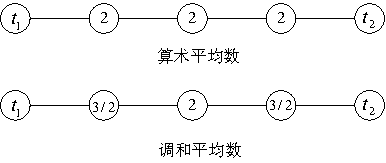
\includegraphics[width=10cm]{chap04/调和平均数和算术平均值区别}
\end{center}
\caption{调和平均数和算术平均值区别}
\label{调和平均数和算术平均值区别}
\end{figure}

\subsubsection{基本块距离}

虽然在程序的全局控制流图计算基本块的距离非常精确,但是全局的控制流图非常复杂,路径搜索和距离求解较为复杂,所以过程间、全局的基本块距离在这里使用过程内的基本块距离和函数距离去近似。如果函数距离越小,则函数之间的基本块的距离也越小。在一个函数$i$的控制流图$G_i$中,设定$d(m_1,m_2)$为$m_1$和$m_2$之间边的数量;$N(m)$为在基本块$m$中调用的函数中,与$T_f$函数具有可达关系的集合,即$N(m) = \{n | R(n, T_f) \neq \emptyset \}$;$T$表示在$G_i$中所有包含函数调用且此函数和$T_f$中函数具有可达关系,即$\forall m \in T.N(m) \neq \emptyset$。基于以上设定,每个基本块$m$与目标基本块集$T_b$的距离定义如式~(\ref{基本块到目标基本集的距离})所示。式中$c=10$是一个常量,用于放大函数之间的距离以近似基本块之间的距离,$d_{b}(m,Tb)$中的$m$表示所有的$G_i$中的任意的基本块,$G_i$函数调用图$CG$中任意函数的控制流图。

\begin{equation}\label{基本块到目标基本集的距离}
d_{b}(m,Tb)=\left\{
\begin{aligned}
& 0, & \text{如果} m \in T_{b} \\
& c \cdot \min\limits_{n \in N(m)}(d_{f}(n,T_{f})), & \text{如果} m \in T \\
& \lbrack \sum_{t \in T}(d_{b}(m,t) + d_{b}(t,T_{b}) ^{-1}\rbrack^{-1} & \text{其他}
\end{aligned}
\right.
\end{equation} 

\subsubsection{测试用例与目标区域之间的距离}

测试用例与目标区域之间的距离可以用程序执行测试用例产生的执行迹与目标基本块集的距离表示,距离越小越可能击中目标基本块。$\varphi(s)={b_1,b_2...b_n}$表示测试用例$s$的执行迹,$b_i$为程序执行的基本块。测试用例与目标区域之间的距离如式~(\ref{测试用例与目标区域之间的距离})所示。

\begin{equation}\label{测试用例与目标区域之间的距离}
d(s,T_b) = \frac{\sum_{m \in \varphi(s)} d_{b}(m,T_b) }{|\varphi(s)|}
\end{equation}

归一化后的测试用例与目标基本块集的距离如式~(\ref{归一化后的测试用例与目标区域之间的距离})所示。

\begin{equation}\label{归一化后的测试用例与目标区域之间的距离}
\hat{d}(s,T_b) = \frac{d_{b}(s,T_b)-minD }{maxD-minD}
\end{equation}
其中
\begin{equation}\label{minD和maxD的定义}
\begin{aligned}
& minD = \min\limits_{s_{i} \in S}\lbrack d(s_{i}, T_b) \rbrack \\
& maxD = \max\limits_{s_{i} \in S}\lbrack d(s_{i}, T_b) \rbrack
\end{aligned}
\end{equation}

归一化后,测试用例与目标区域之间的距离$\hat{d} \in [0,1]$。

\subsection{距离的获取方式}
AFL是一种运行非常速度非常快的模糊测试工具,如果在运行时动态测量测试用例到目标区域之间的距离会大大降低模糊测试的效率,所以本方法在编译时就将基本块之间的距离插桩到代码中以减少AFL动态运行负荷\upcite{bohme_directed_2017}。本方法采用LLVM编译器对源码进行编译和插桩,用于距离测量的的静态插桩如图\ref{用于距离测量的的静态插桩}所示。

\begin{figure}[htb]
\begin{center}
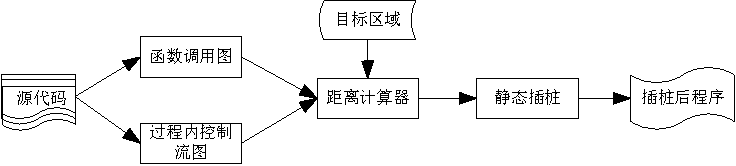
\includegraphics[scale=1.2]{chap04/用于距离测量的的静态插桩}
\end{center}
\caption{用于距离测量的的静态插桩}
\label{用于距离测量的的静态插桩}
\end{figure}

静态插桩的具体过程如下:

(1)产生程序的函数调用图和相应的过程内控制流图。函数调用图用函数声明表示;过程内控制流图用进入函数的第一个语句表示。二者通过编写相应的LLVM Pass\upcite{noauthor_writing_nodate}生成。

(2)基本块之间的距离通过函数之间的距离以及过程内基本块的距离一起计算,详细的计算方式见\ref{距离测度}节。基本块之间距离的计算是通过调用Djikstra算法计算最短距离完成的。

(3)在每个基本块的跳转语句之后插入代码片段用于记录覆盖的控制流边。AFL使用64kb的共享内存存储边在执行过程中的遍历情况,每一条边对应一个字节。在64位的架构中,额外增加了另外16kb内存,8kb用于记录距离值,另外8kb用于记录经过的基本块距离。静态插桩主要实现了两种功能,记录基本块到目标区域的距离以及将遍历的基本块记录到共享内存。

\subsection{训练过程}

\subsubsection{目标函数}

训练的目的是建立一个模型,给定一个测试用例,此模型能够输出一个位图用于表示哪些关键字段的改变能够使测试用例和目标区域的距离减少。因为测试用例是变长的,所以此模型可以被描述为一个函数簇,如式~(\ref{byte目标模型})所示。此函数簇的输入是任意数量的输入位置,输出的是各个位置的变异引起测试用例和目标区域距离减少的概率。

\begin{equation}\label{byte目标模型}
\{f_{k}: \{0x00, 0x01, ...,0xFF \}^{k} \rightarrow [0,1]^{k} | k \in N \}
\end{equation}

式~(\ref{bit目标模型})是以字节为单位判断是否有距离改变,但程序经常会用一个bit进行分支判断,所以需要进一步设定bit级的目标函数,如式~(\ref{bit目标模型})所示。

\begin{equation}\label{bit目标模型}
\{f^{'}_{k}: \{0,1 \}^{8k} \rightarrow [0,1]^{8k} | k \in N \}
\end{equation}

在测试阶段,训练出的模型会首先根据当前测试用例相对于变异前的测试用例所改变的位置,判断是否会引起距离的减少;若减少距离减少则执行此测试用例,反之丢弃,决策函数如式~(\ref{决策函数})所示。式中$x$表示测试用例,$x^{'}$表示变异后的测试用例,$\oplus$表示逐位异或运算,$(x \oplus x^{'})$表示测试用例变异的位置,$\alpha$是一个阈值,控制改变bit的最小数量。式~(\ref{决策函数})的主要思想是判断哪些关键bit上的改变才能够减小到目标区域的距离。

\begin{equation}\label{决策函数}
\sum_{k}(f^{'}(x \oplus x^{'})) > \alpha
\end{equation}

为了训练目标函数$f^{'}$,需要测试用例$x$,变异后的测试用例$x^{'}$,$x$到目标的距离$d(x)$以及$x^{'}$到目标之间的距离$d(x^{'})$;结合这四个参数可以设定一个生成一个有监督的数据集,如式~(\ref{训练集})所示。

\begin{equation}\label{训练集}
xy = \{(x, x \oplus x^{'}) | \bigtriangleup (d(x),d(x^{'})) \neq 0 \}
\end{equation}

\subsubsection{训练模型选择}

因为测试用例的长度是可变的,且bit之间存在关联,本方法使用循环神经网络(Recurrent Neural Network,RNN)训练决策函数。RNN非常适用于处理像程序测试用例这样的序列数据\upcite{rodriguez_recurrent_1999}。因为RNN具有记忆功能,所以RNN在处理有格式的文件输入时非常有用。RNN已经成功的应用于统计机器翻译当中\upcite{cho_learning_2014,bahdanau_neural_2014},本章要处理的问题和此相似,因为测试用例也可以当做是一种语言。

但是RNN很难处理较长的序列,所以本方法采用时间递归神经网络(Long Short-Term Memory,LSTM)\upcite{hochreiter_long_1997}。相对于RNN,LSTM在最顶层增加了一条名为”cell state“的信息传送带同时,所以能够处理更长的序列。同时,LSTM丢弃超过生命周期的序列记忆,以增加处理更长序列的能力。LSTM的一个循环单元(recurrent unit)的状态更新和输出如式~(\ref{循环单元})所示。

\begin{equation}\label{循环单元}
h_{t}, o_{t} = f(x_{t},h_{t-1})
\end{equation}

将式~(\ref{循环单元})分解,如下式~(\ref{LSTM分解})所示。其中,$\sigma$是Sigmoid函数,$W_{*}$为学习的权重向量,$b_{*}$是学习的误差向量。$f_t$是忘记门层,$i_t$是输入门层二者决定是否保留或者丢弃当前输入。通过三种门交织处理使得LSTM能够处理更长的序列。

\begin{equation}\label{LSTM分解}
\begin{aligned}
& f_{t} = \sigma(W_{f} \centerdot [x_{t}, h_{t-1}] + b_f) \\
& i_t = \sigma (W_{i} \centerdot [x_{t}, h_{t-1}] + b_{i}) \\
& C_{t} = f_{t} \times C_{t-1} + i_{t} \times tanh(W_C \centerdot [x_{t}, h_{t-1}] + b_{C}) \\
& o_t = \sigma(W_{o} \centerdot [x_{t}, h_{t-1}] + b_{o}) \\
& h_{t} = o_{t} \times tanh(C_{t})
\end{aligned}
\end{equation}

\subsubsection{关键字段权重计算}
\label{关键字段权重计算}

本方法用一个哈希表存储所有bit的权重,每个bit的权重计算如~(\ref{bit权重计算})所示。其中,$x$和$x^{'}$表示变异前测试用例和变异后的测试用例,$sum(x \oplus x^{'})$表示$x^{'}$相对于$x$变化的字节数量,$\bigtriangleup (d(x),d(x^{'})$表示$x^{'}$相对于$x$减少的距离。式~(\ref{bit权重计算})表示将$\bigtriangleup (d(x),d(x^{'})$平均的分配在改变的每个bit上。训练结束后将权重累积到所有bit位置上,对权重进行归一化,得到bit权重的最终结果。

\begin{equation}\label{bit权重计算}
\omega^{k}_{i}=\left\{
\begin{aligned}
& \omega_{i} =\,| \bigtriangleup (d(x),d(x^{'})) \,|\,/sum(x \oplus x^{'}), & \text{如果 } i \in \{ x \oplus x^{'} \}\\
& 0 & \text{其他}
\end{aligned}
\right.
\end{equation} 

\begin{equation}\label{bit权重累积}
\omega_{i} = \sum_{k=1} \omega^{k}_{i}
\end{equation}

在实际训练的过程中,并不是所有的bit的权重都不相同,本方法将具有相同bit权重的bit集合称之为bit集。

\subsubsection{关键字段权重与程序执行路径的关系}

%\upcite{meng_assisting_2017}发给超哥的自己文章的参考文献格式
本节利用图\ref{权重与程序执行路径的关系实例程序}中的程序描述关键字段权重与程序执行路径之间的关系。图\ref{字段权重和程序执行路径的关系}是图\ref{权重与程序执行路径的关系实例程序}的执行树,每个节点代表一个基本块,第6行的代码和图中红色节点相对应,这里将此基本块表示为$t$;叶子节点下面的字符($a,b,c,d,e,f,g,h$)代表的是执行到相应节点的路径。若要执行$h$,需要的条件是$x1>0 \wedge x3>10 \wedge x7>100$。

假设当前的测试用例$s=(-1,-2,1,-200,1,1,1)$,执行的路径是$a$,按照\ref{距离测度}节的距离计算方式,$d(s,a) = 3$。任意修改$x2,x4,x5$所生成新测试用例$s^{'}$,其与h的距离$d(s,s^{'})$都不会减少。若要减少到h的距离,$x1$必须要大于0,如此在训练的过程中,$x1$的权重则会增加,且$x1$的权重一定大于$x2,x4,x5$。$s$经过变异后生成$s^{'}=(1,-2,1,-200,1,1,1)$,执行的路径是e。对于$s^{'}$,若要减少到h的距离就必须要变异$x3$,从而导致$x3$的权重增加。

在对大量样本进行训练的情况下,关键字段权重能够反应测试用例和输入的关系。对于每一个测试用例,根据其关键字段的权重能够更容易的到达目标区域。

\begin{figure}[h]
\begin{lstlisting}[language=C]
void f(int x1, int x2, int x3, int x4, int x5, int x6, int x7)
{
	if(x1 > 0){
		if(x3 > 10){
			if(x7 > 100)
				target();
		}else{
			if(x6 > 15){
				normal();
			}else
				normal();
		}
			
	}else{
		if(x2 < -1){
			if(x4 < -125){
				normal();
			}else
				normal();
		}else{
			if(x5 < -256){
				normal();
			}else
				normal();
		}
	}
}
\end{lstlisting}
\caption{权重与程序执行路径的关系实例程序}
\label{权重与程序执行路径的关系实例程序}
\end{figure}



\begin{figure}[htb]
\begin{center}
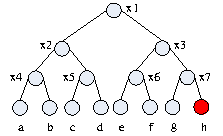
\includegraphics[scale=3]{字段权重和程序执行路径的关系}
\end{center}
\caption{图\ref{权重与程序执行路径的关系实例程序}的执行树}
\label{字段权重和程序执行路径的关系}
\end{figure}


\section{基于细粒度变异的动态测试}
\label{基于字段权重的模糊测试能量调度策略}

本节重点论述在AFL的原有能量调度基础上,基于关键字段和模拟退化算法设计能量调度策略。本章使用的能量的含义是指模糊测试中对一个测试用例的变异次数。

\subsection{细粒度变异的测试用例生成过程}

图\ref{细粒度变异的测试用例生成过程}是本方法采用的通过细粒度变异生成测试用例的过程。对于测试用例$s$,LSTM模型输出使距离减少的bit集,对照全局权重表形成归一化后的bit集,每个bit集的权重用$\omega^{'}_{i}$表示。对于每一个测试用例基于模拟退火框架生成一个能量$p$,按照bit集的权重重新计算每个bit集的权重$p_i$,能量越大表明该bit集变异的次数越多。通过对靠近目标区域的测试用例分配更多的能量,以及对每个bit集根据权值进行细粒度变异能够使测试用例以更大的可能性更快的到距离更近的测试用例,以此增加导向性模糊测试的效率。

\begin{figure}[htb]
\begin{center}
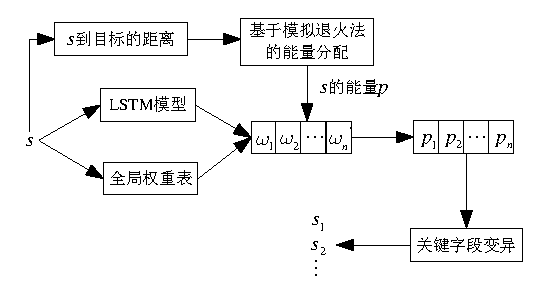
\includegraphics[scale=1.4]{细粒度变异的测试用例生成过程}
\end{center}
\caption{细粒度变异的测试用例生成过程}
\label{细粒度变异的测试用例生成过程}
\end{figure}


\subsection{细粒度变异能量分配策略}

AFL通过测试用例的执行时间、覆盖的基本块数量以及测试用例的深度(测试用例相对与初始测试用例变异的次数)来决定当前测试用例的能量。AFL初始的能量分配策略是以代码覆盖率为导向的,并不适合特定目标导向。本节基于字段权重,在AFL-go\upcite{bohme_directed_2017}的基础上,研究了一种细粒度模拟退火框架的能量分配策略。此策略的主要思想是对距离目标区域较近的测试用例变异能更容易击中目标区域。具体实施时,为距离目标区域较近的测试用例分配更高的能量,从而能以更高的可能性生成到达目标区域的测试用例。

模拟退火法\upcite{kirkpatrick_optimization_1983}的出发点是基于物理学中固体物质的退火过程与一般组合优化问题之间的相似性。模拟退火算法从某一较高初温出发,伴随温度参数的不断下降,结合概率突跳特性在解空间中随机寻找目标函数的全局最优解,即在局部最优解能概率性地跳出并最终趋于全局最优。模拟退火算法是一种通用的优化算法,理论上算法具有概率的全局优化性能。温度是模拟退火的一个重要参数,随着温度的降低,较差解决方案的接受率也降低。在算法开始运行时,初始温度$T=T_0=1$,此时算法接受较差解决方案的概率较高,当$T$接近于0时,算法退化为经典的梯度下降算法。

将模拟退火算法的框架应用到导向模糊测试中想要达到的效果是:测试开始时即温度较高时,允许以较高的概率变异那些距离目标区域较远测试用例,随着时间的推移这种概率越来越低,到时间趋于无穷时只变异距离目标区域最近的测试用例。现在最流行的冷却方案是指数冷却方案\upcite{kirkpatrick_optimization_1983},如式~(\ref{模拟退火算法})所示。其中,$\alpha<1$是个常量,$\alpha$的区间为$[0.8,0.99]$。

\begin{equation}\label{模拟退火算法}
T_{exp} = T_0 \centerdot \alpha^{k}
\end{equation}

在用模糊测试方法挖掘漏洞时,一定会设定一个时间限制$t_x$。在使用模拟退火框架设计能量分配策略时,也需要设定一个$t_x$。在$t_x$之前是导向模糊测试的搜索路径阶段,在此阶段分配给距离较远的测试用例较大的能量,以搜索更多的路径。在$t_x$之后导向模糊测试进入收敛阶段,在此阶段分配给距离最近的测试用例的能量几乎达到最大,使产生的测使用例更好的逼近目标区域。在到达$t_x$时,模拟退火算法等价于梯度下降算法,距离目标区域最近的测试用例分配的最高的能量,让AFL着重变异和测试最有希望击中目标区域的测试用例。假设设置经过$k$轮的迭代之后$T_{exp}=0.1$,则在时间$t$的温度$T_exp$可以通过式~(\ref{t时间温度的计算})的推导获得。同样,可以将$T_{exp}$设置为其他的值,$T_{exp}$越小温度降低的越快。

\begin{equation}\label{t时间温度的计算}
\begin{aligned}
& \alpha^{k_{l}} = 0.1 & \text{当经过}k_{l}\text{轮迭代之后}\\
& k_{l} = log(0.1)/log(a) &\text{求解}k_{l}\\
& T_{exp} = \alpha^{t/t_{x} \centerdot (log(0.1)/log(a))} & \text{将}k_{l}\text{代入}\\
& T_{exp} = 10^{-t/t_{x}} &\text{化简}
\end{aligned}
\end{equation}

模拟退火的温度参数随着时间的增加而减少的,而基于模拟退火框架的能量分配的目的是距离近的测试用例的能量随着时间的增加越来越高,距离大的测试用例的能量随时间的增加越来越低。所以在式~(\ref{t时间温度的计算})的基础上可定义模拟退火的能量分配如式~(\ref{基于模拟退火的能量分配})所示。其中$c_{1}$是一个可调节的常量,控制着搜索阶段距离大的测试用例所分配的能量,$c_{1}$越大距离大的测试用例能量越大。一般地,可以设置$c_{1} = 0.5$;在开始测试时测试距离为1的测试用例的能量为0.5。

\begin{equation}\label{基于模拟退火的能量分配}
\begin{aligned}
& p(m,T_{b}) = (1- \hat{d}(s,T_{b})) \centerdot (1-T_{exp}) + c_{1}T_{exp}
\end{aligned}
\end{equation}

在式~(\ref{基于模拟退火的能量分配})的基础上,可定义每个bit集的变异能量如式~(\ref{关键字段能量})所示,其中,$\omega^{'}_{i}$测试用例关键字段中每个bit的权重。

\begin{equation}\label{关键字段能量}
p_{i} = \frac{\omega^{'}}{\sum_{i} \omega^{'}} \centerdot p(m,T_{b})
\end{equation}

将式~(\ref{关键字段能量})应用到AFL原有的能量策略上,最终的能量分配如式~(\ref{最终能量分配})所示。其中,$c_{2}$是一个常量,用于控制不同距离的能量分配,$c_{2}$越大,距离大的测试用例分配的能量越小,此数值可以在测试时根据不同的目的具体调整。

\begin{equation}\label{最终能量分配}
\hat{p}_{i} = p_{afl}(s) \centerdot 2^{10(p_{i}-c_{2})}
\end{equation}

\section{实验与分析}

\subsection{实验设计}

(1)实验目的

为了测试基于细粒度变异的导向模糊测试方法的有效性,本节在测试效率以及已知漏洞的挖掘数量两个方面进行了实验。

(2)实验环境

%本节主要针对两个目标程序进行实验:readelf\upcite{noauthor_gnu.org_nodate}和libxml2\upcite{noauthor_xml_nodate}。readelf是Linux下binutils中用于分析ELF文件的命令,libxml2是一个XML的C语言解析器和工具库。本实验测试的readelf对应的binutils版本是2.28,libxml2版本是2.9.4,测试软件的基本情况如表\ref{测试软件基本信息}所示。根据CVE数据库的记录libxml2.9.4包含6个漏洞,readelf包含14个漏洞。除了将这些漏洞发生的代码行作为导向的目标区域,还在libxml2的代码中随机标记了42行代码,在readelf代码中随机标记了36行代码作为目标区域。本实验将就目标区域的覆盖数量、目标区域的击中次数以及漏洞的发现数量作为标准衡量本方法的有效性。

本节主要针对readelf\upcite{noauthor_gnu.org_nodate}进行实验。readelf是Linux下binutils中用于分析ELF文件的命令,本实验测试的readelf对应的binutils版本是2.28,测试软件的基本情况如表\ref{测试软件基本信息}所示。根据CVE数据库的记录readelf包含14个漏洞。除了将这些漏洞发生的代码行作为导向的目标区域,还在readelf代码中随机标记了36行代码作为目标区域。本实验将就目标区域的覆盖数量、目标区域的击中次数以及漏洞的发现数量作为标准衡量本方法的可行性和有效性。

\begin{table}[ht]
\begin{center}
\caption{测试软件基本信息}
\label{测试软件基本信息}
\begin{small}
\begin{tabular}{|l|l|l|l|}
\hline
{\bf 软件版本} & {\bf CVE-ID} & {\bf CVE数量} & {\bf 总标记数量} \\
\hline
readelf2.28 & CVE-2017-14333,CVE-2017-15996,CVE-2017-16830 & &\\
& CVE-2017-6965,CVE-2017-6966,CVE-2017-6969 & & \\
& CVE-2017-7209,CVE-2017-8398,CVE-2017-9038 & & \\
& CVE-2017-9039,CVE-2017-9041,CVE-2017-9042 & & \\
& CVE-2017-9043 CVE-2017-9044 & 14 & 50\\
\hline
\end{tabular}
\end{small}
\end{center}
\end{table}

本实验使用Keras\upcite{chollet_keras:_2017}作为前端训练预测模型,选择Tensorflow\upcite{abadi_tensorflow:_2016}作为Keras的底层后端。因为训练测试用例的长度是不同的,而且存在非常大的测试用例一个输入文件可能达到200KB,所以本实验将大于10KB的文件以10KB为单位进行分段。本试验采用Nvidia GTX970 GPUs训练12小时,使用绝对平均误差(Mean Absolute Error,MAE)作为损失函数,使用Adam优化器\upcite{kingma_adam:_2014}以$5 \times 10^{-5}$的学习率训练模型。训练模时可以设定不同的输入输出文件大小,本实验采用的是64bit。

动态导向模糊测试使用的是Inter Xeon CPU E3-1231 v3 @ 3.40GHz,16G RAM,实验设定的搜索路径时间为8小时,8小时后的时间为目标区域导向时间。

(3)实验过程

本实验的实验过程如图\ref{细粒度导向fuzzing基本框架}所示,首先训练与距离相关的关键字段以及关键字段的权重,然后进行动态模糊测试。
本实验的训练所使用的测试用例是由AFL-go产生。刚开始测试时需要搜索更多的路径,所以在运行AFL-go时将式~(\ref{基于模拟退火的能量分配})中的$c_1$设为0.6,给予距离大的测试用例更大的能量,式~(\ref{最终能量分配})中的$c_2$参数设为0.5。本实验运行了AFL-go 6个小时来收集用于训练的样本。将收集的样本按照距离的大小排序,将距离等距的划分为10个区间,即$[0,0.1),[0.1,0.2)...[0.9,1]$。对落入每个区间的测试用例随机的抽取20\%。训练时,每次不放回式抽取两个测试用例,提取每个测试用例与目标区域的距离,按照式~(\ref{训练集})构造样本$xy$。
%
%\begin{equation}\label{构造训练集}
%xy = \{(x,x \oplus x^{'}) | |d(x,x^{'})| > 0\}
%\end{equation}

在动态模糊测试阶段,针对每个测试用例,LSTM模型会输出需要变异的关键字段。关键字段结合全局字段权重表,用于指导字段变异和能量调度,从而近一步指导动态模糊测试的导向性。

\subsection{结果分析}

AFL在判断测试用例是否重复时使用两个标准:(1)程序在执行不同测试用例经过的基本块不相同;(2)经过的基本块相同,但遍历基本块的次数不相同。对于一些有漏洞的危险区域,即使程序执行到目的基本块也不能保证能触发漏洞,例如由循环写造成的缓冲区溢出漏洞,触发此类型的漏洞就需要多次遍历循环内部的基本块。所以可以认为,在测试用例经过的基本块不变的情况下,若能够增加目的区域的遍历次数就更可能触发漏洞。本节将这种能够到达目标区域,经过的基本块相同,但是执行的次数不同的测试用例称为非重复击中目标区域测使用用例。图\ref{非重复击中目标区域测试用例数量对比}是本章方法、AFL-go以及AFL的非重复击中目标区域测使用用例数量的对比。

从图\ref{非重复击中目标区域测试用例数量对比}上可以看出,在8小时之后本章方法和AFL-go非重复击中目标区域测试用例数量增加的速率明显增加,而原始的AFL则没有显著提高。经过24小时本章方法的非重复击中目标区域测试用例数量达到了213个,而AFL-go只达到了127个,AFL只有28个。从非重复击中目标区域测试用例的增加速率以及总数量来看,本章方法要优于AFL-go和AFL。

\begin{figure}[htb]
\begin{center}
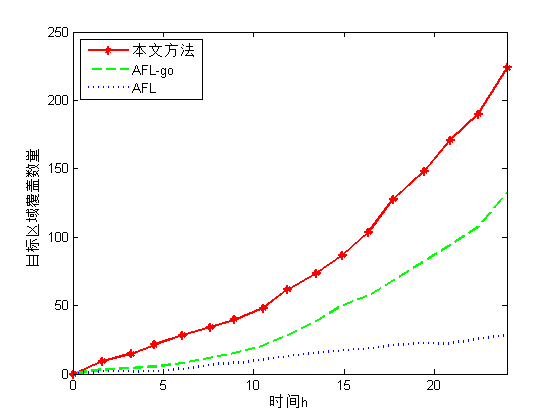
\includegraphics[scale=0.9]{非重复击中目标区域测试用例数量对比}
\end{center}
\caption{非重复击中目标区域测试用例数量对比}
\label{非重复击中目标区域测试用例数量对比}
\end{figure}

图\ref{目标区域覆盖数量对比}是本章方法、AFL-go以及AFL工具在测试readelf时,对标记的50个区域的覆盖情况。从图\ref{目标区域覆盖数量对比}可以看出本章方法和AFL-go在引导模糊测试到达目标区域时具有显著的优势。在8个小时之后,导向目标区域的速率明显增加。本章方法在运行了19小时03分钟之后能够覆盖35个目标区域,AFL-go在执行了20小时35分钟之后覆盖了24个目标区域,而原始的AFL在24个小时之后只能覆盖4个目标区域。实验表明,本章方法在导向目标区域的速率以及覆盖目标区域的数量比AFL-go有明显的提高。

\begin{figure}[htb]
\begin{center}
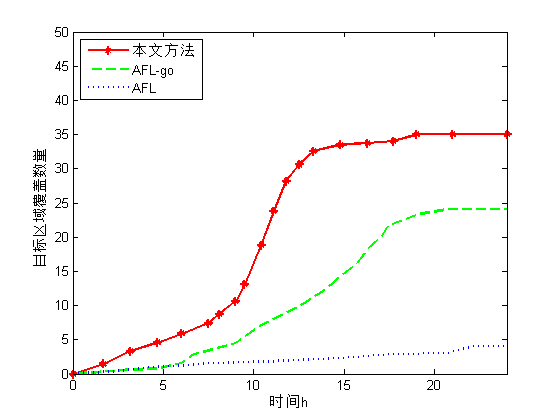
\includegraphics[scale=0.9]{chap04/目标区域覆盖数量对比}
\end{center}
\caption{目标区域覆盖数量对比}
\label{目标区域覆盖数量对比}
\end{figure}

图\ref{发现漏洞数量对比}是本章方法、AFL-go以及AFL工具在测试readelf测试漏洞数量的对比情况。从图\ref{发现漏洞数量对比}可以看出,AFL在24个小时之内没有发现任何漏洞,而在指定目标区域后,本章方法和AFL-go发现的漏洞数量显著增加。本章方法在运行16小时38分钟后发现了9个漏洞,AFL-go在运行了19个小时25分钟后发现了6个漏洞;本章方法在5小时31分钟时发现了第一个漏洞,而AFL-go在8小时13分钟发现了第一个漏洞;说明经过一段时间的路径探索之后本章方法能更早更快的发现漏洞,且最终发现的漏洞比AFL-go多出3个。
\begin{figure}[htb]
\begin{center}
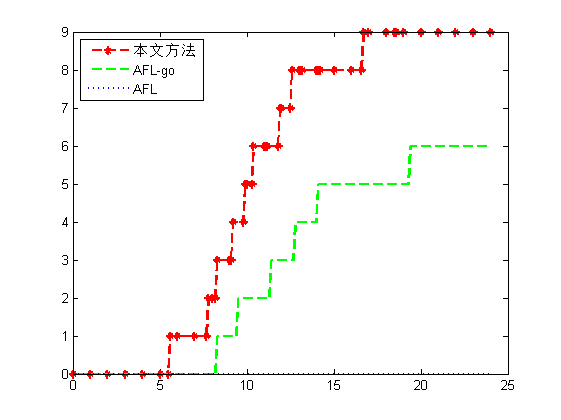
\includegraphics[scale=0.9]{发现漏洞数量对比}
\end{center}
\caption{发现漏洞数量对比}
\label{发现漏洞数量对比}
\end{figure}

\section{本章小节}

本节提出了一种基于细粒度变异的导向模糊测试方法。该方法首先AFL-go收集测试用例;然后利用时间递归神经网络(Long Short-Term Memory,LSTM)训练出一个模型,用于判断哪些字段对靠近目标区域其关键作用,同时收集每个字段的权重;在动态测试测试用例之前,利用上述模型判断对于当前测试用例哪些是关键字段并根据字段权重定向的变异。本章方法能够更细粒度的变异制定的字段,很大程度上消除AFL变异的盲目性,从而能够提高导向模糊测试的效率。

%增加空白页,使下一章的初始页为奇数页
\afterpage{\blankpage}
\chapter{基于细粒度变异的导向模糊测试技术研究}

模糊测试已被证明是一种非常强大的软件漏洞测试方法,是工业界和学术界研究的热点。
%在安全性重要性比较高的软件中,模糊测试发现了绝大多数远程程序执行漏洞和权限提升漏洞。
但是模糊测试一样有它的局限性,盲目的随机的变异测试用例很难到达测试程序的特定路径,导致一些漏洞很难被触发。
在源代码软件的漏洞挖掘中,一些可疑的漏洞触发点可以通过静态分析获取。所以,如何动态的产生测试用例到达可疑漏洞触发点是一项重要的研究内容。现有的主要的导向测试研究都是基于符号执行的\upcite{sparks_automated_2007, santelices_test-suite_2008, person_directed_2011, marinescu_katch:_2013, ma_directed_2011, haller_dowsing_2013, christakis_guiding_2016, bohme_regression_2013},又可称为导向白盒模糊测试。但是导向符号执行在程序分析和约束求解上耗费了大量的时间。在每一轮的测试中,为了到达目标区域,动态符号执行需要利用程序判断哪些分支需要反转,并沿着路径收集约束信息,最后调用约束求解器生成新的输入。而模糊测试不需要约束求解,仅仅通过变异生成测试输入。在相同的时间内,模糊测试产生的输入比动态符号执行高几个数量级。此外,符号执行还有其他的问题如环境交互问题和循环问题\upcite{baldoni_survey_2016}。Macel Bohme\upcite{bohme_directed_2017}提出了一种基于AFL(American fuzzy lop)\upcite{noauthor_american_nodate}的导向模糊测试工具AFL-go。此方法设计了一种用于衡量测试用例到目标区域的距离测度以及一种能量分配策略;随着测试时间的增加,AFL-go通过增加距离近的测试用例的变异次数,减少距离远的测试用例的变异次数,从而完成目标区域导向。但是AFL-go的变异还是具有盲目性,导向效率不高的缺点。
%不能规划测试用例的变异方向的缺点。
%从而导致导向效率不高。

本章提出了一种细粒度变异的导向模糊测试方法。该方法首先AFL-go收集测试用例;然后利用时间递归神经网络(Long Short-Term Memory,LSTM)训练出一个模型,用于判断哪些字段对靠近目标区域其关键作用,同时收集每个字段的权重;在动态运行测试用例之前,利用上述模型判断当前测试用例的关键字段并根据字段权重进行细粒度变异。本文方法能够更细粒度的变异指定字段,很大程度上消除AFL变异的盲目性,从而能够提高导向模糊测试的效率。


\section{反馈式模糊测试技术介绍}\label{模糊测试介绍}

模糊测试是现在最流行的软件测试技术,在很多复杂的程序中发现了很多安全漏洞。模糊测试的主要思想是不间断的产生新的畸形输入让程序执行,以期发现程序的未知行为、崩溃或者异常等行为。通常fuzzer(模糊测试工具)接受一组初始种子输入,通过随机变异或者其他的人为定义的变异策略产生大量的畸形输入反馈给程序执行,直到满足设定的停机条件。但是若遇到输入的格式特别复杂的情况,有时会需要产生数百万次的畸形输入的输入才能触发程序异常。

AFL(American fuzzy lop)\upcite{noauthor_american_nodate}是目前为止最先进的反馈式fuzzer,由Michał Zalewski于2015年开发完成并开源授予大众使用。相对于其他的fuzzer,AFL采用了多种数据变异策略和减少资源耗费的设置,并且不需要复杂的配置,能无缝的处理复杂真实软件,例如图像处理软件和文件压缩库软件。

AFL的优势主要在于其利用遗传算法对测试用例进行优化选择。
AFL维护一个种子测试用例队列,凡是能够提升代码覆盖率的测试用例都将作为种子测试用例,并且增加其新一轮的变异次数;反之,则丢弃。同时,该队列会通过一系列的筛选策略进行优化,以保证优先测试最优测试用例。AFL已经成功的在很多开源软件中发现了很多安全漏洞\upcite{baldoni_survey_2016},例如:Mozilla Firefox,ffmpeg,OpenSSL\upcite{noauthor_american_nodate}等。

AFL进行模糊测试测试的过程如算法\ref{AFL模糊测试}所示。算法输入为待测程序P、初始种子测试用例集以及每个样本的变异次数limit,第4到12行描述的是输入文件变异的详细过程,这里只描述了以字节为单位的变异。除了字节变异,AFL还包含如比特反转、随机替换/插入、已知字典、边界值等变异方式。另外,还采用了组合变异方法,将简单变异随机串联成为复杂变异,从而提高了变异样本覆盖新路径的能力。通过执行变异后的输入文件获取程序的结果result以及路径覆盖信息coverage(第13行);如果result是崩溃信息,则将其加入到MaliciousInputs中(第14-16行);如果路径覆盖coverage增加,则将对应输入input加入到种子序列中(第17-19行)。循环执行上述过程,直到时间耗尽(第21-23行)。

\begin{algorithm}
	\renewcommand{\algorithmicrequire}{\textbf{Input:}}
	\renewcommand{\algorithmicensure}{\textbf{Output:}}
	\caption{AFL模糊测试算法}
	\label{AFL模糊测试}
	\begin{algorithmic}[1]
		\REQUIRE seeds,待测程序 P,每个样本变异次数 limit
		\ENSURE 畸形测试用例 MaliciousInputs
		\STATE c1 = 0
		\FOR{seed in seeds}
			\WHILE{c1 < limit }
				\STATE input = seed
				\STATE length = len(seed)
				\STATE mutations = RandInt(length)
				\STATE mut = 0
				\WHILE{mut < mutations}
					\STATE byte = RandInt(length)
					\STATE mutate(input,byte)
					\STATE mut = mut+1
				\ENDWHILE
				\STATE result,coverage = execute(P,input)
				\IF{result is crash}
					\STATE MaliciousInputs.add(result)
				\ENDIF
				\IF{isIncreased(coverage)}
					\STATE seeds.add(input)
				\ENDIF
			\ENDWHILE
			\IF{timeout()}
				\STATE break
			\ENDIF
		\ENDFOR
	\end{algorithmic}
\end{algorithm}

AFL利用fork server机制增加执行效率。linux程序在执行到main函数之前会经过三个步骤:内核加载程序文件、调用libc\_start\_main以及初始化必要的数据结构和线程环境。一般的fuzzer在每次执行测试用例时都会完整的执行此三个步骤,造成模糊测试速度缓慢。而AFL在程序执行到main函数时,封存此时的状态,当程序再次执行测试用例时,利用linux的fork机制复制一个完全相同的进程,从而省略了上述的三个步骤。以执行binutils程序为例,AFL一秒钟能执行2000次个测试用例而一般的fuzzer只能执行不到100次。



\section{基本框架设计}

本文方法的目的是使用细粒度的变异方法尽快的生成能够到达目标区域的测试用例以挖掘漏洞或者验证程序的安全性。方法的前提条件有两个:(1)指定目标区域,在源代码中以危险操作语句的行数和文件名称表示(例如valid.c:6410);(2)LLVM bitcode插桩,用于编译时计算每个基本块到目标区域的距离,距离的定义见\ref{距离测度}节。

程序执行的路径由输入确定,所以若要控制程序执行到特定区域,相应的输入满足一定条件。图\ref{关键字段}是一个简单的示意图,右半部分是程序的执行路径,左半部分是程序的输入,若想要控制程序执行到关键区域$t$,则需要$x_1$和$x_3$满足一定条件;在本章方法中,$x_1$和$x_3$被称为关键字段。这里的字段是指测试用例中每个比特的位置。

\begin{figure}[htb]
\begin{center}
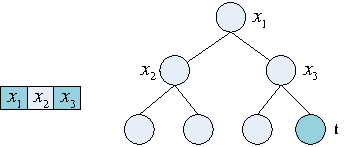
\includegraphics[scale=1.4]{关键字段}
\end{center}
\caption{关键字段解释}
\label{关键字段}
\end{figure}


细粒度导向模糊测试基本框架主要包括训练和测试两部分,如图\ref{细粒度导向fuzzing基本框架}所示。

训练的目的是产生一个模型;给定一个测试用例,此模型能够输出哪些关键字段能够使测试用例与目标区域的距离减小;同时训练计算每个关键字段的权重。初始测试用例经过变异生成新的不同的测试用例,此处变异为AFL的原始变异;测试用例通过执行引擎生成执行迹,计算每个执行迹到目标区域的距离,并与原始测试用例做比较;如果距离减小,则将测试用例改变的位置$x \oplus x^{'}$与相应的改变的距离输入到LSTM网络(Long Short Term)以训练模型;在利用LSTM网络训练的同时累积各个位置距离的变化值以计算权重。

测试的目的是利用训练的模型和字段权重引导模糊测试执行到目标区域。测试阶段的测试用例是训练阶段中与目标区域距离较小的一部分测试用例;利用基于字段权重的能量调度策略(\ref{基于字段权重的模糊测试能量调度策略}节)进行变异生成新的测试用例;经过执行引擎生成执行迹并测量距离,若距离减小则保留测试用例以待再次变异,反之丢弃,重复测试过程直到满足设定的停机条件。

\begin{figure}[htb]
\begin{center}
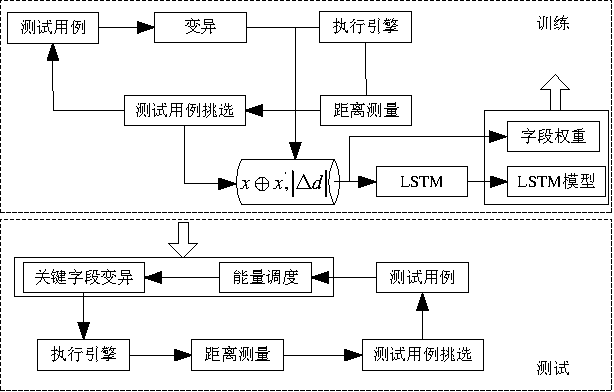
\includegraphics[scale=1.4]{细粒度导向fuzzing基本框架}
\end{center}
\caption{细粒度导向模糊测试基本框架}
\label{细粒度导向fuzzing基本框架}
\end{figure}

\section{基于LSTM的关键字段获取与权重计算}
\label{基于LSTM的关键字段获取}

本节对应图\ref{细粒度导向fuzzing基本框架}的训练部分,目的是获取对于距离减少起作用的关键字节区域,以及每个bit的权重,主要包括三个部分:衡量测试用例执行迹与目标区域距离的测度、基于LSTM的关键字段获取架构以及字段的权重计算。

\subsection{距离测度}
\label{距离测度}

本节采用AFL-go\upcite{bohme_directed_2017}的距离测度作为产生测试用例的工具。AFL-go是一个用于补丁测试和崩溃重现的工具,在静态分析的基础上能有效的调度AFL逼近目标区域,本章方法采用了其距离测度表示测试用例到目标区域的距离。其中,每一个目标区域在源代码中表示为一行代码,在软件的自动测试中,程序执行到某行代码和执行到对应的基本块意义相同,所以到某行代码的距离和到代码所在基本块的距离相同。

\subsubsection{函数距离}

函数距离指的是在函数调用图中两个函数的距离。函数$n$和$n^{'}$的距离记为$d_{f}(n,n^{'})$,表示在函数调用图中两函数之间边的数量。则函数$n$到目标函数集$T_f$之间的距离$d_f (n,T_f)$可以定义为$n$到$T_f$中所有函数距离的调和平均数,如式~(\ref{函数到目标函数集的距离})所示。

\begin{equation}\label{函数到目标函数集的距离}
s(X)=\left\{
\begin{aligned}
& undefined, & \text{如果} R(n, T_{f}) = \emptyset \\
& \lbrack \sum_{t_f \in R(n, T_{f})}d_{f}(n,t_{f})^{-1}\rbrack ^{-1} & \text{其他}
\end{aligned}
\right.
\end{equation} 

其中,$R(n,T_{f})$表示在$T_f$中和$n$具有可达关系的函数。调和平均数是总体各统计变量倒数的算术平均数的倒数。主要是用来解决在无法掌握总体单位数(频数)的情况下,只有每组的变量值和相应的标志总量,而需要求得平均数的情况下使用的一种数据方法。调和平均值的计算公式如式~(\ref{调和平均数})所示。相对于算术平均数,在多个目标情况下,调和平均能够区分距离一个目标较近离另外一个目标较远的点与多个目标中间点。如图\ref{调和平均数和算术平均值区别}所示,假设每个线段代表距离1,则中间三个点到$t_1$和$t_2$的算术平均值距离都是2;以调和平均数计算距离,如果一个点有一端比较靠近的某个目标,其距离比中间点的距离要小。本文方法的目标是要尽可能的到达目标区域,所以调和平均数较为合适。

\begin{equation}\label{调和平均数}
H_{n} = \frac{n}{\sum_{i=1}^{n}}
\end{equation}

\begin{figure}[htb]
\begin{center}
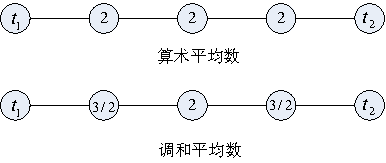
\includegraphics[width=10cm]{调和平均数和算术平均值区别}
\end{center}
\caption{调和平均数和算术平均值区别}
\label{调和平均数和算术平均值区别}
\end{figure}

\subsubsection{基本块距离}

虽然在程序的全局控制流图计算基本块的距离非常精确,但是全局的控制流图非常复杂,路径搜索和距离求解较为复杂,所以过程间、全局的基本块距离在这里使用过程内的基本块距离和函数距离去近似。如果函数距离越小,则函数之间的基本块的距离也越小。在一个函数$i$的控制流图$G_i$中,设定$d(m_1,m_2)$为$m_1$和$m_2$之间边的数量;$N(m)$为在基本块$m$中调用的函数中,与$T_f$函数具有可达关系的集合,即$N(m) = \{n | R(n, T_f) \neq \emptyset \}$;$T$表示在$G_i$中所有包含函数调用且此函数和$T_f$中函数具有可达关系,即$\forall m \in T.N(m) \neq \emptyset$。基于以上设定,每个基本块$m$与目标基本块集$T_b$的距离定义如式 ~(\ref{基本块到目标基本集的距离})所示。式中$c=10$是一个常量,用于放大函数之间的距离以近似基本块之间的距离,$d_{b}(m,Tb)$中的$m$表示所有的$G_i$中的任意的基本块,$G_i$函数调用图$CG$中任意函数的控制流图。

\begin{equation}\label{基本块到目标基本集的距离}
d_{b}(m,Tb)=\left\{
\begin{aligned}
& 0, & \text{如果} m \in T_{b} \\
& c \cdot \min\limits_{n \in N(m)}(d_{f}(n,T_{f})), & \text{如果} m \in T \\
& \lbrack \sum_{t \in T}(d_{b}(m,t) + d_{b}(t,T_{b}) ^{-1}\rbrack^{-1} & \text{其他}
\end{aligned}
\right.
\end{equation} 

\subsubsection{测试用例与目标区域之间的距离}

测试用例与目标区域之间的距离可以用程序执行测试用例产生的执行迹与目标基本块集的距离表示,距离越小越可能击中目标基本块。$\varphi(s)={b_1,b_2...b_n}$表示测试用例$s$的执行迹,$b_i$为程序执行的基本块。测试用例与目标区域之间的距离如式~(\ref{测试用例与目标区域之间的距离})所示。

\begin{equation}\label{测试用例与目标区域之间的距离}
d(s,T_b) = \frac{\sum_{m \in \varphi(s)} d_{b}(m,T_b) }{|\varphi(s)|}
\end{equation}

归一化后的测试用例与目标基本块集的距离如式~(\ref{归一化后的测试用例与目标区域之间的距离})所示。

\begin{equation}\label{归一化后的测试用例与目标区域之间的距离}
\hat{d}(s,T_b) = \frac{d_{b}(s,T_b)-minD }{maxD-minD}
\end{equation}
其中
\begin{equation}\label{minD和maxD的定义}
\begin{aligned}
& minD = \min\limits_{s_{i} \in S}\lbrack d(s_{i}, T_b) \rbrack \\
& maxD = \max\limits_{s_{i} \in S}\lbrack d(s_{i}, T_b) \rbrack
\end{aligned}
\end{equation}

归一化后,测试用例与目标区域之间的距离$\hat{d} \in [0,1]$。

\subsection{距离的获取方式}
AFL是运行非常快速的模糊测试器,如果在运行时动态测量测试用例到目标区域之间的距离会大大降低模糊测试的效率,所以本文采用在编译时将基本块之间的距离插桩到代码的方式来减少AFL动态运行负荷\upcite{bohme_directed_2017}。本文采用LLVM编译器对源码进行编译和插桩,用于距离测量的的静态插桩如图\ref{用于距离测量的的静态插桩}所示。

\begin{figure}[htb]
\begin{center}
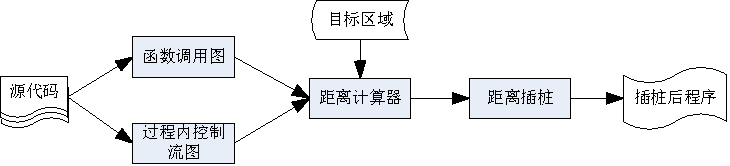
\includegraphics[scale=1.2]{用于距离测量的的静态插桩}
\end{center}
\caption{用于距离测量的的静态插桩}
\label{用于距离测量的的静态插桩}
\end{figure}

静态插桩的具体过程如下:

(1)产生程序的函数调用图和相应的过程内控制流图。函数调用图用函数声明表示;过程内控制流图用进入函数的第一个语句表示。二者通过编写相应的LLVM Pass生成。

(2)基本块之间的距离通过函数之间的距离以及过程内基本块的距离一起计算,详细的计算方式见\ref{距离测度}节。基本块之间距离的计算是通过调用Djikstra算法计算最短距离完成的。

(3)在每个基本块的跳转语句之后插入代码片段用于记录覆盖的控制流边。AFL使用64kb的共享内存存储边在执行过程中的遍历情况,每一条边对应一个字节。在64位的架构中,额外增加了另外16kb内存:8kb用于记录距离值另外8kb用于记录经过的基本块距离。静态插桩主要实现了两种功能:记录基本块到目标区域的距离以及将遍历的基本块记录到共享内存。

\subsection{训练过程}

\subsubsection{目标函数}

训练的目的是建立一个模型,给定一个测试用例,此模型能够输出一个位图用于表示哪些关键字段的改变能够使测试用例和目标区域的距离减少。因为测试用例是变长的,所以此模型可以被描述为一个函数簇,如式~(\ref{byte目标模型})所示。此函数簇的输入是任意数量的输入位置,输出的是各个位置的变异引起测试用例和目标区域距离减少的概率。

\begin{equation}\label{byte目标模型}
\{f_{k}: \{0x00, 0x01, ...,0xFF \}^{k} \rightarrow [0,1]^{k} | k \in N \}
\end{equation}

式~(\ref{bit目标模型})是以字节为单位判断是否有距离改变,但程序经常会用一个bit进行分支判断,所以本文进一步设定了bit级的目标函数,如式~(bit目标模型)所示。

\begin{equation}\label{bit目标模型}
\{f^{'}_{k}: \{0,1 \}^{8k} \rightarrow [0,1]^{8k} | k \in N \}
\end{equation}

在测试阶段,训练出的模型会首先根据当前测试用例相对于变异前的测试用例所改变的位置,去判断是否会引起距离的减少;若减少距离减少则执行此测试用例,反之丢弃,决策函数如式~(\ref{决策函数})所示。式中$x$表示测试用例,$x^{'}$表示变异后的测试用例,$\oplus$表示逐位异或运算,$(x \oplus x^{'})$表示测试用例变异的位置,$\alpha$是一个阈值,控制改变bit的最小数量。式~(\ref{决策函数})的主要思想是判断哪些关键bit上的改变才能够减小到目标区域的距离。

\begin{equation}\label{决策函数}
\sum_{k}(f^{'}(x \oplus x^{'})) > \alpha
\end{equation}

为了训练目标函数$f^{'}$,需要测试用例$x$,变异后的测试用例$x^{'}$,$x$到目标的距离$d(x)$以及$x^{'}$到目标之间的距离$d(x^{'})$;结合这四个参数可以设定一个生成一个有监督的数据集,如式~(\ref{训练集})所示。

\begin{equation}\label{训练集}
xy = \{(x, x \oplus x^{'}) | \bigtriangleup (d(x),d(x^{'})) > 0 \}
\end{equation}

\subsubsection{训练模型选择}

因为测试用例的长度是可变的,且bit之间存在关联,本文使用循环神经网络(Recurrent Neural Network,RNN)训练决策函数。RNN非常适用于处理像程序测试用例这样的序列数据\upcite{rodriguez_recurrent_1999}。因为RNN的记忆功能,所以RNN在处理有格式的文件输入时非常有用。RNN已经成功的应用于统计机器翻译当中\upcite{cho_learning_2014,bahdanau_neural_2014},本章要处理的问题和此相似,因为测试用例也可以当做是一种语言。

但是RNN很难处理较长的序列,所以本文采用时间递归神经网络(Long Short-Term Memory,LSTM)。相对于RNN,LSTM在最顶层增加了一条名为”cell state“的信息传送带同时,所以能够处理更长的序列。同时,LSTM丢弃超过生命周期的序列记忆,以增加处理更长序列的能力。LSTM的一个循环单元(recurrent unit)的状态更新和输出如式~(\ref{循环单元})所示。

\begin{equation}\label{循环单元}
h_{t}, o_{t} = f(x_{t},h_{t-1})
\end{equation}

将式~(\ref{循环单元})分解,如下式~(\ref{LSTM分解})所示。其中,$\sigma$是Sigmoid函数,$W_{*}$为学习的权重向量,$b_{*}$是学习的误差向量。$f_t$是忘记门层,$i_t$是输入门层二者决定是否保留或者丢弃当前输入。通过三种门交织处理使得LSTM能够处理更长的序列。

\begin{equation}\label{LSTM分解}
\begin{aligned}
& f_{t} = \sigma(W_{f} \centerdot [x_{t}, h_{t-1}] + b_f) \\
& i_t = \sigma (W_{i} \centerdot [x_{t}, h_{t-1}] + b_{i}) \\
& C_{t} = f_{t} \times C_{t-1} + i_{t} \times tanh(W_C \centerdot [x_{t}, h_{t-1}] + b_{C}) \\
& o_t = \sigma(W_{o} \centerdot [x_{t}, h_{t-1}] + b_{o}) \\
& h_{t} = o_{t} \times tanh(C_{t})
\end{aligned}
\end{equation}

\subsubsection{关键字段权重计算}
\label{关键字段权重计算}

本文用一个哈希表存储所有bit改变引起的距离的改变,每个bit的权重计算如~(\ref{bit权重计算})所示。其中,$x$和$x^{'}$表示变异前测试用例和变异后的测试用例,$sum(x \oplus x^{'})$表示$x^{'}$相对于$x$变化的字节数量,$\bigtriangleup (d(x),d(x^{'})$表示$x^{'}$相对于$x$减少的距离。式~(\ref{bit权重计算})表示将$\bigtriangleup (d(x),d(x^{'})$平均的分配在改变的每个bit上。训练结束后将权重累积到所有bit位置上,对权重进行归一化,得到bit权重的最终结果。

\begin{equation}\label{bit权重计算}
\omega^{k}_{i}=\left\{
\begin{aligned}
& \omega_{i} = \bigtriangleup (d(x),d(x^{'}))/sum(x \oplus x^{'}), & \text{如果 } i \in \{ x \oplus x^{'} \}\\
& 0 & \text{其他}
\end{aligned}
\right.
\end{equation} 

\begin{equation}\label{bit权重累积}
\omega_{i} = \sum_{k=1} \omega^{k}_{i}
\end{equation}

在实际训练的过程中,并不是所有的bit的权重都不相同,本文将具有相同bit权重的bit集合称之为bit集。

\subsubsection{关键字段权重与程序执行路径的关系}

本节利用程序Listing \ref{权重与程序执行路径的关系实例程序}论述关键字段权重与程序执行路径之间的关系。图\ref{字段权重和程序执行路径的关系}是Listing \ref{权重与程序执行路径的关系实例程序}的执行树,每个节点代表一个基本块,第6行的代码和图中红色节点相对应,这里将此基本块表示为$t$;叶子节点下面的字符($a,b,c,d,e,f,g,h$)代表的是执行到相应节点的路径。若要执行$h$,需要的条件是$x1>0 \wedge x3>100 \wedge x7>100$。

假设当前的测试用例$s=(-1,-2,1,-200,1,1,1)$,执行的路径是$a$,按照\ref{距离测度}节的距离计算方式,$d(s,a) = 3$。任意修改$x2,x4,x5$所生成新测试用例$s^{'}$,其与h的距离$d(s,s^{'})$都不会减少。若要减少到h的距离,$x1$必须要大于0,如此$x1$的权重则会增加,$x1$的权重一定大于$x2,x4,x5$。$s$经过变异后生成$s^{'}=(1,-2,1,-200,1,1,1)$,执行的路径是e。对于$s^{'}$,若要减少到h的距离就必须要变异$x3$,从而导致$x3$的权重增加。

在对大量样本进行训练的情况下,关键字段权重能够反应测试用例和输入的关系,即权重大的字段能够控制执行树的节点。对于每一个测试用例,根据其关键字段的权重能够更容易的到达目标区域。

\begin{lstlisting}[language=C,caption=权重与程序执行路径的关系实例程序,label=权重与程序执行路径的关系实例程序]
void f(int x1, int x2, int x3, int x4, int x5, int x6, int x7)
{
	if(x1 > 0){
		if(x3 > 10){
			if(x7 > 100)
				target();
		}else{
			if(x6 > 15){
				normal();
			}else
				normal();
		}
			
	}else{
		if(x2 < -1){
			if(x4 < -125){
				normal();
			}else
				normal();
		}else{
			if(x5 < -256){
				normal();
			}else
				normal();
		}
	}
}
\end{lstlisting}

\begin{figure}[htb]
\begin{center}
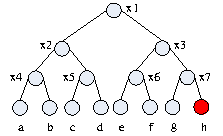
\includegraphics[scale=3]{字段权重和程序执行路径的关系}
\end{center}
\caption{Listing \ref{权重与程序执行路径的关系实例程序}的执行树}
\label{字段权重和程序执行路径的关系}
\end{figure}


\section{动态测试}
\label{基于字段权重的模糊测试能量调度策略}

本节重点论述在AFL的原有能量调度基础上,基于关键字段和模拟退化算法设计能量调度策略。本章使用的能量的含义是指模糊测试中对一个测试用例的变异次数。

\subsection{细粒度变异的测试用例生成过程}

图\ref{细粒度变异的测试用例生成过程}是本文采用的通过细粒度变异生成测试用例的过程。对于测试用例$s$,LSTM模型输出使距离减少的bit集,对照全局权重表形成归一化后的bit集,每个bit集的权重用$\omega^{'}_{i}$表示。对于每一个测试用例基于模拟退火框架生成一个能量$p$,按照bit集的权重重新计算每个bit集的权重$p_i$,能量越大表明该bit集变异的次数越多。通过对靠近目标区域的测试用例分配更多的能量,以及对每个bit集根据权值进行细粒度变异能够使测试用例以更大的可能性更快的到距离更近的测试用例,以此增加导向性模糊测试的效率。

\begin{figure}[htb]
\begin{center}
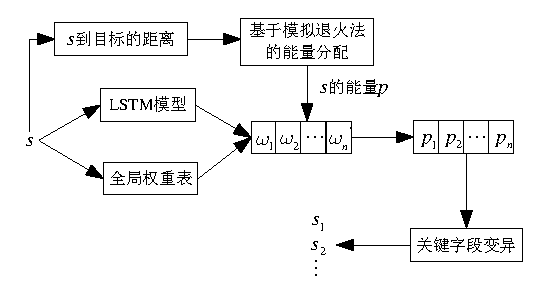
\includegraphics[scale=1.4]{细粒度变异的测试用例生成过程}
\end{center}
\caption{细粒度变异的测试用例生成过程}
\label{细粒度变异的测试用例生成过程}
\end{figure}


\subsection{细粒度变异能量分配策略}

AFL通过测试用例的执行时间、覆盖的基本块数量以及测试用例的深度(测试用例相对与初始测试用例变异的次数)来决定当前测试用例的能量。AFL初始的能量分配策略是以代码覆盖率为导向的,并不适合特定目标导向。本节基于字段权重,介绍一种模拟退火框架的能量分配策略。此策略的主要思想是对距离目标区域较近的测试用例变异能更容易击中目标区域。具体实施时,为距离目标区域较近的测试用例分配更高的能量,从而能以更高的可能性生成到达目标区域的测试用例。

模拟退火法\upcite{kirkpatrick_optimization_1983}的出发点是基于物理中固体物质的退火过程与一般组合优化问题之间的相似性。模拟退火算法从某一较高初温出发,伴随温度参数的不断下降,结合概率突跳特性在解空间中随机寻找目标函数的全局最优解,即在局部最优解能概率性地跳出并最终趋于全局最优。模拟退火算法是一种通用的优化算法,理论上算法具有概率的全局优化性能。温度是模拟退火的一个重要参数,随着温度的降低,较差解决方案的接受率也降低。在算法开始运行时,初始温度$T=T_0=1$,此时算法接受较差解决方案的概率较高,当$T$接近于0时,算法退化为经典的梯度下降算法。

将模拟退火算法的框架应用到导向模糊测试中想要达到的效果是:测试开始时即温度较高时,允许以较高的概率变异那些距离目标区域较远测试用例,随着时间的推移这种概率越来越低,到时间趋于无穷时只变异距离目标区域最近的测试用例。现在最流行的冷却方案是指数冷却方案\upcite{kirkpatrick_optimization_1983},如式~(\ref{模拟退火算法})所示。其中,$\alpha<1$是个常量,$\alpha$的区间为$[0.8,0.99]$。

\begin{equation}\label{模拟退火算法}
T_{exp} = T_0 \centerdot \alpha^{k}
\end{equation}

在用模糊测试方法挖掘漏洞时,一定会设定一个时间限制$t_x$。在使用模拟退火框架设计能量分配策略时,也需要设定一个$t_x$。在$t_x$之前是导向模糊测试的搜索路径阶段,在此阶段分配给距离较远的测试用例较大的能量,以搜索更多的路径。在$t_x$之后导向模糊测试进入收敛阶段,在此阶段分配给距离最近的测试用例的能量几乎达到最大,使产生的测使用例更好的逼近目标区域。在到达$t_x$时,模拟退火算法等价于梯度下降算法,距离目标区域最近的测试用例分配的最高的能量,让AFL着重变异和测试最有希望击中目标区域的测试用例。假设设置经过$k$轮的迭代之后$T_{exp}=0.1$,则在时间$t$的温度$T_exp$可以通过式~(\ref{t时间温度的计算})的推导获得。同样,可以将$T_{exp}$设置为其他的值,$T_{exp}$越小温度降低的越快。

\begin{equation}\label{t时间温度的计算}
\begin{aligned}
& \alpha^{k_{l}} = 0.1 & \text{当经过}k_{l}\text{轮迭代之后}\\
& k_{l} = log(0.1)/log(a) &\text{求解}k_{l}\\
& T_{exp} = \alpha^{t/t_{x} \centerdot (log(0.1)/log(a))} & \text{将}k_{l}\text{代入}\\
& T_{exp} = 10^{-t/t_{x}} &\text{化简}
\end{aligned}
\end{equation}

模拟退火的温度参数随着时间的增加而减少的,而基于模拟退火框架的能量分配的目的是距离近的测试用例的能量随着时间的增加越来越高,距离大的测试用例的能量随时间的增加越来越低。所以在式~(\ref{t时间温度的计算})的基础上可定义模拟退火的能量分配如式~(\ref{基于模拟退火的能量分配})所示。其中$c_{1}$是一个可调节的常量,控制着搜索阶段距离大的测试用例所分配的能量,$c_{1}$越大距离大的测试用例能量越大。典型的,可以设置$c_{1} = 0.5$;在开始测试时测试距离为1的测试用例的能量为0.5。

\begin{equation}\label{基于模拟退火的能量分配}
\begin{aligned}
& p(m,T_{b}) = (1- \hat{d}(s,T_{b})) \centerdot (1-T_{exp}) + c_{1}T_{exp}
\end{aligned}
\end{equation}

在式~(\ref{基于模拟退火的能量分配})的基础上,可定义每个bit集的变异能量如式~(\ref{关键字段能量})所示,其中,$\omega^{'}_{i}$测试用例关键字段中每个bit的权重。

\begin{equation}\label{关键字段能量}
p_{i} = \frac{\omega^{'}}{\sum_{i} \omega^{'}} \centerdot p(m,T_{b})
\end{equation}

将式~(\ref{关键字段能量})应用到AFL原有的能量策略上,最终的能量分配如式~(\ref{最终能量分配})所示。其中,$c_{2}$是一个常量,用于控制不同距离的能量分配,$c_{2}$越大,距离大的测试用例分配的能量越小,此数值可以在测试时根据不同的目的具体调整。

\begin{equation}\label{最终能量分配}
\hat{p}_{i} = p_{afl}(s) \centerdot 2^{10(p_{i}-c_{2})}
\end{equation}

\section{实验结果与分析}

\subsection{实验设计}

(1)实验目的

为了测试基于细粒度变异的导向模糊测试方法的有效性,本节在测试效率以及已知漏洞的挖掘数量两个方面上进行了实验。

(2)实验环境

%本节主要针对两个目标程序进行实验:readelf\upcite{noauthor_gnu.org_nodate}和libxml2\upcite{noauthor_xml_nodate}。readelf是Linux下binutils中用于分析ELF文件的命令,libxml2是一个XML的C语言解析器和工具库。本实验测试的readelf对应的binutils版本是2.28,libxml2版本是2.9.4,测试软件的基本情况如表\ref{测试软件基本信息}所示。根据CVE数据库的记录libxml2.9.4包含6个漏洞,readelf包含14个漏洞。除了将这些漏洞发生的代码行作为导向的目标区域,还在libxml2的代码中随机标记了42行代码,在readelf代码中随机标记了36行代码作为目标区域。本实验将就目标区域的覆盖数量、目标区域的击中次数以及漏洞的发现数量作为标准衡量本文方法的有效性。

本节主要针对readelf\upcite{noauthor_gnu.org_nodate}进行实验。readelf是Linux下binutils中用于分析ELF文件的命令,本实验测试的readelf对应的binutils版本是2.28,测试软件的基本情况如表\ref{测试软件基本信息}所示。根据CVE数据库的记录readelf包含14个漏洞。除了将这些漏洞发生的代码行作为导向的目标区域,还在readelf代码中随机标记了36行代码作为目标区域。本实验将就目标区域的覆盖数量、目标区域的击中次数以及漏洞的发现数量作为标准衡量本文方法的可行性和有效性。

\begin{table}[ht]
\begin{center}
\caption{测试软件基本信息}
\label{测试软件基本信息}
\begin{small}
\begin{tabular}{|l|l|l|l|}
\hline
{\bf 软件版本} & {\bf CVE-ID} & {\bf CVE数量} & {\bf 总标记数量} \\
\hline
readelf2.28 & CVE-2017-14333,CVE-2017-15996,CVE-2017-16830 & &\\
& CVE-2017-6965,CVE-2017-6966,CVE-2017-6969 & & \\
& CVE-2017-7209,CVE-2017-8398,CVE-2017-9038 & & \\
& CVE-2017-9039,CVE-2017-9041,CVE-2017-9042 & & \\
& CVE-2017-9043 CVE-2017-9044 & 14 & 50\\
\hline
\end{tabular}
\end{small}
\end{center}
\end{table}

本实验使用Keras\upcite{chollet_keras:_2017}作为前端训练预测模型,选择Tensorflow\upcite{abadi_tensorflow:_2016}作为Keras的底层后端。因为训练测试用例的长度是不同的,而且存在非常大的测试用例一个输入文件可能达到200KB,所以本实验将大于10KB的文件以10KB为单位进行分段。本试验采用Nvidia GTX970 GPUs训练12小时,使用绝对平均误差(Mean Absolute Error,MAE)作为损失函数,使用Adam优化器\upcite{kingma_adam:_2014}以$5 \times 10^{-5}$的学习率训练模型。训练模时可以设定不同的输入输出文件大小,本实验采用的是64bit。

动态导向模糊测试使用的是Inter Xeon CPU E3-1231 v3 @ 3.40GHz,16G RAM,实验设定的搜索路径时间为8小时,8小时后的时间为目标区域导向时间。

(3)实验过程

本实验的实验过程如图\ref{细粒度导向fuzzing基本框架}所示,首先训练与距离相关的关键字段以及关键字段的权重,然后进行动态模糊测试。
本实验的训练所使用的测试用例是由AFL-go产生。刚开始测试时需要搜索更多的路径,所以在运行AFL-go时将式~(\ref{基于模拟退火的能量分配})中的$c_1$设为0.6,给予距离大的测试用例更大的能量,式~(\ref{最终能量分配})中的$c_2$参数设为0.5。本实验运行了AFL-go 6个小时来收集用于训练的样本。将收集的样本按照距离的大小排序,将距离等距的划分为10个区间,即$[0,0.1),[0.1,0.2)...[0.9,1]$。对落入每个区间的测试用例随机的抽取20\%。训练时,每次不放回式抽取两个测试用例,提取每个测试用例与目标区域的距离,按照式~(\ref{构造训练集})构造样本$xy$。

\begin{equation}\label{构造训练集}
xy = \{(x,x \oplus x^{'}) | |d(x,x^{'})| > 0\}
\end{equation}

在动态模糊测试阶段,针对每个测试用例,LSTM模型会输出需要变异的关键字段。关键字段结合全局字段权重表,用于指导字段变异和能量调度,从而近一步指导动态模糊测试的导向性。

\subsection{结果分析}

AFL在判断测试用例是否重复时使用两个标准:(1)程序在执行不同测试用例经过的基本块不相同;(2)经过的基本块相同,但遍历基本块的次数不相同。对于一些有漏洞的危险区域,即使程序执行到目的基本块也不能保证能触发漏洞,例如由循环写造成的缓冲区溢出漏洞,触发此类型的漏洞就需要多次遍历循环内部的基本块。所以可以认为,在测试用例经过的基本块不变的情况下,若能够增加目的区域的遍历次数就更可能触发漏洞。本节将这种能够到达目标区域,经过的基本块相同,但是执行的次数不同的测试用例称为非重复击中目标区域测使用用例。图\ref{非重复击中目标区域测试用例数量对比}是本章方法、AFL-go以及AFL的非重复击中目标区域测使用用例数量的对比。

从图\ref{非重复击中目标区域测试用例数量对比}上可以看出,在8小时之后本章方法和AFL-go非重复击中目标区域测试用例数量增加的速率明显增加,而原始的AFL则没有显著提高。经过24小时本章方法的非重复击中目标区域测试用例数量达到了213个,而AFL-go只达到了127个,AFL只有28个。从非重复击中目标区域测试用例的增加速率以及总数量来看,本章方法要优于AFL-go和AFL。

\begin{figure}[htb]
\begin{center}
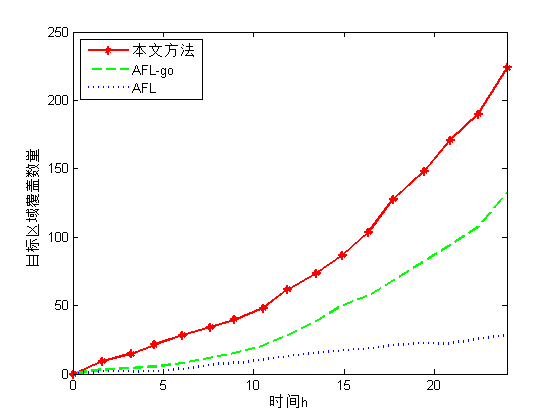
\includegraphics[scale=0.9]{非重复击中目标区域测试用例数量对比}
\end{center}
\caption{非重复击中目标区域测试用例数量对比}
\label{非重复击中目标区域测试用例数量对比}
\end{figure}

图\ref{目标区域覆盖数量对比}是本章方法、AFL-go以及AFL工具在测试readelf时,对标记的50个区域的覆盖情况。从图\ref{目标区域覆盖数量对比}可以看出本章方法和AFL-go在引导模糊测试到达目标区域时具有显著的优势。在8个小时之后,导向目标区域的速率明显增加。本章方法在运行了17小时36分钟之后能够覆盖35个目标区域,AFL-go在执行了22小时21分钟之后覆盖了24个目标区域,而原始的AFL在24个小时之后只能覆盖4个目标区域。实验表明,本章方法在导向目标区域的速率以及覆盖目标区域的数量比AFL-go有明显的提高。

\begin{figure}[htb]
\begin{center}
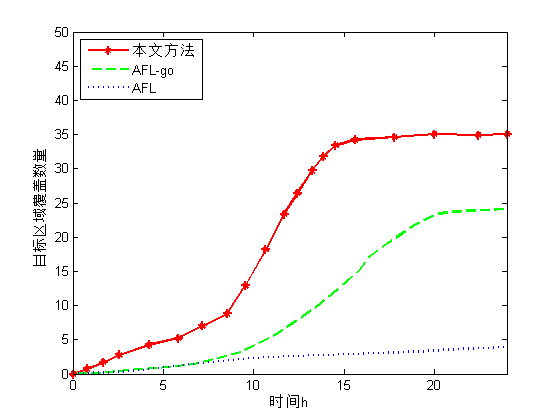
\includegraphics[scale=0.9]{目标区域覆盖数量对比}
\end{center}
\caption{目标区域覆盖数量对比}
\label{目标区域覆盖数量对比}
\end{figure}

图\ref{发现漏洞数量对比}是本章方法、AFL-go以及AFL工具在测试readelf测试漏洞数量的对比情况。从图\ref{发现漏洞数量对比}可以看出,AFL在24个小时之内没有发现任何漏洞,而在指定目标区域后,本章方法和AFL-go发现的漏洞数量显著增加。本章方法在运行16小时38分钟后发现了11个漏洞,AFL-go在运行了19个小时25分钟后发现了6个漏洞;本章方法在5小时31分钟时发现了第一个漏洞,而AFL-go在8小时13分钟发现了第一个漏洞;说明经过一段时间的路径探索之后本章方法能更早更快的发现漏洞,且最终发现的漏洞比AFL-go多出3个。
\begin{figure}[htb]
\begin{center}
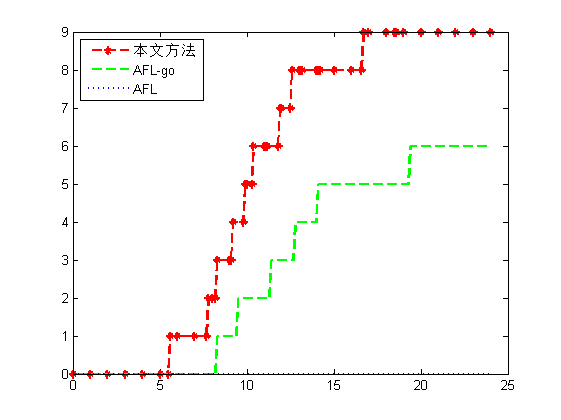
\includegraphics[scale=0.9]{发现漏洞数量对比}
\end{center}
\caption{发现漏洞数量对比}
\label{发现漏洞数量对比}
\end{figure}

\section{本章小节}

本节提出了一种基于细粒度变异的导向模糊测试方法。该方法首先AFL-go收集测试用例;然后利用时间递归神经网络(Long Short-Term Memory,LSTM)训练出一个模型,用于判断哪些字段对靠近目标区域其关键作用,同时收集每个字段的权重;在动态测试测试用例之前,利用上述模型判断对于当前测试用例哪些是关键字段并根据字段权重定向的变异。本章方法能够更细粒度的变异制定的字段,很大程度上消除AFL变异的盲目性,从而能够提高导向模糊测试的效率。
\chapter{总结与展望}

\section{论文主要工作总结}
%syf
%论文以源代码程序漏洞为挖掘目标,分析了当前源代码软件漏洞挖掘面临的主要问
%题,采用先静态分析定位疑似漏洞,后动态
%测试验证疑似漏洞的漏洞挖掘思路,通过把程序静态分析与测试技术相结合,取长补
%短,提高漏洞挖掘的效率。一方面由于静态分析代码覆盖率高,能够获取代码的
%全局信息,因而能够描述的漏洞类型多,漏洞挖掘的漏报率低,另一方面,可以
%通过动态测试的方法验证静态分析发现的漏洞是否为真实漏洞,去除误报。
%同时,采用先静态定位后动态验证的方法使得动态测试的针对性更强,减少了对整个程序盲目测试所带来的时间和资源开销。
%syf

论文通过对比现有软件源代码漏洞挖掘方法及工具,分析源代码软件漏洞挖掘的发展趋势,总结了源代码软件漏洞挖掘存在四个关键问题:(1)多种类源代码软件漏洞精确静态挖掘问题;(2)机器学习算法和源代码软件漏洞挖掘的结合问题;(3)源代码静态信息辅助的模糊测试导向问题;(4)结合形式化方法缓解符号执行的路径爆炸问题。针对以上四个问题,论文研究了多种源代码动、静态分析技术,其主要工作和创新如下:

(1)提出了一种基于程序性质图的源代码软件漏洞挖掘方法。
%用于解决多种源代码漏洞不能通过单一的中间表示检测的问题。
首先,利用语法解析器解析源代码,依次生成语法分析树、抽象语法树、控制流图、数据流图;然后,聚合抽象语法树、控制流图以及数据流图形成程序性质图,并且定义程序性质图的基本遍历方法;最后,根据漏洞的形成模式,组合程序性质图遍历方法检测缓冲区溢出漏洞、格式化字符串漏洞以及Use After Free漏洞。该方法能有效的检测此三类源代码漏洞,并具备扩展的检测其他类型源代码漏洞的能力。

(2)提出了一种基于机器学习的缓冲区溢出漏洞挖掘方法。该方法首先总结了7类缓冲区溢出漏洞静态特征,分别为sink类型、缓冲区位置、容器、索引/地址/长度复杂度、边界检测、循环/条件/函数调用深度以及是否输入可控;其次,通过扩展的程序性质图检测缓冲区溢出漏洞的各类性质并将其向量化;然后,利用有监督机器学习算法在已标记的训练集上训练分类器;最后,利用此分类器在新的源代码程序中挖掘缓冲区溢出漏洞。通过在测试集的对比实验表明,该方法比BOMiner多检测了14.8个的缓冲区溢出漏洞;通过在Linux的驱动程序上的对比实验表明,该方法平均比Joern多发现了8.2个缓冲区溢出漏洞。


(3)提出了一种细粒度变异的导向模糊测试方法。该方法首先利用导向模糊测试收集测试用例;然后利用时间递归神经网络训练出一个模型,用于判断对靠近目标区域起关键作用的字段,同时收集每个字段的权重;最后,通过上述模型判断当前测试用例的关键字段,并利用关键字段权重进行细粒度的变异生成测试用例。通过和导向模糊测试工具AFL-go在测试程序上的对比实验,在24个小时内,该方法比AFL-go多击中87次目标区域;多覆盖11个非重复目标区域;多检测3个漏洞。


(4)提出了一种结合静态程序分析的高效符号执行技术,用于缓解循环程序导致的符号执行路径指数级爆炸问题。该技术首先通过静态程序分析方法,从程序的控制流图中计算出循环程序的不变式;然后,对程序进行插桩用循环不变式代替循环,形成新的控制流图;最后在新的控制流图上进行符号执行。通过100个基准程序上进行的对比实验,本方法FastSE在发现错误的实例数量上,比对循环进行定长展开的KLEE-Fix提高了11.8\%,比原始的KLEE符号执行工具提高了32.6\%;在时间消耗上,分别减少了11.9\%和43.8\%。


\section{下一步工作展望}
%wb
%由于学术水平所限,论文的研究成果还有许多进一步拓展的空间。另一方面,理论的发展技
%术的进步不会停止,这也会引导研究者去寻找新的更好的漏洞挖掘方法。因此,
%未来一段时期内需要进一步研究的主要内容包括:
%wb

(1)论文第三章中研究了基于有监督学习的缓冲区溢出漏洞挖掘方法,
其静态特征需要人为指定,训练数据需要人为标定。特征的指定需要人的经验,训练数据的
标定也是一件非常耗时的工作。所以探索利用深度学习的方法去自动学习漏洞特征是下一步研究方向。

(2)论文第四章研究了基于细粒度变异的导向模糊测试技术,但是其训练和动态测试是分离的两部分,动态测试的
结果不能及时的反馈给训练过程做实时修正,如何将训练过程与动态测试过程联动起来增加测试的效率和效果
是下一步的研究方向。

(3)论文第五章中研究了结合静态程序分析的高效符号执行技术,运用抽象解释的方法求解循环程序的不变式。
虽然能大大增加符号执行的效率,但同时降低了符号执行的精度,会导致产生虚假的测试用例。如何深层次
的结合抽象解释和符号执行技术,在精度和效率之间达到一个更好的平衡是下一步研究的方向。此外,在
已知目标区域的情况下如何进行导向符号执行是另外一个需要研究的工作。



%%% Local Variables:
%%% mode: latex
%%% TeX-master: "../main"
%%% End:

\begin{ack}
  行文至此,心中万分感慨。回顾博士阶段的五年学习生活,经历过认可时的激动和喜悦,也经历过失意时的苦涩和迷茫,少了一份功利,多了一份专注,这些带给我的不仅是科学思维上的磨练,更是全面素质的提升。在此,谨向多年来一直给予我知道、支持帮助的老师、同学和亲人们表示最衷心的感谢,是你们的陪伴和无私帮助激励我不断前行!
  
  衷心感谢我的导师沈荣骏院士。沈院士虽然不在长沙亲身知道,但定期他总要从北京赶来听取学生在课题方面的进展汇报,并给出很多建设性的意见和建议,来长沙出差之际,总是挤出时间和学生交流沟通。
  
  衷心感谢我的博士导师唐朝京教授!我从 2013 年受教于唐老师就读博士研究
  生至今,他严肃认真的治学态度、深厚的学术功底、严密的思维、渊博的知识和
  分析问题、提炼问题的能力,使我在学业上受益匪浅。我在博士论文选题、研究
  和论文写作的整个过程,都是在唐老师的悉心指导和严格要求下完成的。在几年
  的学习过程中,不仅使我的学术水平得到了很大的提高,在学术道德方面,我也
  有了更加深刻的认识,对自己的要求也更为严格。唐老师极富责任感、对待科研
  非常严谨,这种品质深深地影响着我,促使我形成严谨求实的学术作风,这将成
  为我人生的一大笔财富。唐老师还对我的论文写作方面进行了细心的指导,无私
  地传授给我论文写作的大量规律和经验。唐老师对工作认真勤恳的态度以及在学
  术上不断进取的精神永远是我今后工作学习的榜样!在此谨向他表示最衷心的感
  谢和最诚挚的敬意!
  
  衷心感谢张权副教授!是您带领我走进了信息安全研究的科研殿堂。感谢王
  剑教授、刘俭老师、张琛老师、张磊副教授、冯超老师、李瑞林老师等诸位老师对我的指导
  和关心。我在教研室学习期间,他们为我创造了良好的工作环境,他们在学术上
  的执着追求以及一丝不苟的工作作风也使我受
  
  感谢李孟君师兄、吴波师兄、解纬师兄、张博师兄、王少磊师兄、帅博师兄,王强师兄,感谢毕兴、刘毅、张斌、陈夏阳、叶嘉曦、张兴、冯冈夫、黄安琪、在同一个实验室中工作使得我们有了更多的讨论,在相互的交流和学习中我受益良多。
  
  深深的感谢我的家人,没有你们的支持,就没有今天的我!
  
  谨以此文献给所有关心我支持我的亲人和朋友们!

\end{ack}


\cleardoublepage
\phantomsection
\addcontentsline{toc}{chapter}{参考文献}
\bibliographystyle{bstutf8}
\bibliography{ref/refs}
%\bibliography{ref/wb}


\begin{resume}

  \section*{发表的学术论文} % 发表的和录用的合在一起
%公开版
  \begin{enumerate}[{[}1{]}]
%  \addtolength{\itemsep}{-.36\baselineskip}%缩小条目之间的间距,下面类似
  \item Qingkun M, Chao F, Bin Z, Chaojing T. Assisting in Auditing of Buffer Overflow Vulnerabilities via Machine Learning.(SCI检索,检索号:00041904420001)
  
  \item Qingkun M, Shameng W, Bin Z, Chaojing T. Automatically Discover Program Vulnerability Through Similar Functions. PIERS2016.(EI检索,检索号20165203169818)
  
  \item Qingkun M, Bin Z, Chao F, Chaojing T. Detecting Buffer Boundary Violations based on SVM. ICISCE2016. (EI检索,检索号:20165003106907)
  
  \item Qingkun M, Shameng W, Chao F, Chaojing T. Predicting buffer overflow using semi-supervised learning. CISP-BMEI2016.(EI检索,检索号:20171303496365)
  
  \item Qingkun M, Shameng W, Chao F, Chaojing T. Predicting Integer Overflow through Static Integer Operation Attributes. ICCSNT2016. (EI检索,检索号:20180104610722)
  
  \item Shameng W, Qingkun M, Chao F, Chaojing T. Protocol Vulnerability Detection Based on Network Traffic Analysis and Binary Reverse Engineering. PLOS ONE, 2017. (SCI检索 000413195900048)
    
  \item Shameng W, Qingkun M, Chao F, Chaojing T. A Model-Guided Symbolic Execu-
  tion Approach for Network Protocol Implementations and Vulnerability Detection.
  PLOS ONE, 2017. (SCI检索,检索号:000413195900048)
  
  \item Shameng W, Chao F, Qingkun M, Bin Z, Ligeng W, Chaojing T. Testing Network
  Protocol Binary Software with Selective Symbolic Execution. CIS2016. (EI检索,检索号:20171203453840)
  
  \item Shameng W, Chao F, Qingkun M, Bin Z, Ligeng W, Chaojing T. Analyzing Net-
  work Protocol Binary Software with Joint Symbolic Execution. ICSAI2016. (EI检索,检索号:20171203462505)
  
  \item Shameng W, Chao F, Qingkun M, Bin Z, Ligeng W, Chaojing T. Model-Guided
  Symbolic Execution Testing for Network Protocol Binary Software. PIC2016. (EI
  检索,检索号:20173003971908)
  
  \item Shameng W, Chao F, Qingkun M, Bin Z, Ligeng W, Chaojing T. Multi-Packet
  Symbolic Execution Testing for Network Protocol Binary Software. ICCSNT2016.
  (EI检索,检索号:20180104611161)
  
%  \item 
  
  \end{enumerate}
  %盲评版
%  \begin{enumerate}[{[}1{]}]
%  %  \addtolength{\itemsep}{-.36\baselineskip}%缩小条目之间的间距,下面类似
%    \item 第一作者. Assisting in Auditing of Buffer Overflow Vulnerabilities via Machine Learning.(SCI检索,检索号:00041904420001)
%    
%    \item 第一作者. Automatically Discover Program Vulnerability Through Similar Functions. PIERS2016.(EI检索,检索号20165203169818)
%    
%    \item 第一作者. Detecting Buffer Boundary Violations based on SVM. ICISCE2016. (EI检索,检索号:20165003106907)
%    
%    \item 第一作者. Predicting buffer overflow using semi-supervised learning. CISP-BMEI2016.(EI检索,检索号:20171303496365)
%    
%    \item 第一作者. Predicting Integer Overflow through Static Integer Operation Attributes. ICCSNT2016. (EI检索,检索号:20180104610722)
%    
%    \item 第二作者. Protocol Vulnerability Detection Based on Network Traffic Analysis and Binary Reverse Engineering. PLOS ONE, 2017. (SCI检索 000413195900048)
%      
%    \item 第二作者. A Model-Guided Symbolic Execu-
%    tion Approach for Network Protocol Implementations and Vulnerability Detection.
%    PLOS ONE, 2017. (SCI检索,检索号:000413195900048)
%    
%    \item 第三作者. Testing Network
%    Protocol Binary Software with Selective Symbolic Execution. CIS2016. (EI检索,检索号:20171203453840)
%    
%    \item 第三作者. Analyzing Net-
%    work Protocol Binary Software with Joint Symbolic Execution. ICSAI2016. (EI检索,检索号:20171203462505)
%    
%    \item 第三作者. Model-Guided
%    Symbolic Execution Testing for Network Protocol Binary Software. PIC2016. (EI
%    检索,检索号:20173003971908)
%    
%    \item 第三作者. Multi-Packet
%    Symbolic Execution Testing for Network Protocol Binary Software. ICCSNT2016.
%    (EI检索,检索号:20180104611161)
%    
%  %  \item 
%    
%    \end{enumerate}

  \section*{参与的主要科研项目} % 有就写,没有就删除
  \begin{enumerate}[{[}1{]}]
  \addtolength{\itemsep}{-.36\baselineskip}%
  \item XXXX信息系统,海军项目,项目主要负责人.
  \item 全军XXXX装备业务系统,总参项目,项目主要负责人.
  \item XXXX挖掘验证测试技术,国家863项目,项目主要参与者.
  \item 大规模XXXX,2016国家重点研发计划,项目主要参与者.
  \end{enumerate}
\end{resume}

%\input{data/resume_mangping}
% 最后,需要的话还要生成附录,全文随之结束。
% \appendix
\backmatter
% \input{data/appendix_Ma}

\end{document}